\clearpage
\section{Data availability statement}

The original data presented in this chapter are openly available from the \texttt{GitHub} repository:
\href{https://github.com/Photonico/H-Beryllene_20250718}{\texttt{Photonico/H-Beryllene\_20250718}}.

\section{Supplementary information}
\label{3_supplementary}

Convergence tests for the cohesive energy and total energy are shown in figures~\ref{fig:proj3_cohesive_energy_convergence}
and~\ref{fig:proj3_total_energy_convergence},
respectively,
as functions of the k-point set for the beryllium structures.
Convergence tests for the calculation of the dielectric function are shown in figures~\ref{fig:proj3_hcp_dielectric_nbands_convergence}--\ref{fig:proj3_cubic_dielectric_kpoint_convergence},
including tests for both the k-point set and the total number of bands included through the parameter \texttt{NBANDS}.

\begin{figure}[!htbp]
\centering
\begin{tabular}{@{}cc@{}}
    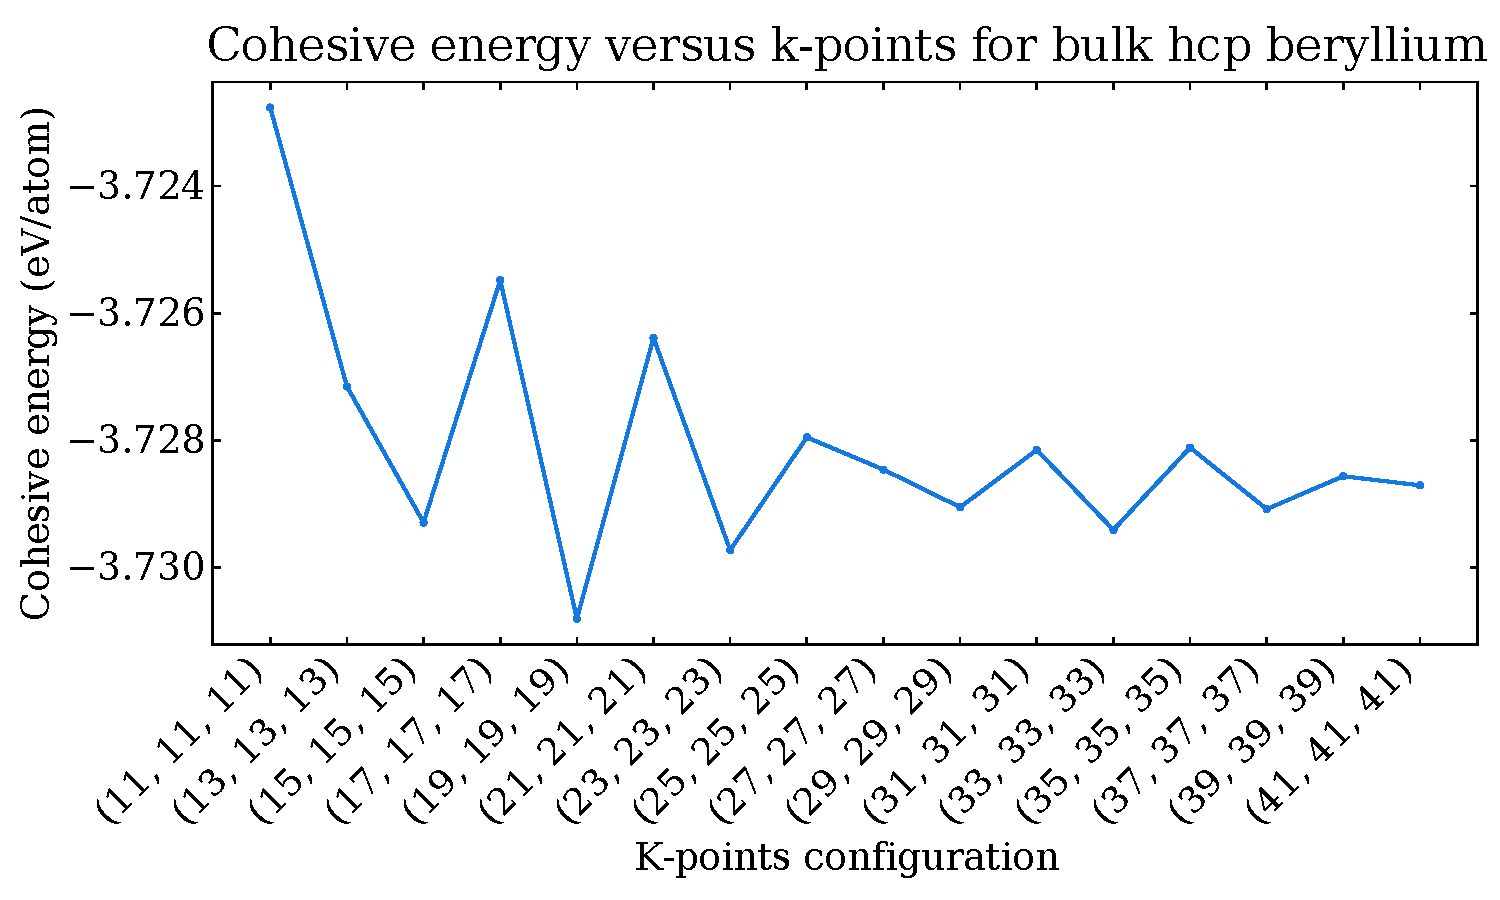
\includegraphics[width=0.40\linewidth]{figures_proj3/convergence_cohesive_kpoints_hcp-beryllium_thesis.pdf}&
    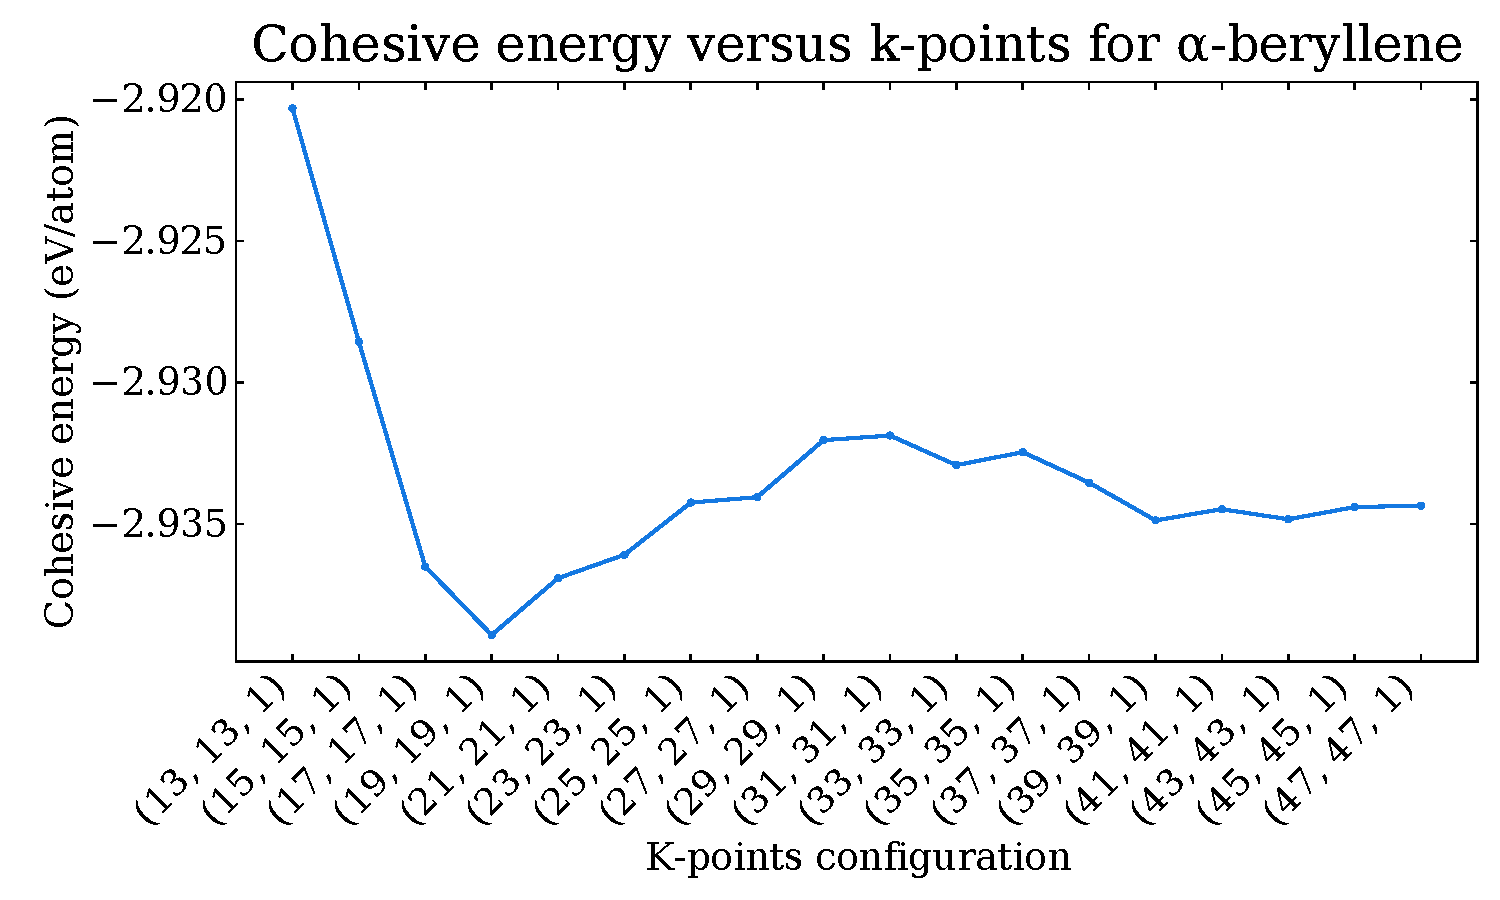
\includegraphics[width=0.40\linewidth]{figures_proj3/convergence_cohesive_kpoints_alpha-beryllene_thesis.pdf}\\
    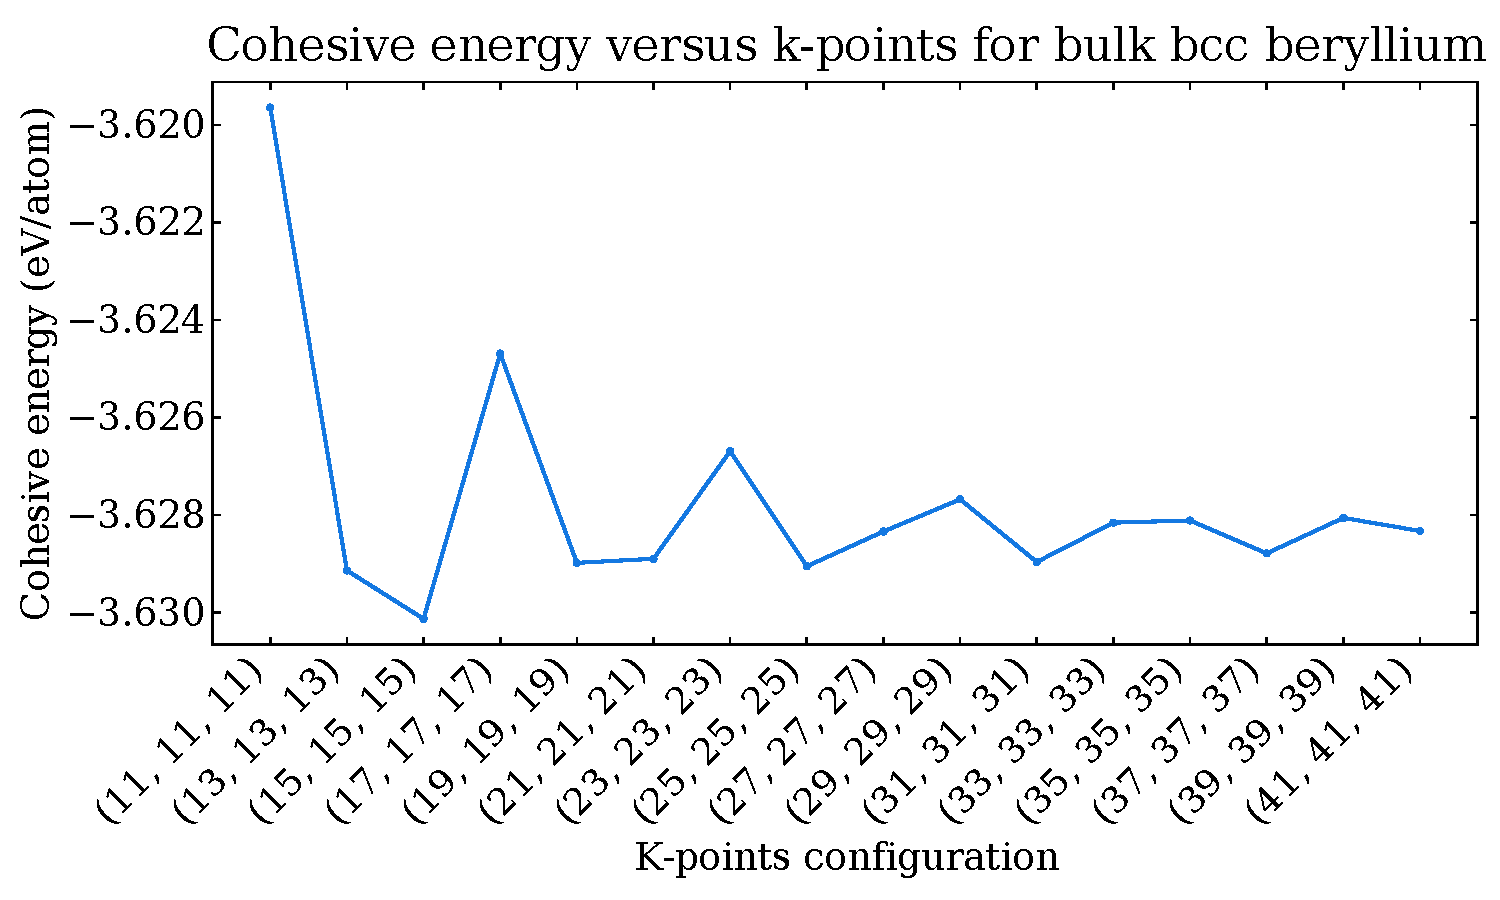
\includegraphics[width=0.40\linewidth]{figures_proj3/convergence_cohesive_kpoints_bcc-beryllium_thesis.pdf}&
    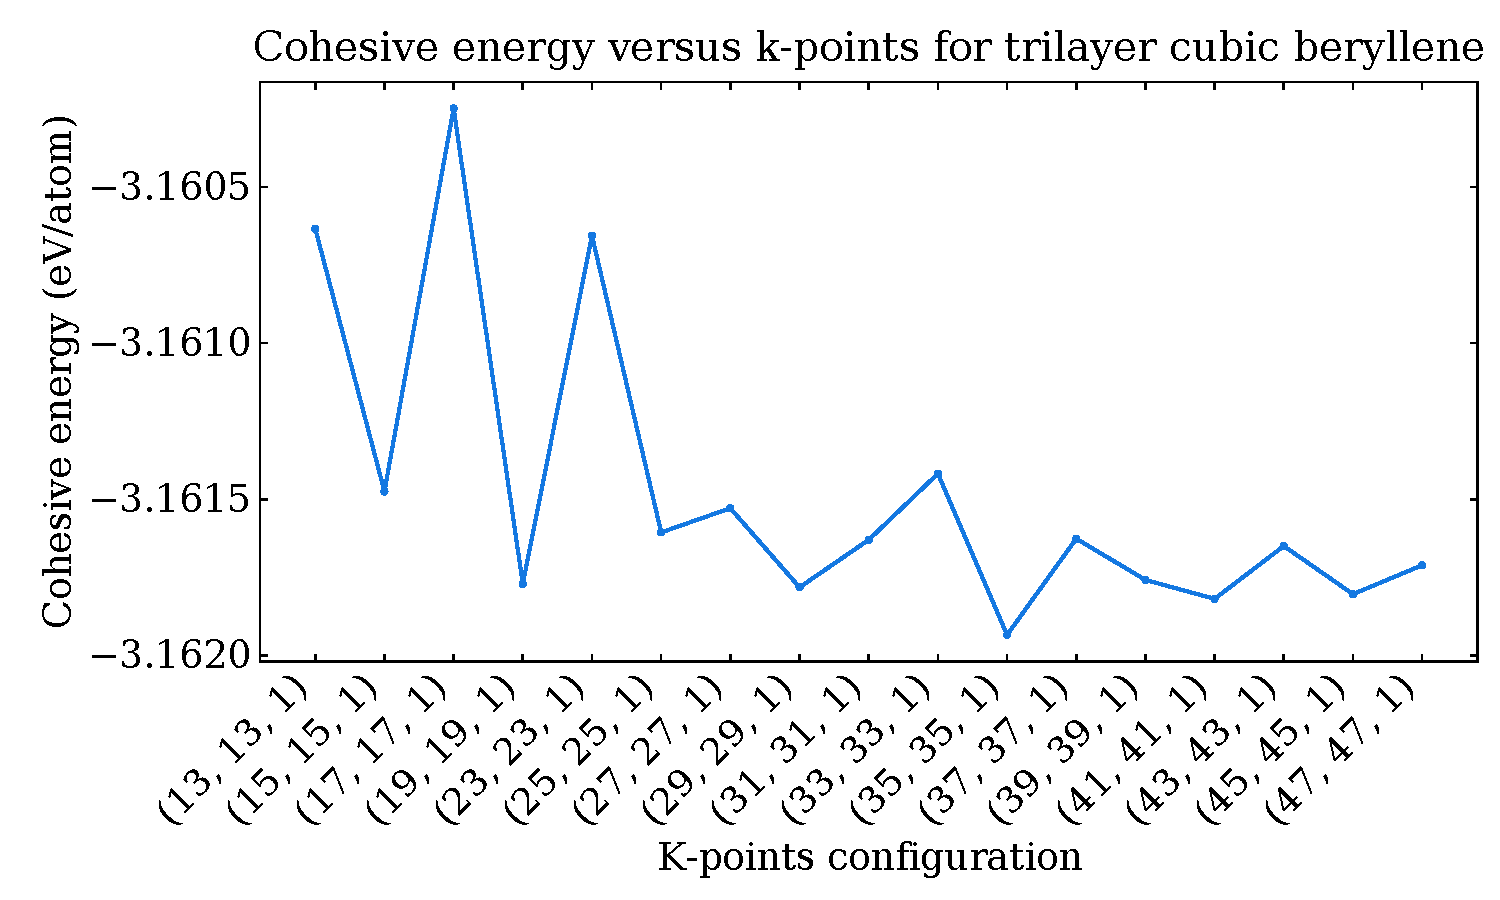
\includegraphics[width=0.40\linewidth]{figures_proj3/convergence_cohesive_kpoints_cubic-beryllene-trilayer_thesis.pdf}
\end{tabular}
\caption{Cohesive energy as a function of k-point set for bulk hcp beryllium, $\alpha$-beryllene, bulk bcc beryllium, and trilayer cubic beryllene.}
\label{fig:proj3_cohesive_energy_convergence}
\end{figure}

\begin{figure}[!htbp]
\centering
\begin{tabular}{@{}cc@{}}
    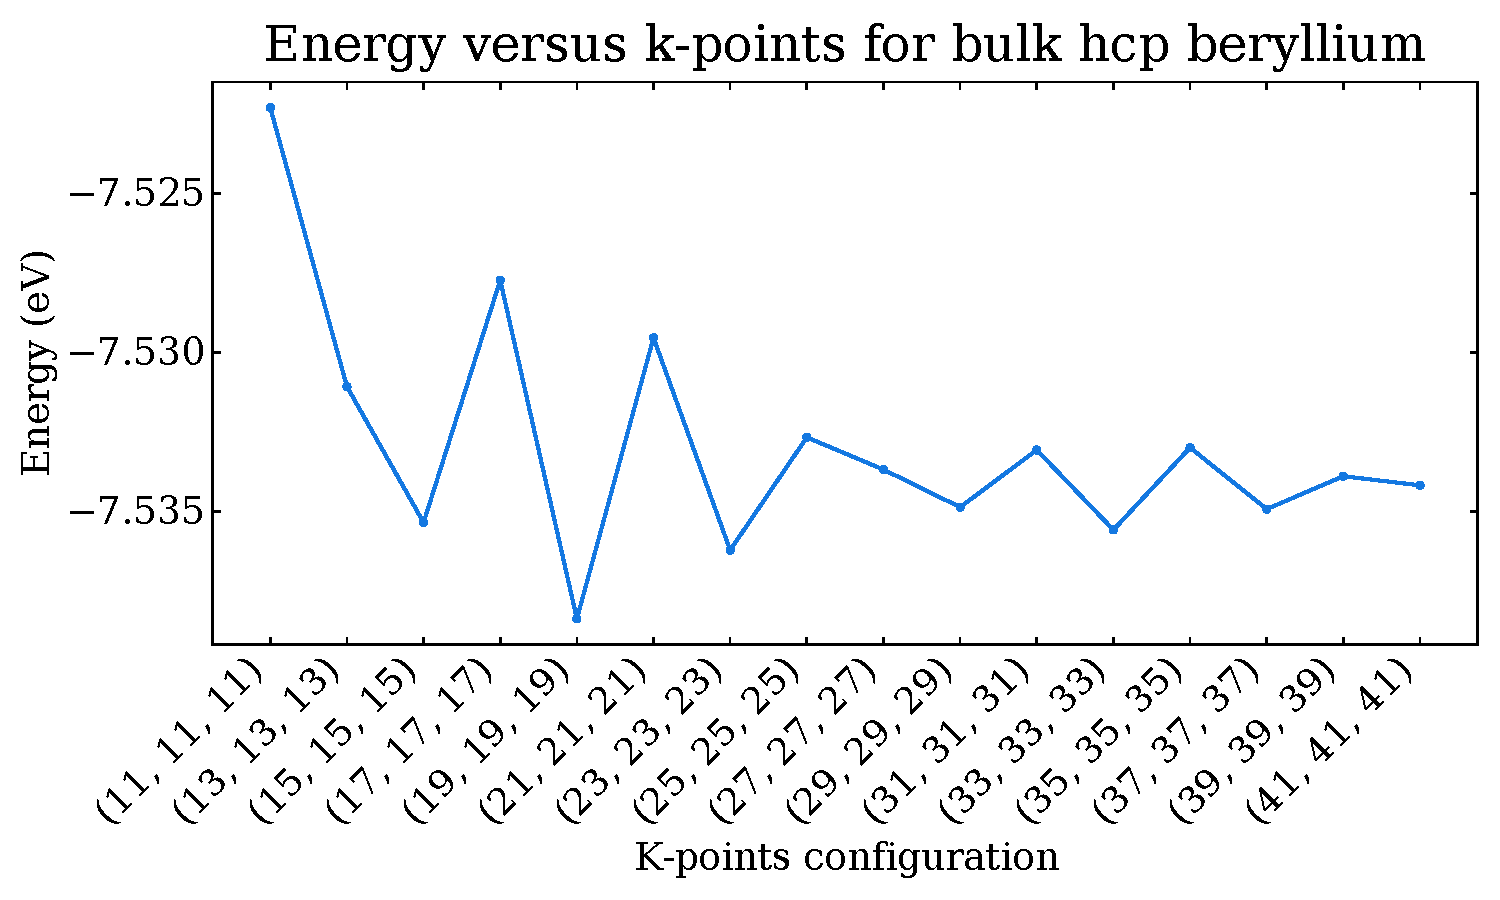
\includegraphics[width=0.40\linewidth]{figures_proj3/convergence_energy_kpoints_hcp-beryllium_thesis.pdf}&
    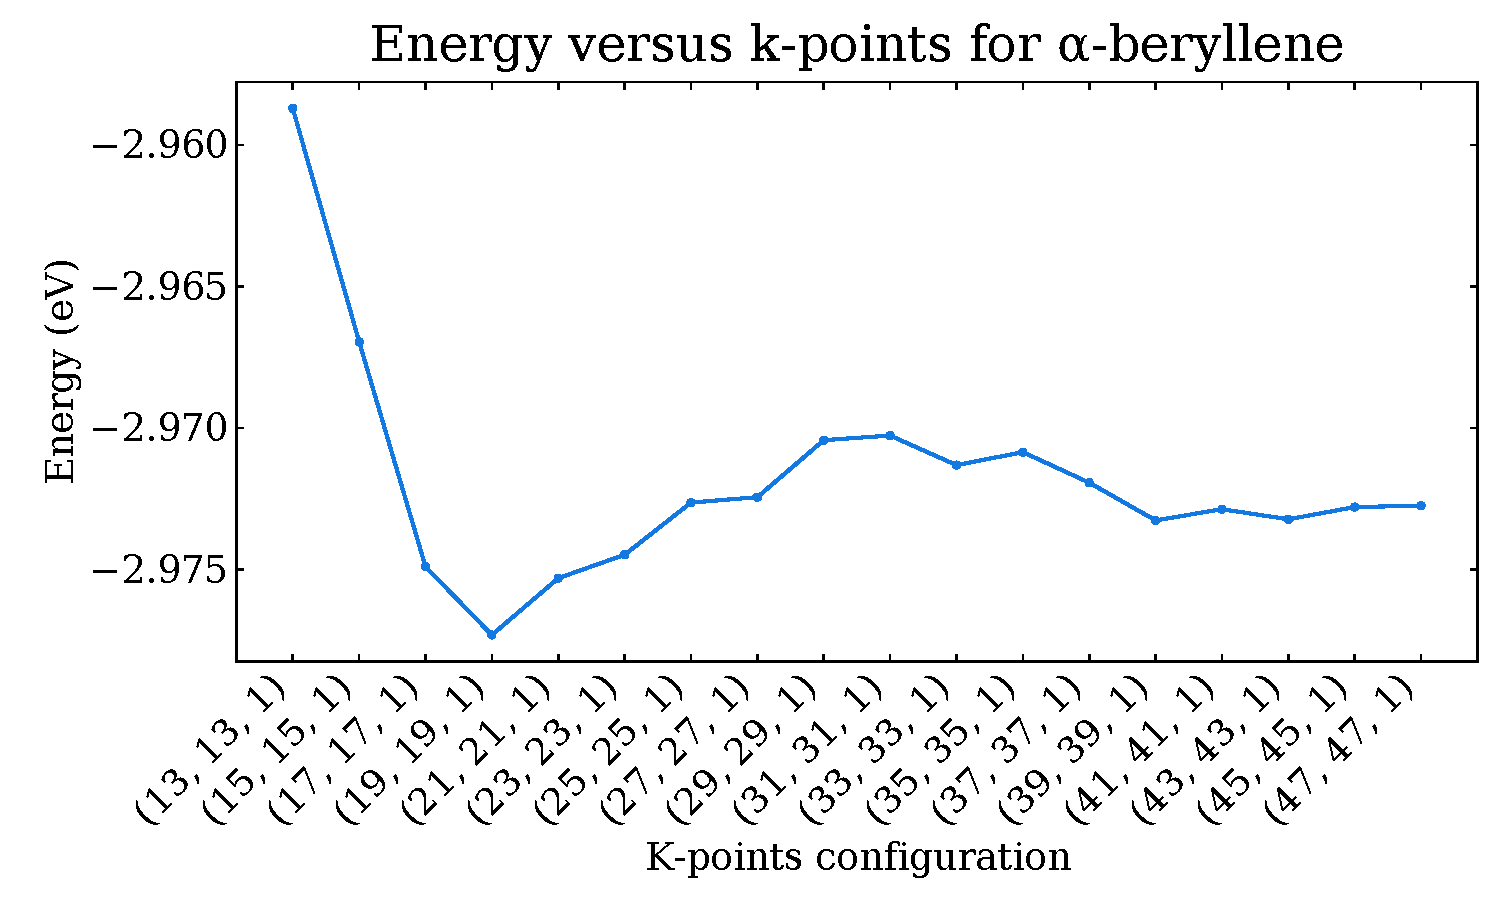
\includegraphics[width=0.40\linewidth]{figures_proj3/convergence_energy_kpoints_alpha-beryllene_thesis.pdf}\\
    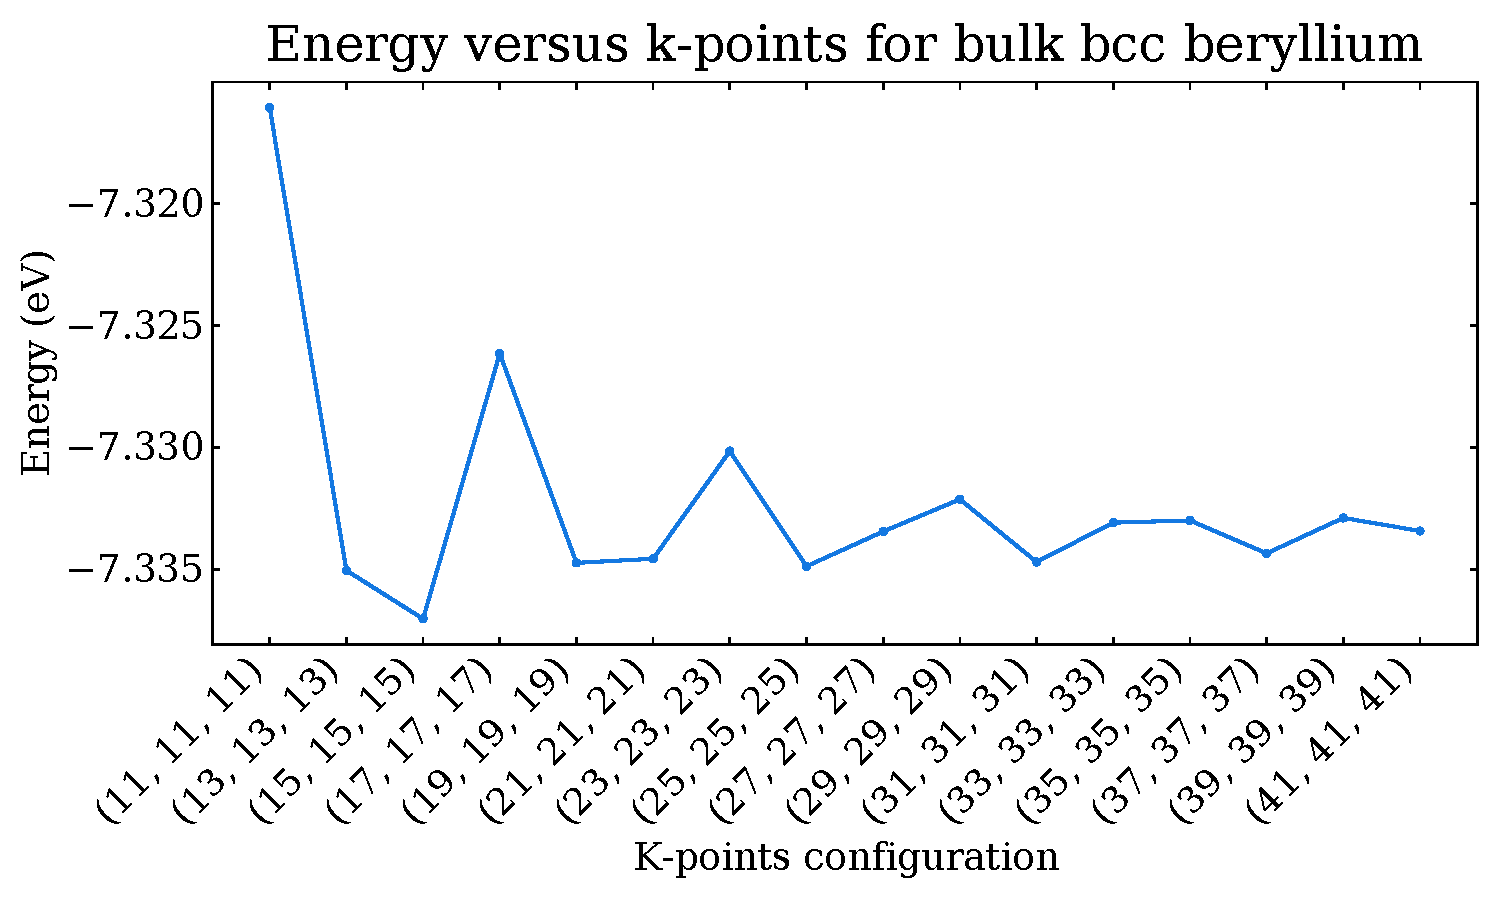
\includegraphics[width=0.40\linewidth]{figures_proj3/convergence_energy_kpoints_bcc-beryllium_thesis.pdf}&
    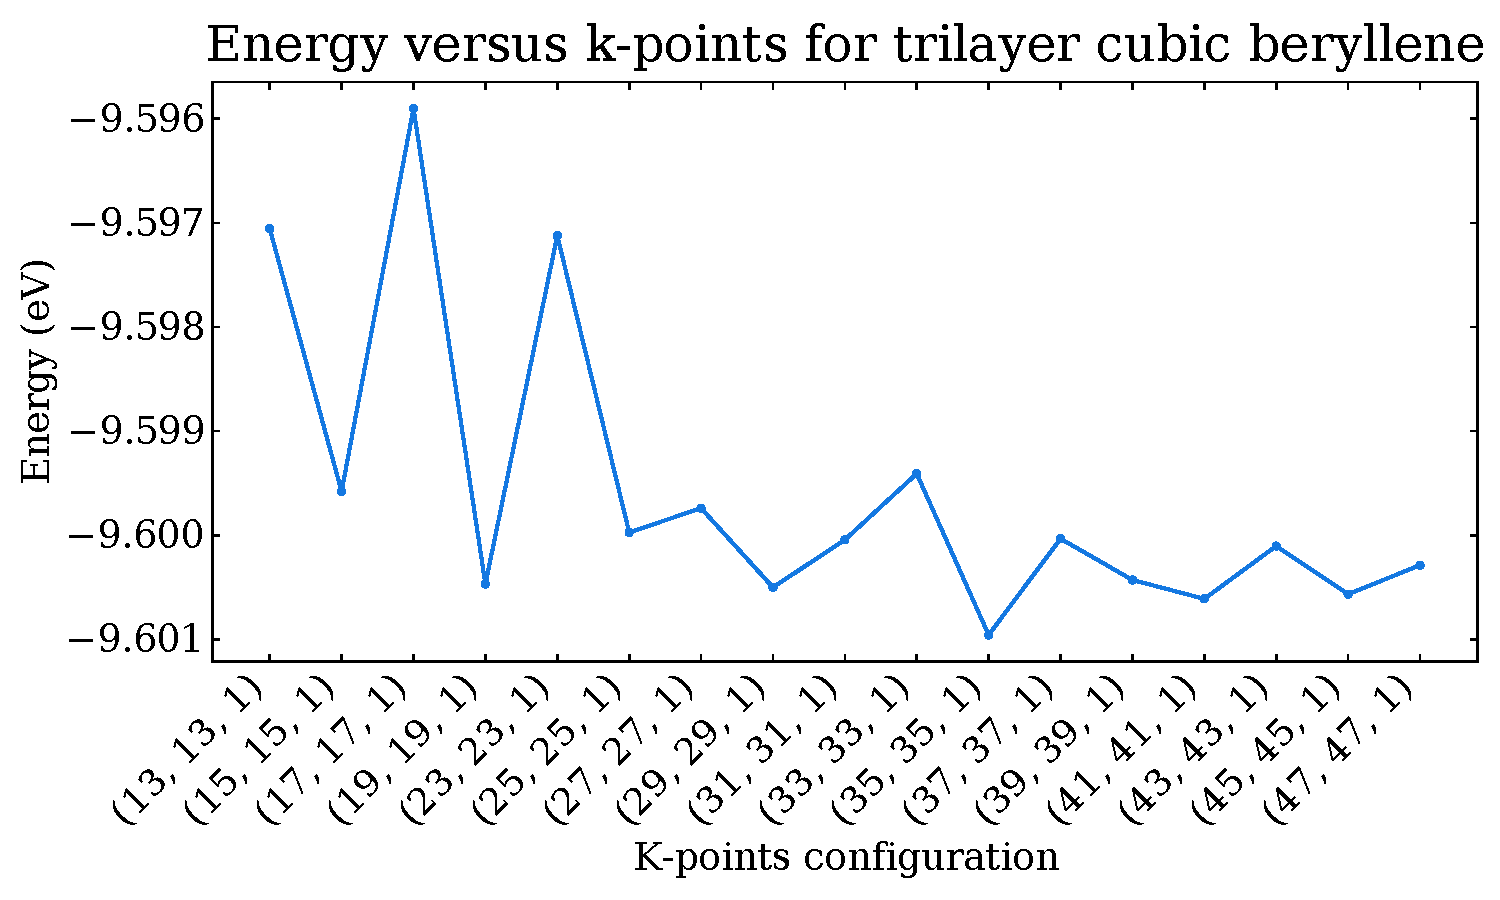
\includegraphics[width=0.40\linewidth]{figures_proj3/convergence_energy_kpoints_cubic-beryllene-trilayer_thesis.pdf}
\end{tabular}
\caption{Total energy as a function of k-point set for bulk hcp beryllium, $\alpha$-beryllene, bulk bcc beryllium, and trilayer cubic beryllene.}
\label{fig:proj3_total_energy_convergence}
\end{figure}

\subsection*{Optical-calculation parameters}

The dielectric function and the derived optical observables are introduced in chapter~\ref{cha:fundamentals_b},
especially section~\ref{sec:from_dielectric_function_to_optical_properties},
and the dielectric-function renormalization is given in equation~\eqref{optical_volume_normalization_2d}.
Therefore, we do not repeat these formula definitions here.
The structure thicknesses and the numbers of bands used in the optical calculations are specified below.

The effective thicknesses $d_{\mathrm{2D}}$ used in the dielectric-function renormalization are
\qty{3.960}{\angstrom} for pristine $\alpha$-beryllene,
\qty{5.869}{\angstrom} for pristine $\beta$-beryllene,
\qty{6.966}{\angstrom} for trilayer cubic beryllene,
\qty{3.145}{\angstrom} for 2H-$\alpha$-beryllene,
\qty{5.524}{\angstrom} for 1H-$\beta$-beryllene,
and \qty{5.193}{\angstrom} for 2H-$\beta$-beryllene.
We assign $d_{\mathrm{2D}}$ as the separation of the outermost atomic centres along the surface normal,
plus the radii of the atoms at those two surfaces: \qty{1.98}{\angstrom} for Be and \qty{0.70}{\angstrom} for H.
The relaxed coordinates are converted to Cartesian lengths with periodic wrapping removed.
The same optical volume normalization is applied to the $xx$, $yy$ and $zz$ components.
The absolute effective response depends on this thickness convention.
The endpoint-radius contribution is Be+Be for pristine structures, H+H for double-sided termination, and Be+H for single-sided termination.
Consequently, the assigned 2H-$\alpha$ thickness is smaller than the pristine value; this is a consequence of the chosen convention and is not a unique physical layer thickness.
Unrounded structure-derived values are used in all calculations.
The actual total numbers of bands are 140 for each hydrogenated structure,
133 for pristine $\alpha$-beryllene and trilayer cubic beryllene,
128 for pristine $\beta$-beryllene,
70 for bulk bcc beryllium and 66 for bulk hcp beryllium.
These are total bands, not counts of unoccupied bands; the actual output may differ from the requested \texttt{NBANDS} because of parallel band allocation.

\subsection*{Dielectric-function convergence}

The convergence of the calculated dielectric function is examined with respect to the number of bands included in the calculation and the k-point set.
Figures~\ref{fig:proj3_hcp_dielectric_nbands_convergence}--\ref{fig:proj3_cubic_dielectric_kpoint_convergence}
show the corresponding tests for bulk hcp beryllium,
$\alpha$-beryllene, $\beta$-beryllene, bulk bcc beryllium,
and trilayer cubic beryllene.
The plots retain the full range of every curve within the displayed energy window.
In particular, the bulk hcp $45\times45\times45$ k-point calculation has a large low-energy dielectric response that is visible in figure~\ref{fig:proj3_hcp_dielectric_kpoint_convergence}.
These comparisons do not establish convergence of the complete low-frequency metallic response, which would also require an intraband treatment.
The selected reference may change both the k-point grid and the total band count relative to a convergence series;
it is a final-parameter reference rather than an additional strictly one-parameter convergence point.

\begin{figure}[!htbp]
\centering
    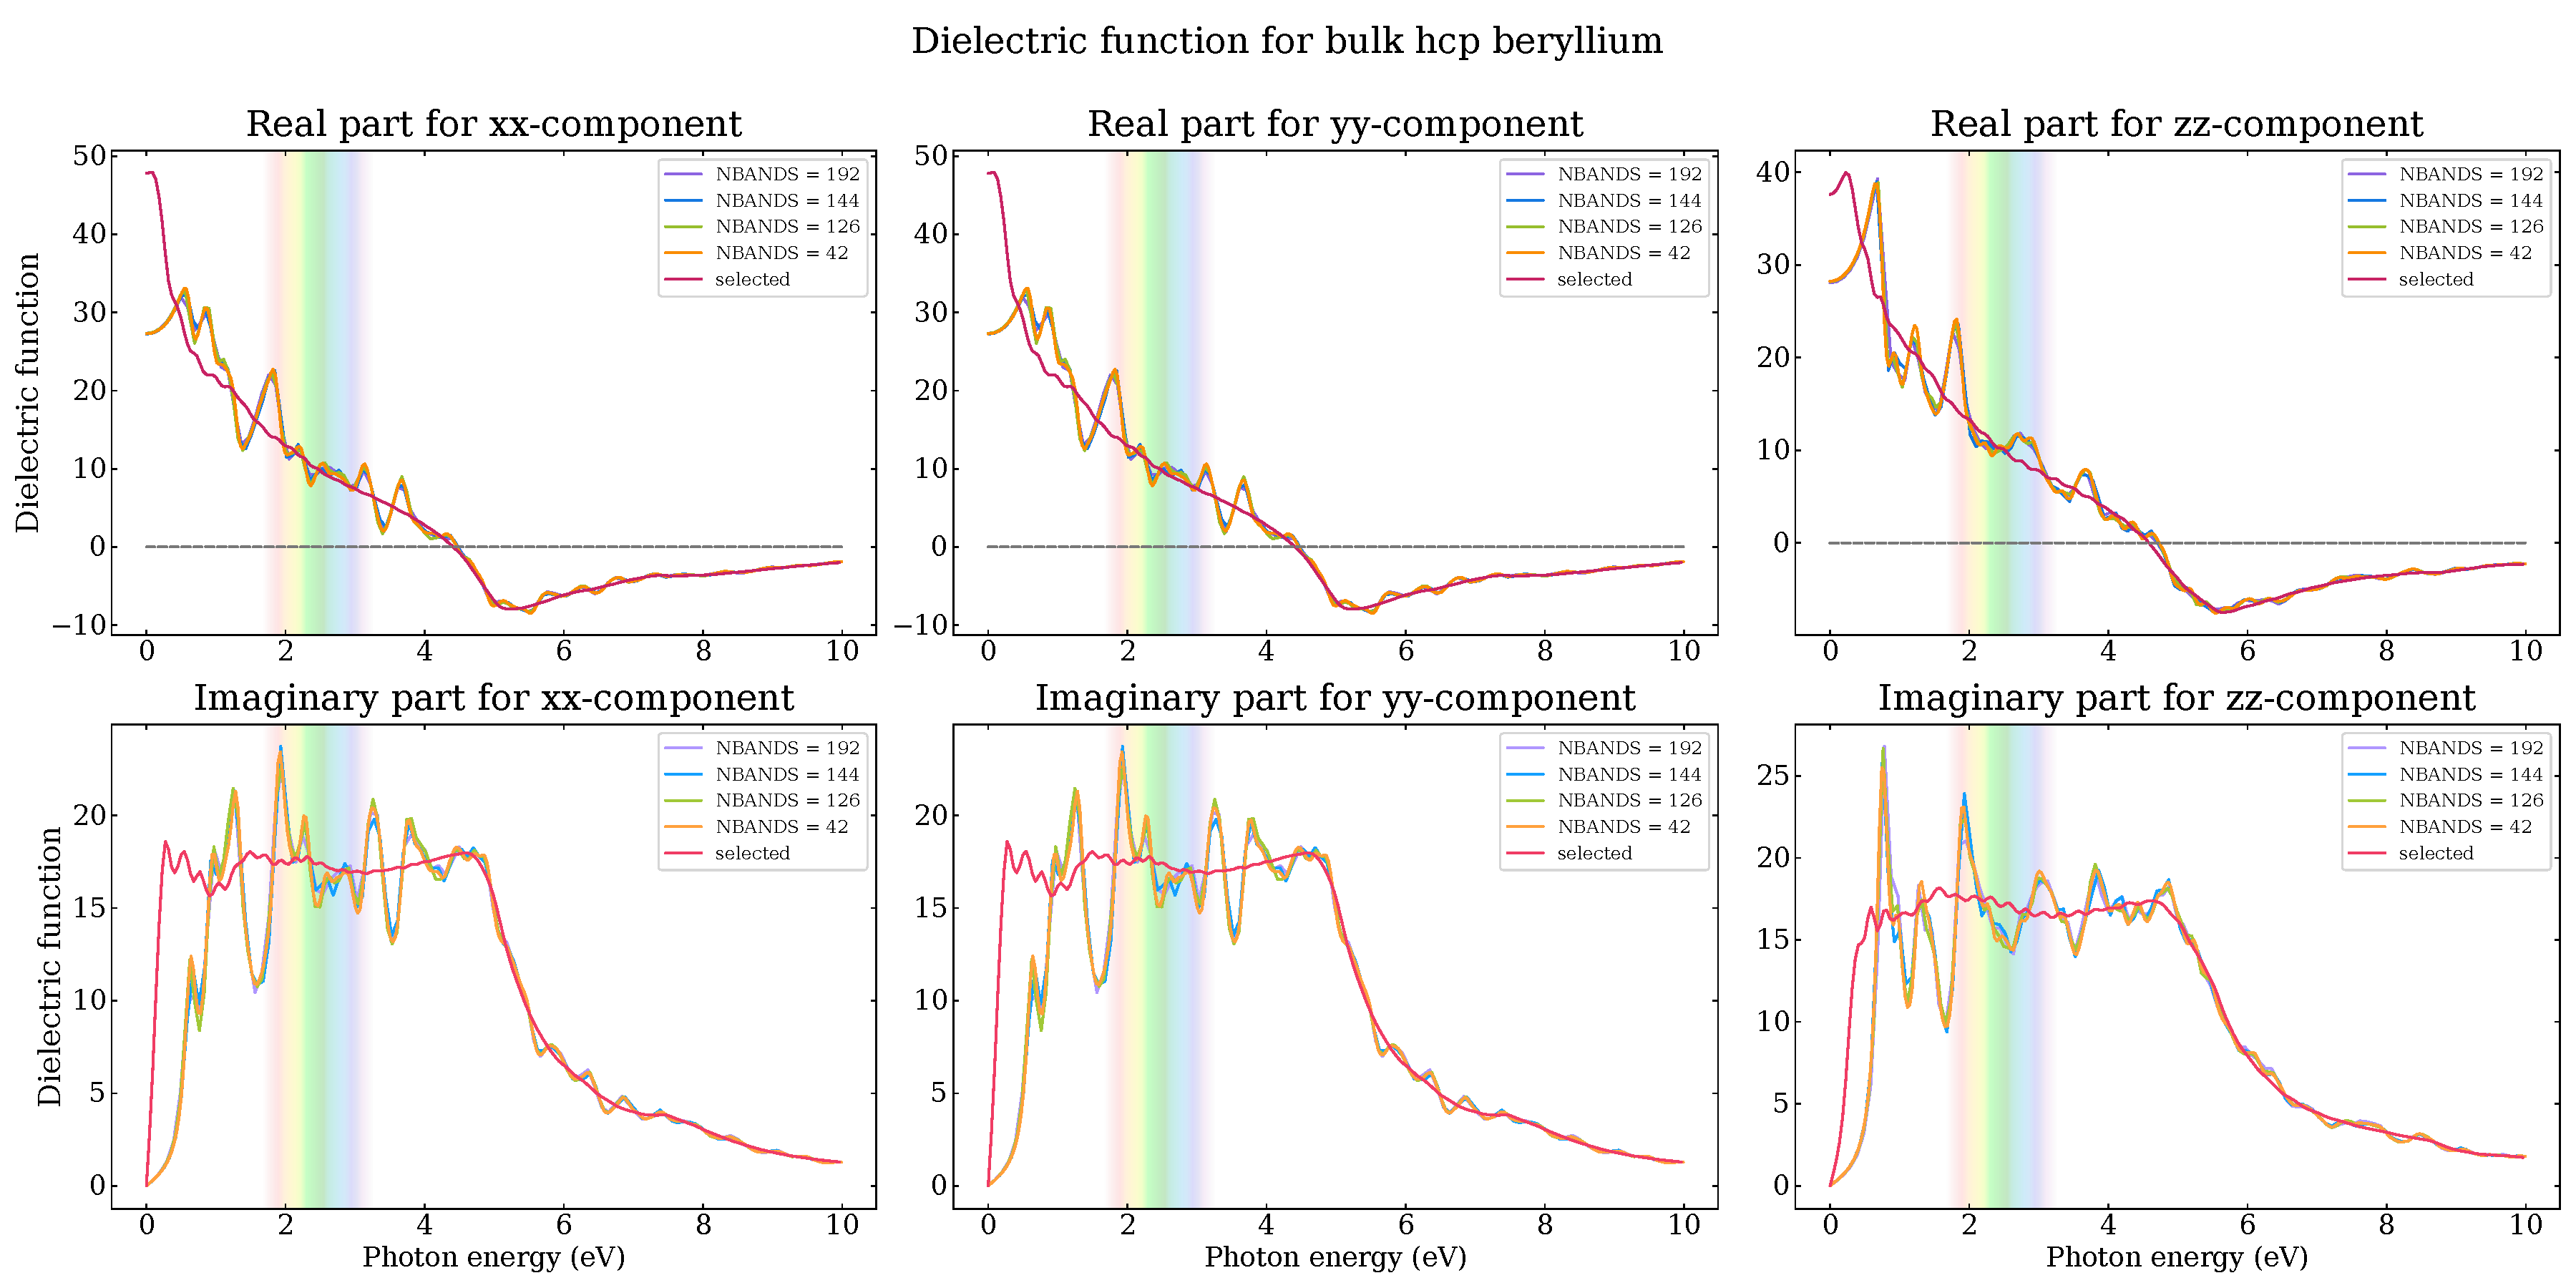
\includegraphics[width=1.0\linewidth]{figures_proj3/convergence_dielectric_nbands_hcp-beryllium_thesis.pdf}
\caption{Real and imaginary parts of the dielectric function for bulk hcp beryllium,
calculated with different total numbers of bands included in the calculation.}
\label{fig:proj3_hcp_dielectric_nbands_convergence}
\end{figure}

\begin{figure}[!htbp]
\centering
    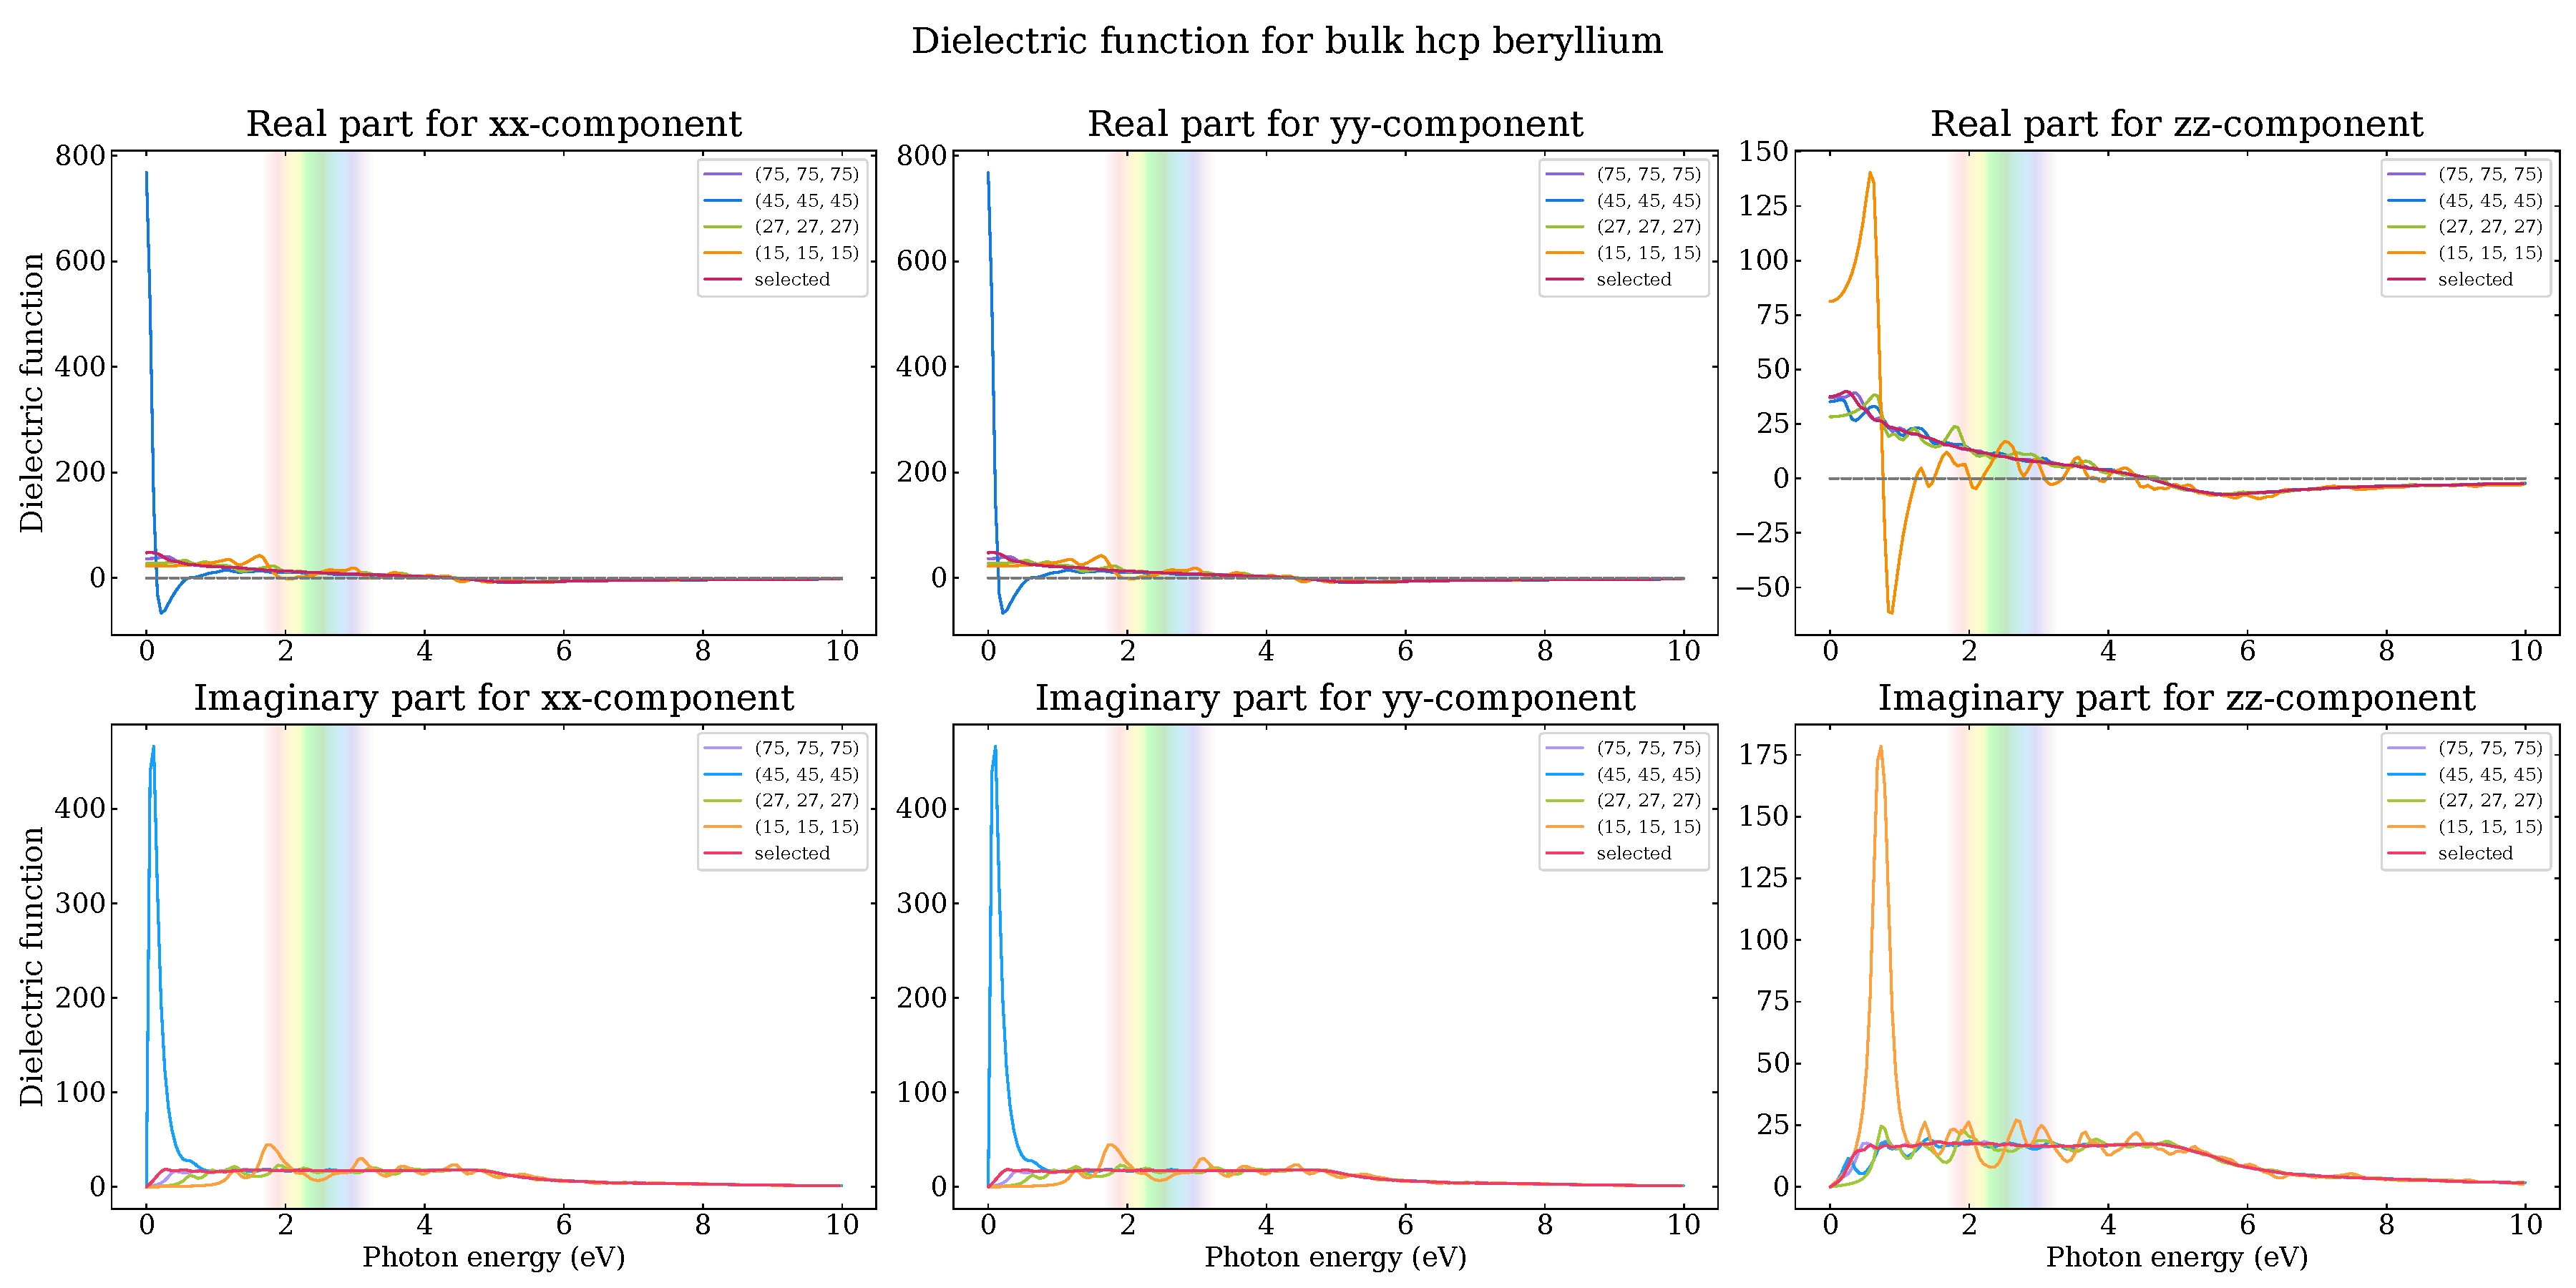
\includegraphics[width=1.0\linewidth]{figures_proj3/convergence_dielectric_kpoints_hcp-beryllium_thesis.pdf}
\caption{Real and imaginary parts of the dielectric function for bulk hcp beryllium,
calculated with different k-point sets.}
\label{fig:proj3_hcp_dielectric_kpoint_convergence}
\end{figure}

\begin{figure}[!htbp]
\centering
    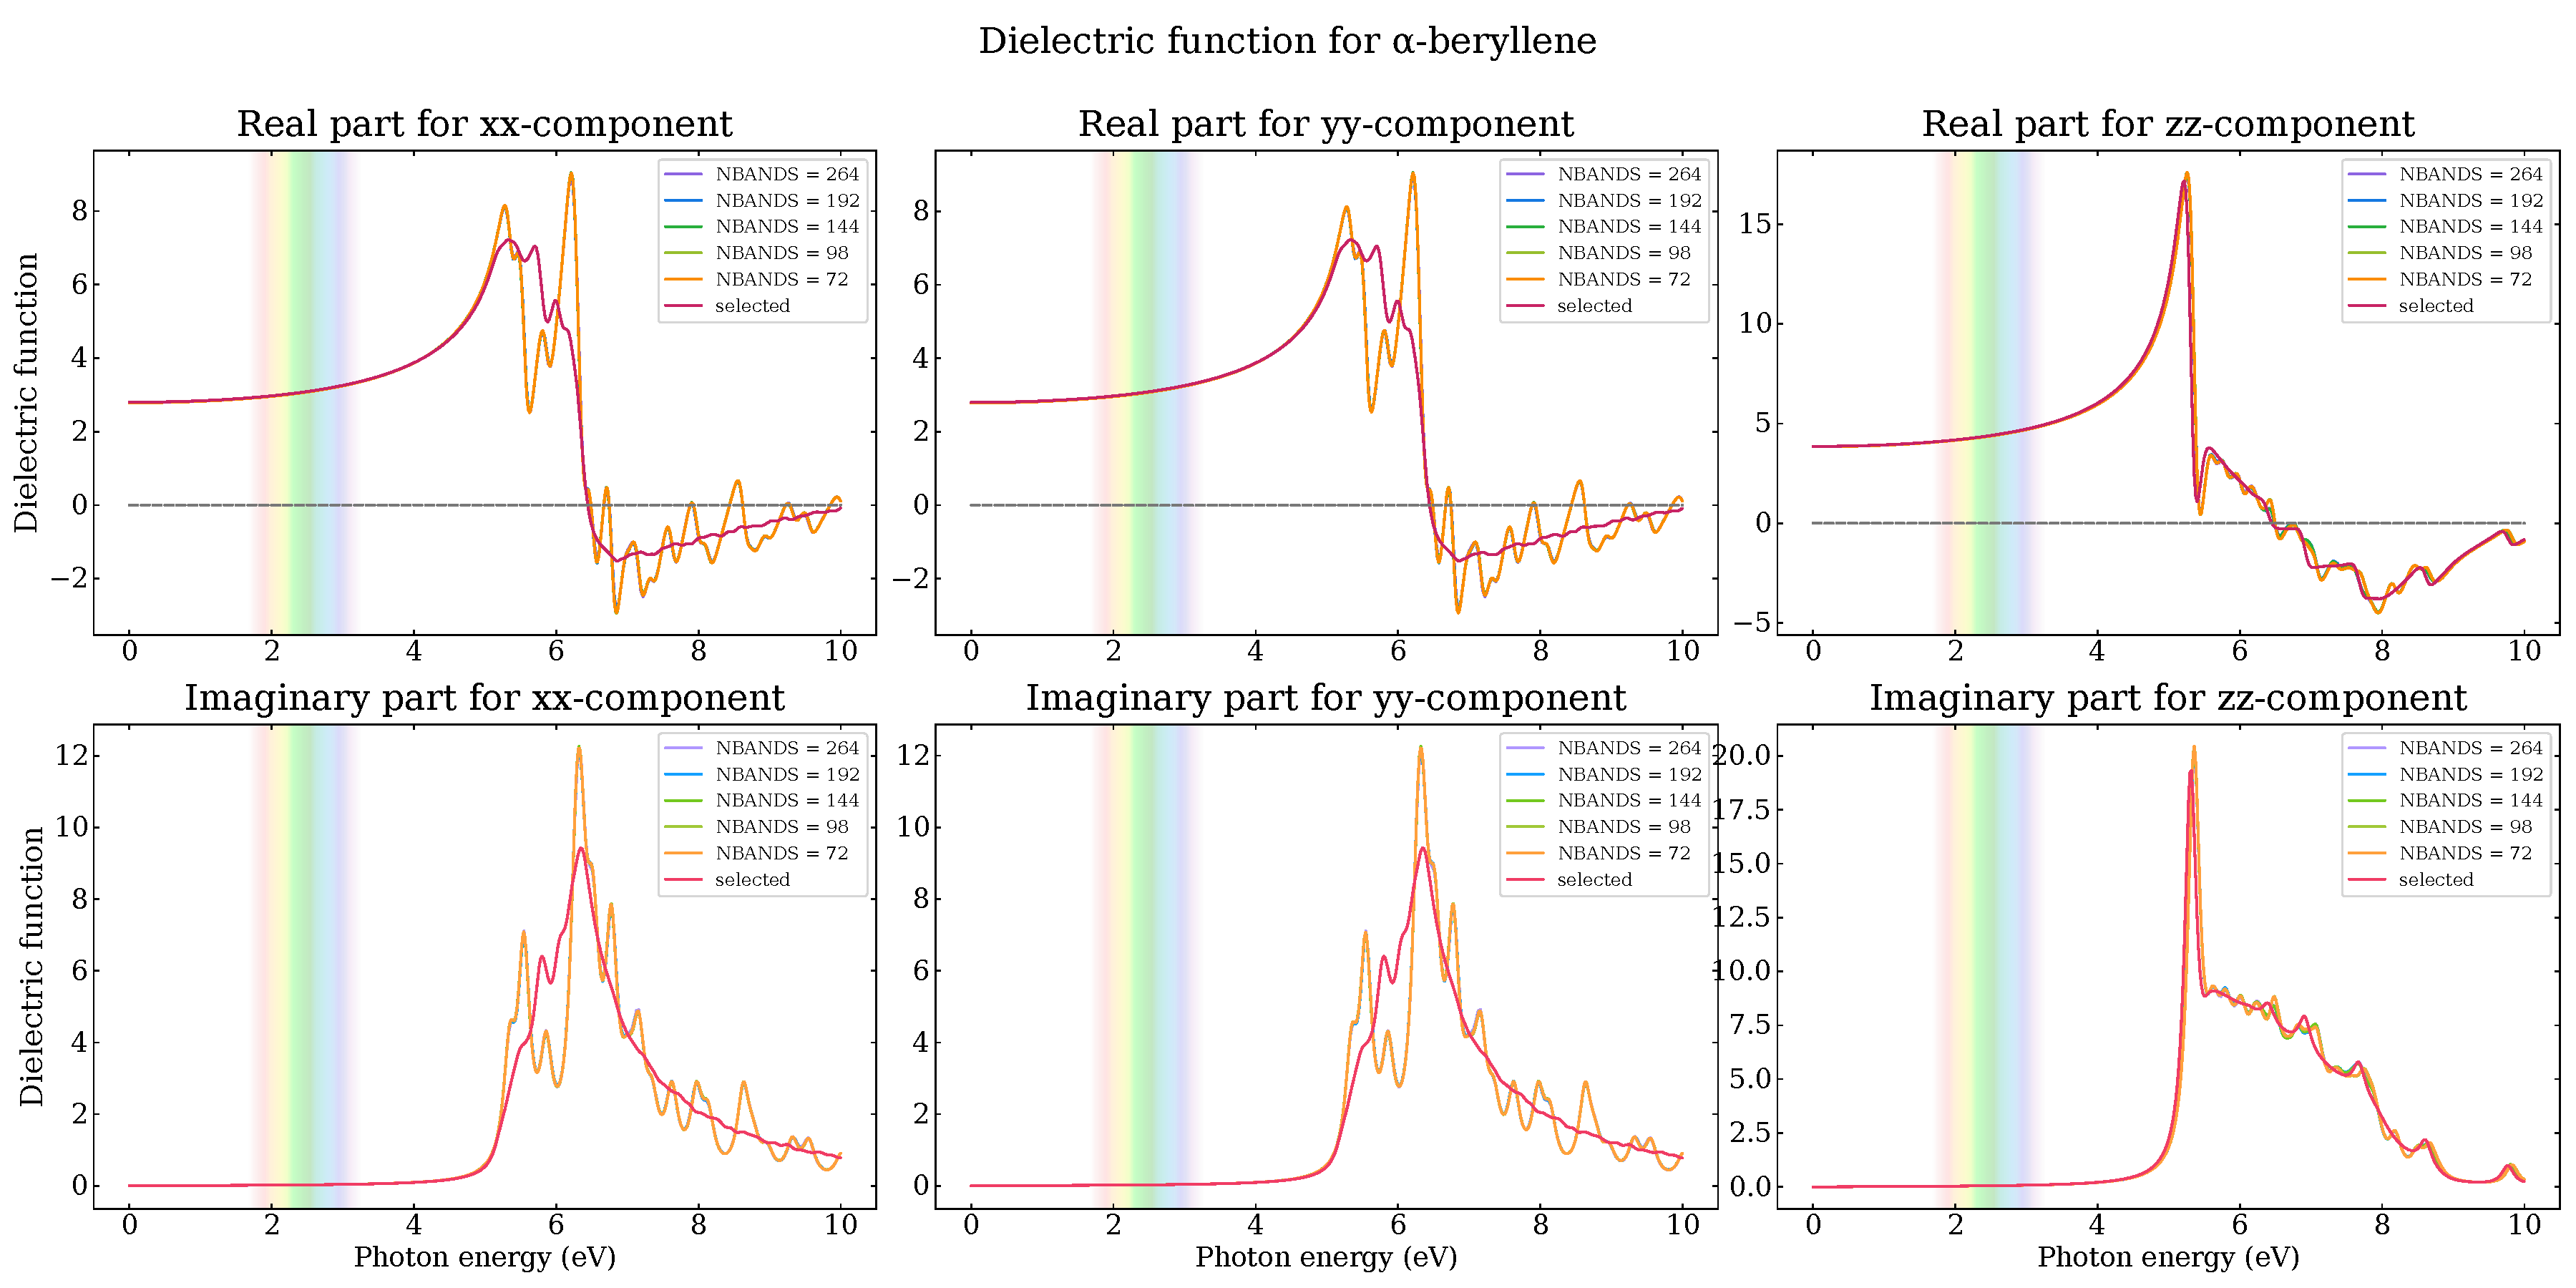
\includegraphics[width=1.0\linewidth]{figures_proj3/convergence_dielectric_nbands_alpha-beryllene_thesis.pdf}
\caption{Real and imaginary parts of the dielectric function for $\alpha$-beryllene,
calculated with different total numbers of bands included in the calculation.}
\label{fig:proj3_alpha_dielectric_nbands_convergence}
\end{figure}

\begin{figure}[!htbp]
\centering
    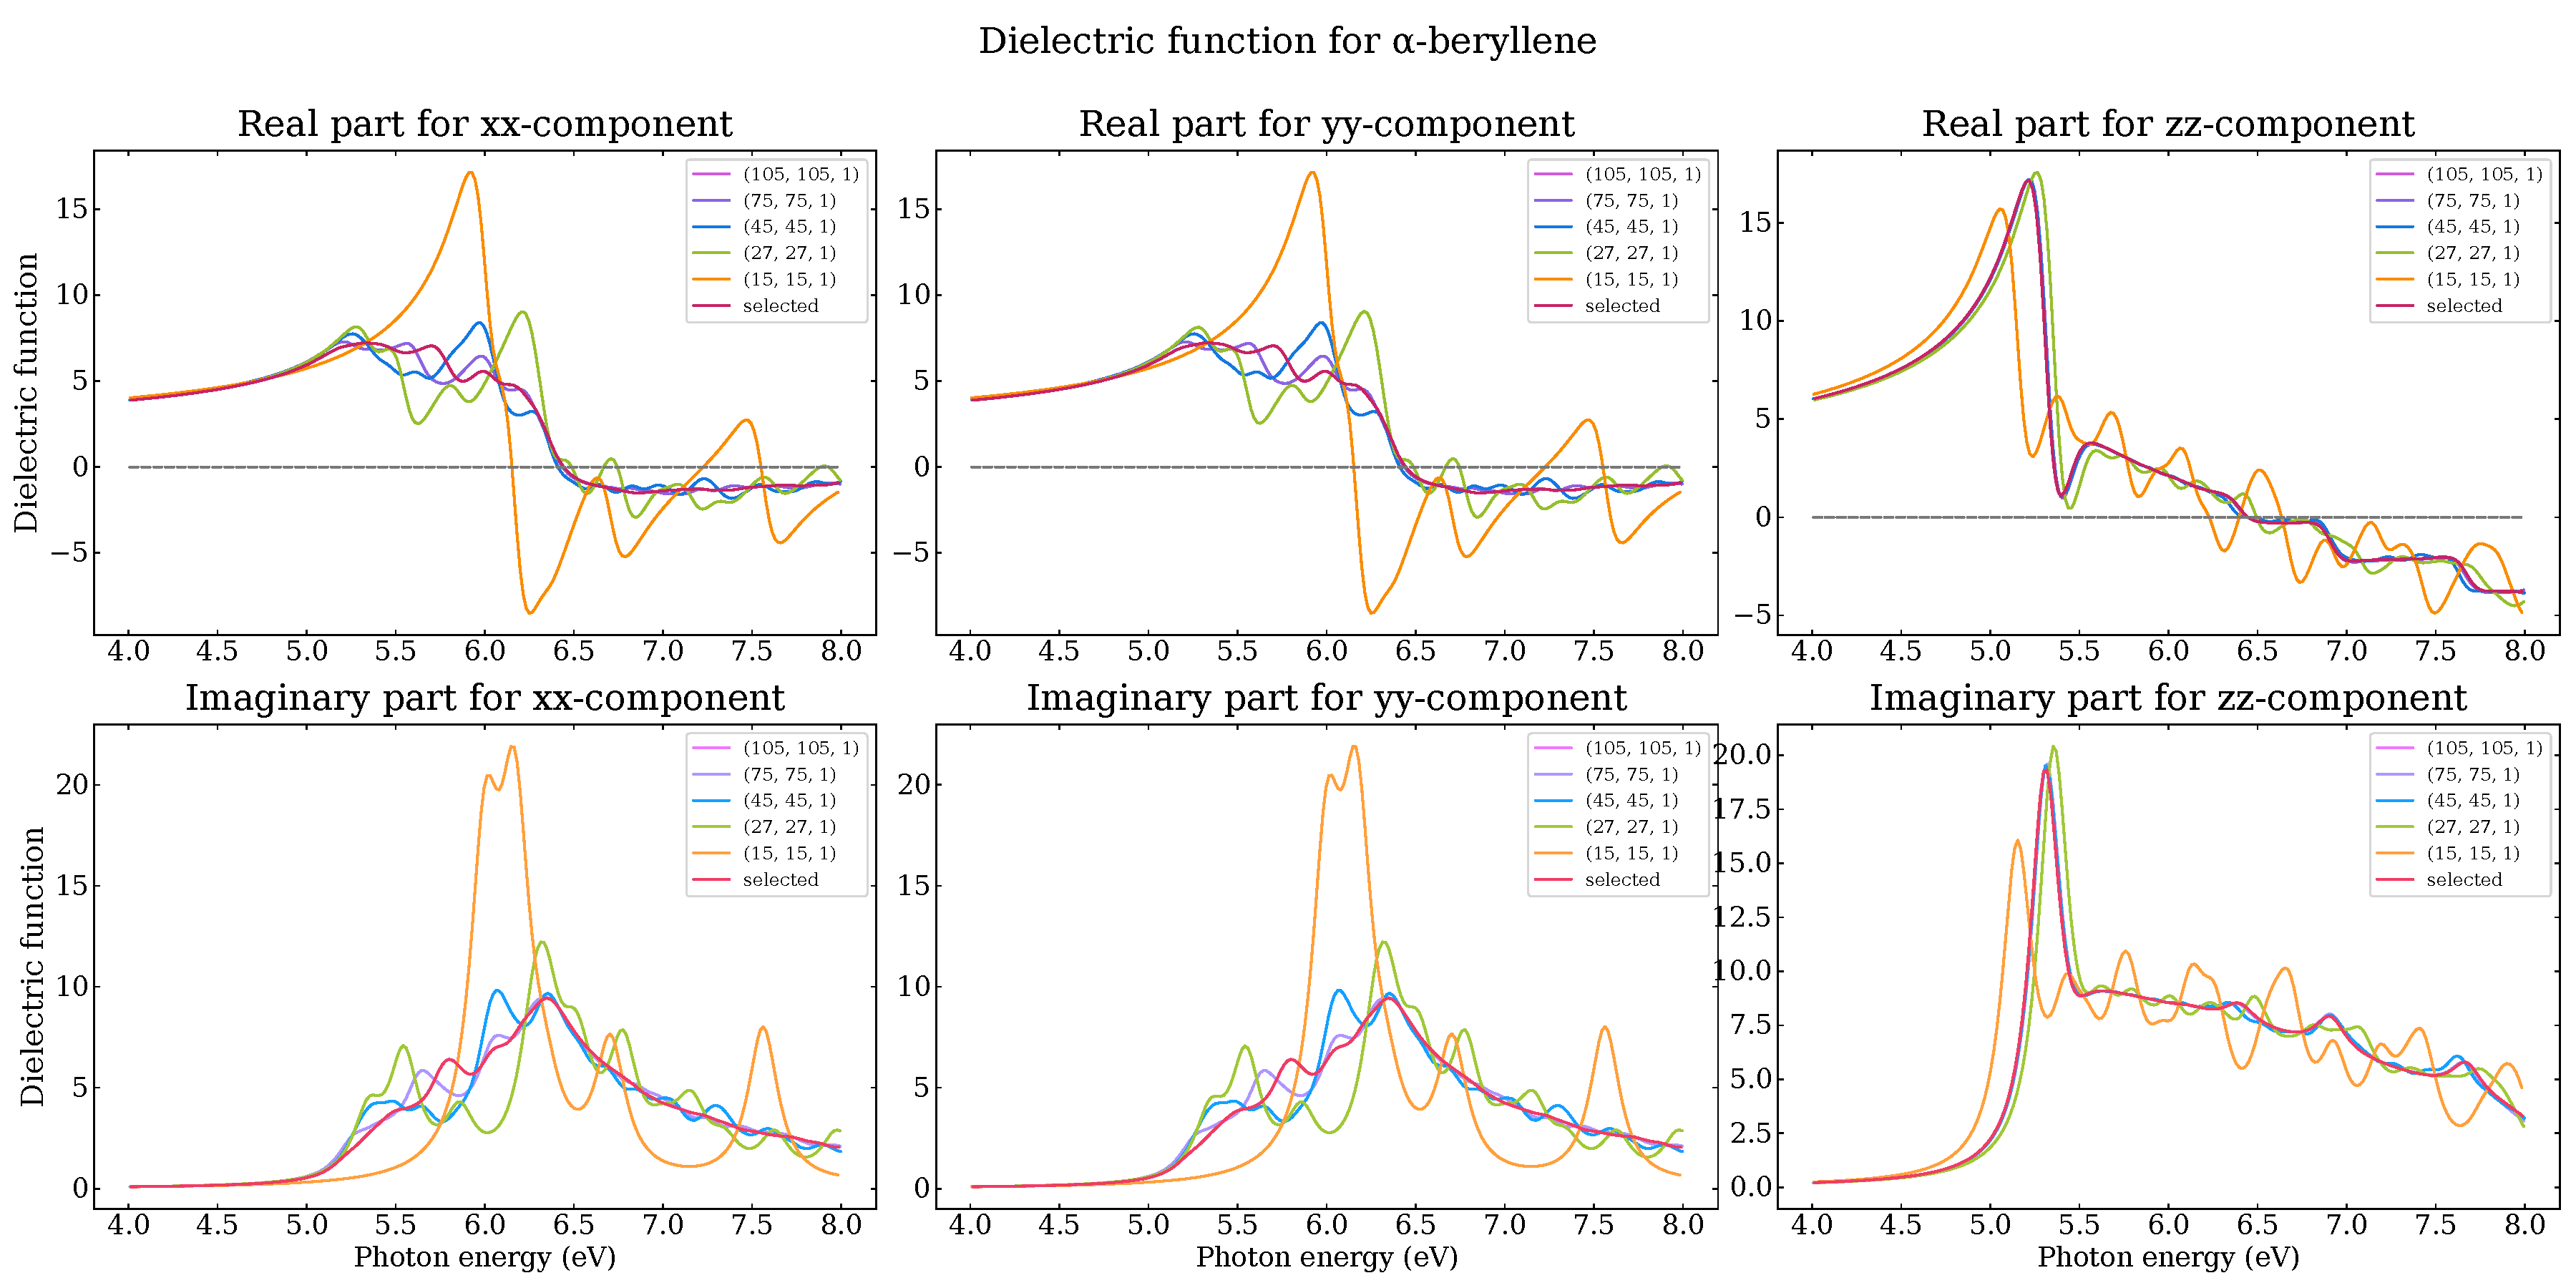
\includegraphics[width=1.0\linewidth]{figures_proj3/convergence_dielectric_kpoints_alpha-beryllene_thesis.pdf}
\caption{Real and imaginary parts of the dielectric function for $\alpha$-beryllene,
calculated with different k-point sets.}
\label{fig:proj3_alpha_dielectric_kpoint_convergence}
\end{figure}

\begin{figure}[!htbp]
\centering
    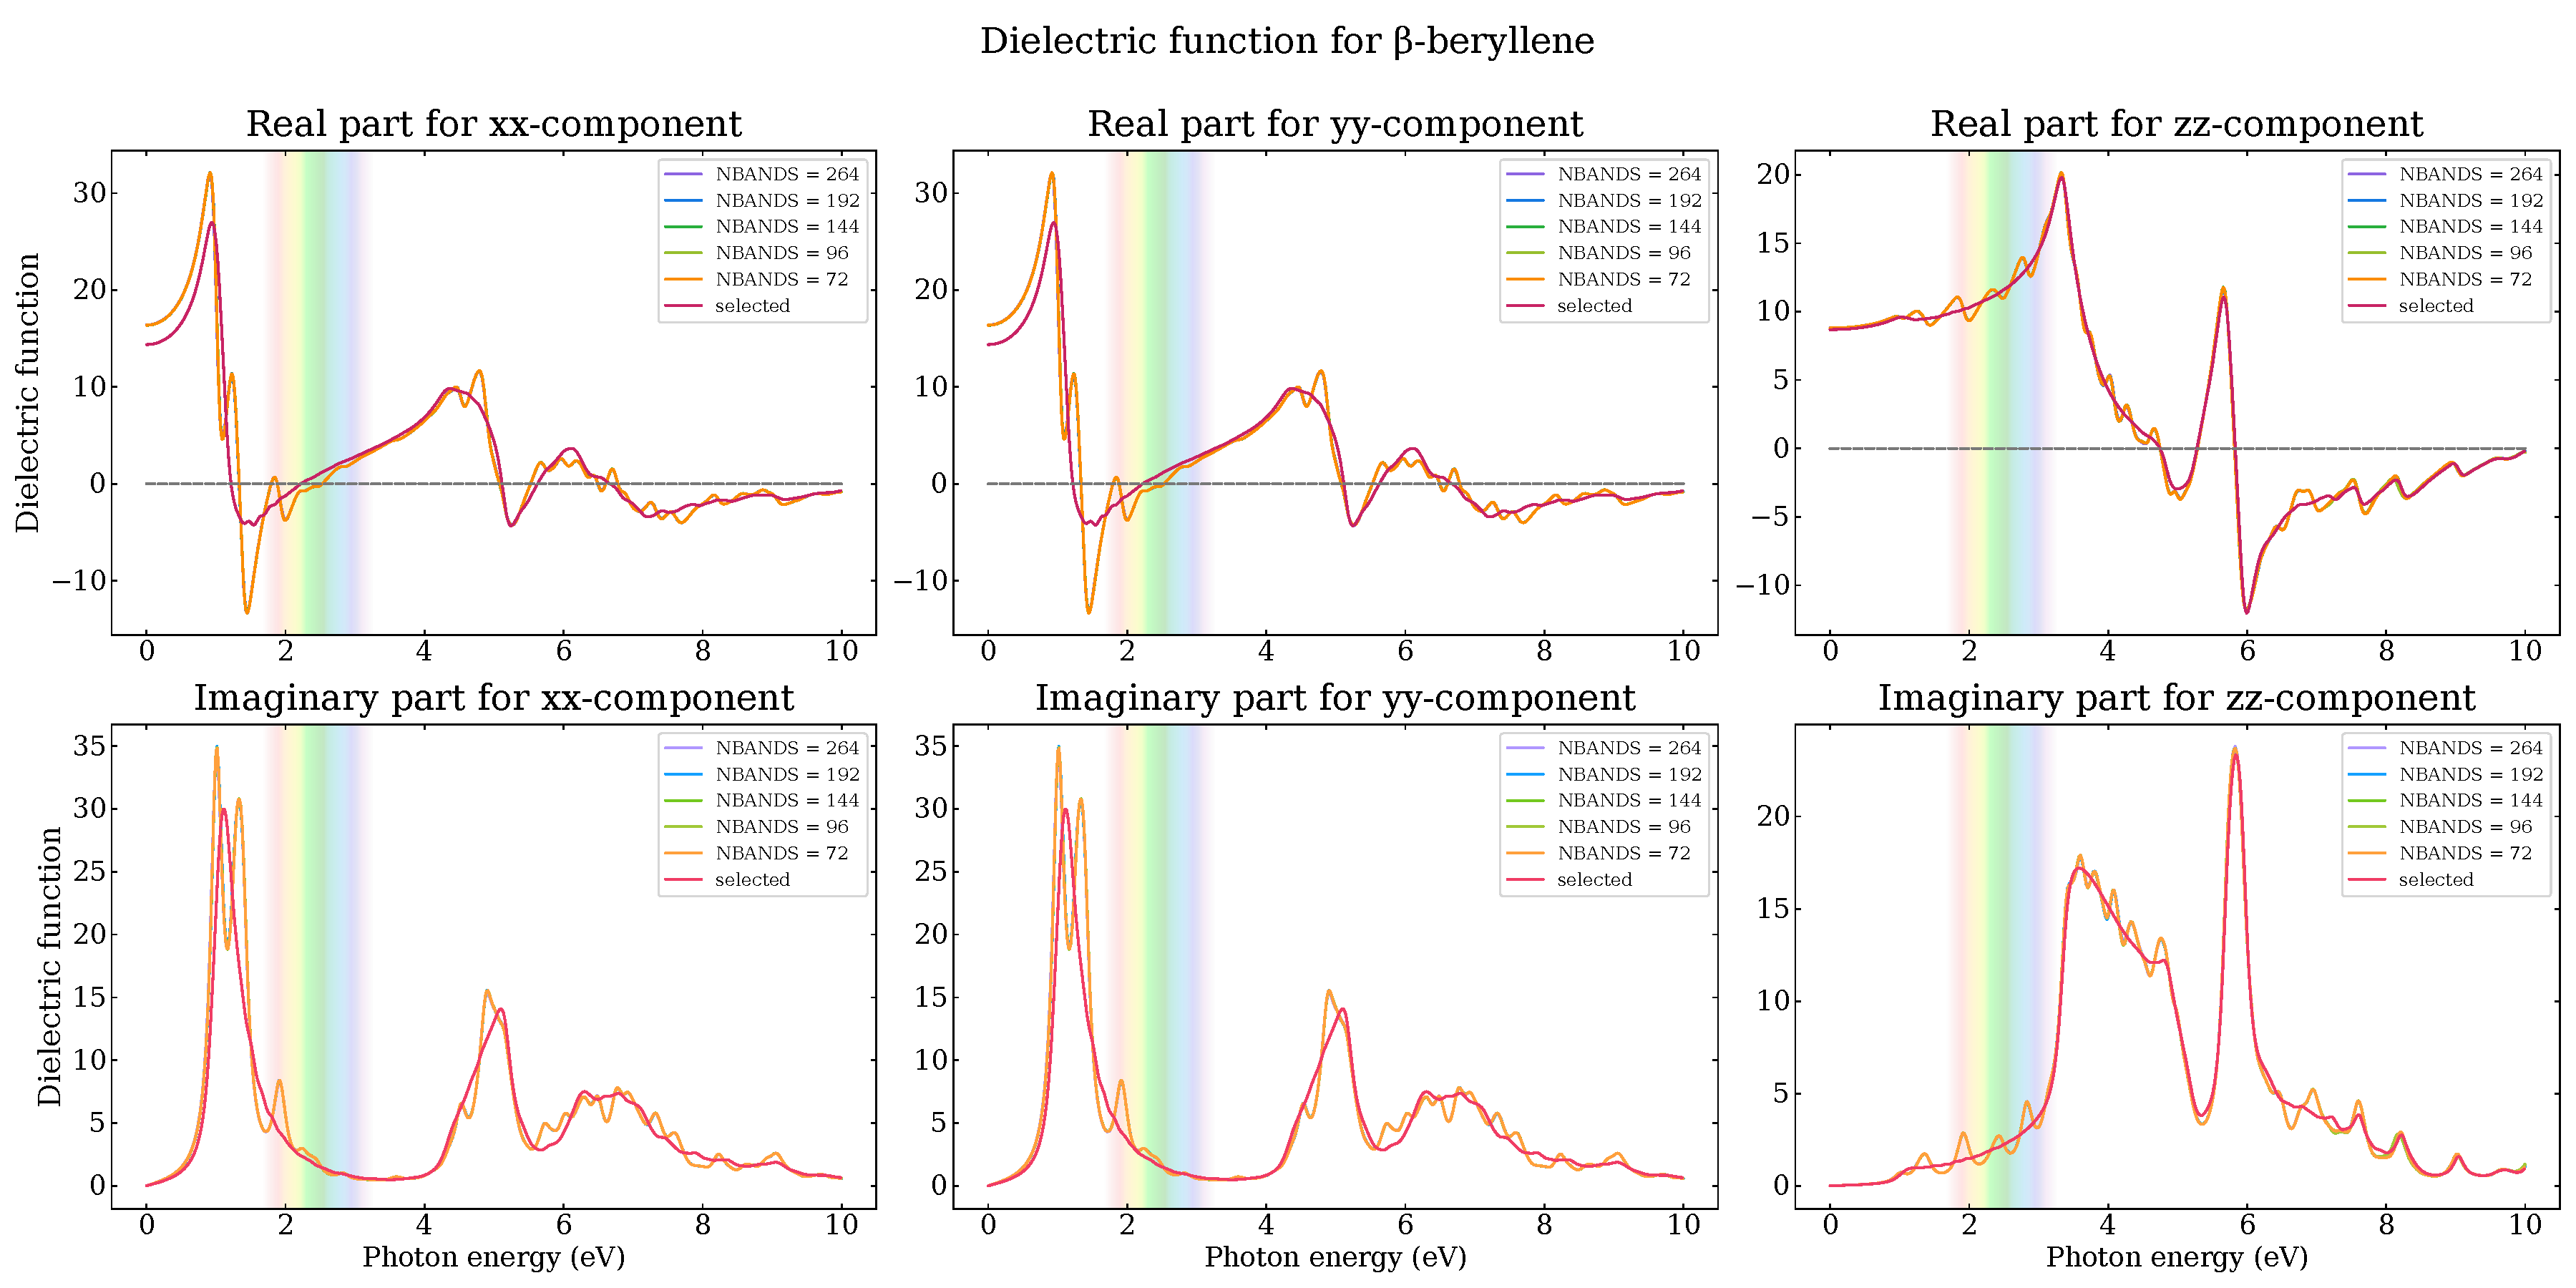
\includegraphics[width=1.0\linewidth]{figures_proj3/convergence_dielectric_nbands_beta-beryllene_thesis.pdf}
\caption{Real and imaginary parts of the dielectric function for $\beta$-beryllene,
calculated with different total numbers of bands included in the calculation.}
\label{fig:proj3_beta_dielectric_nbands_convergence}
\end{figure}

\begin{figure}[!htbp]
\centering
    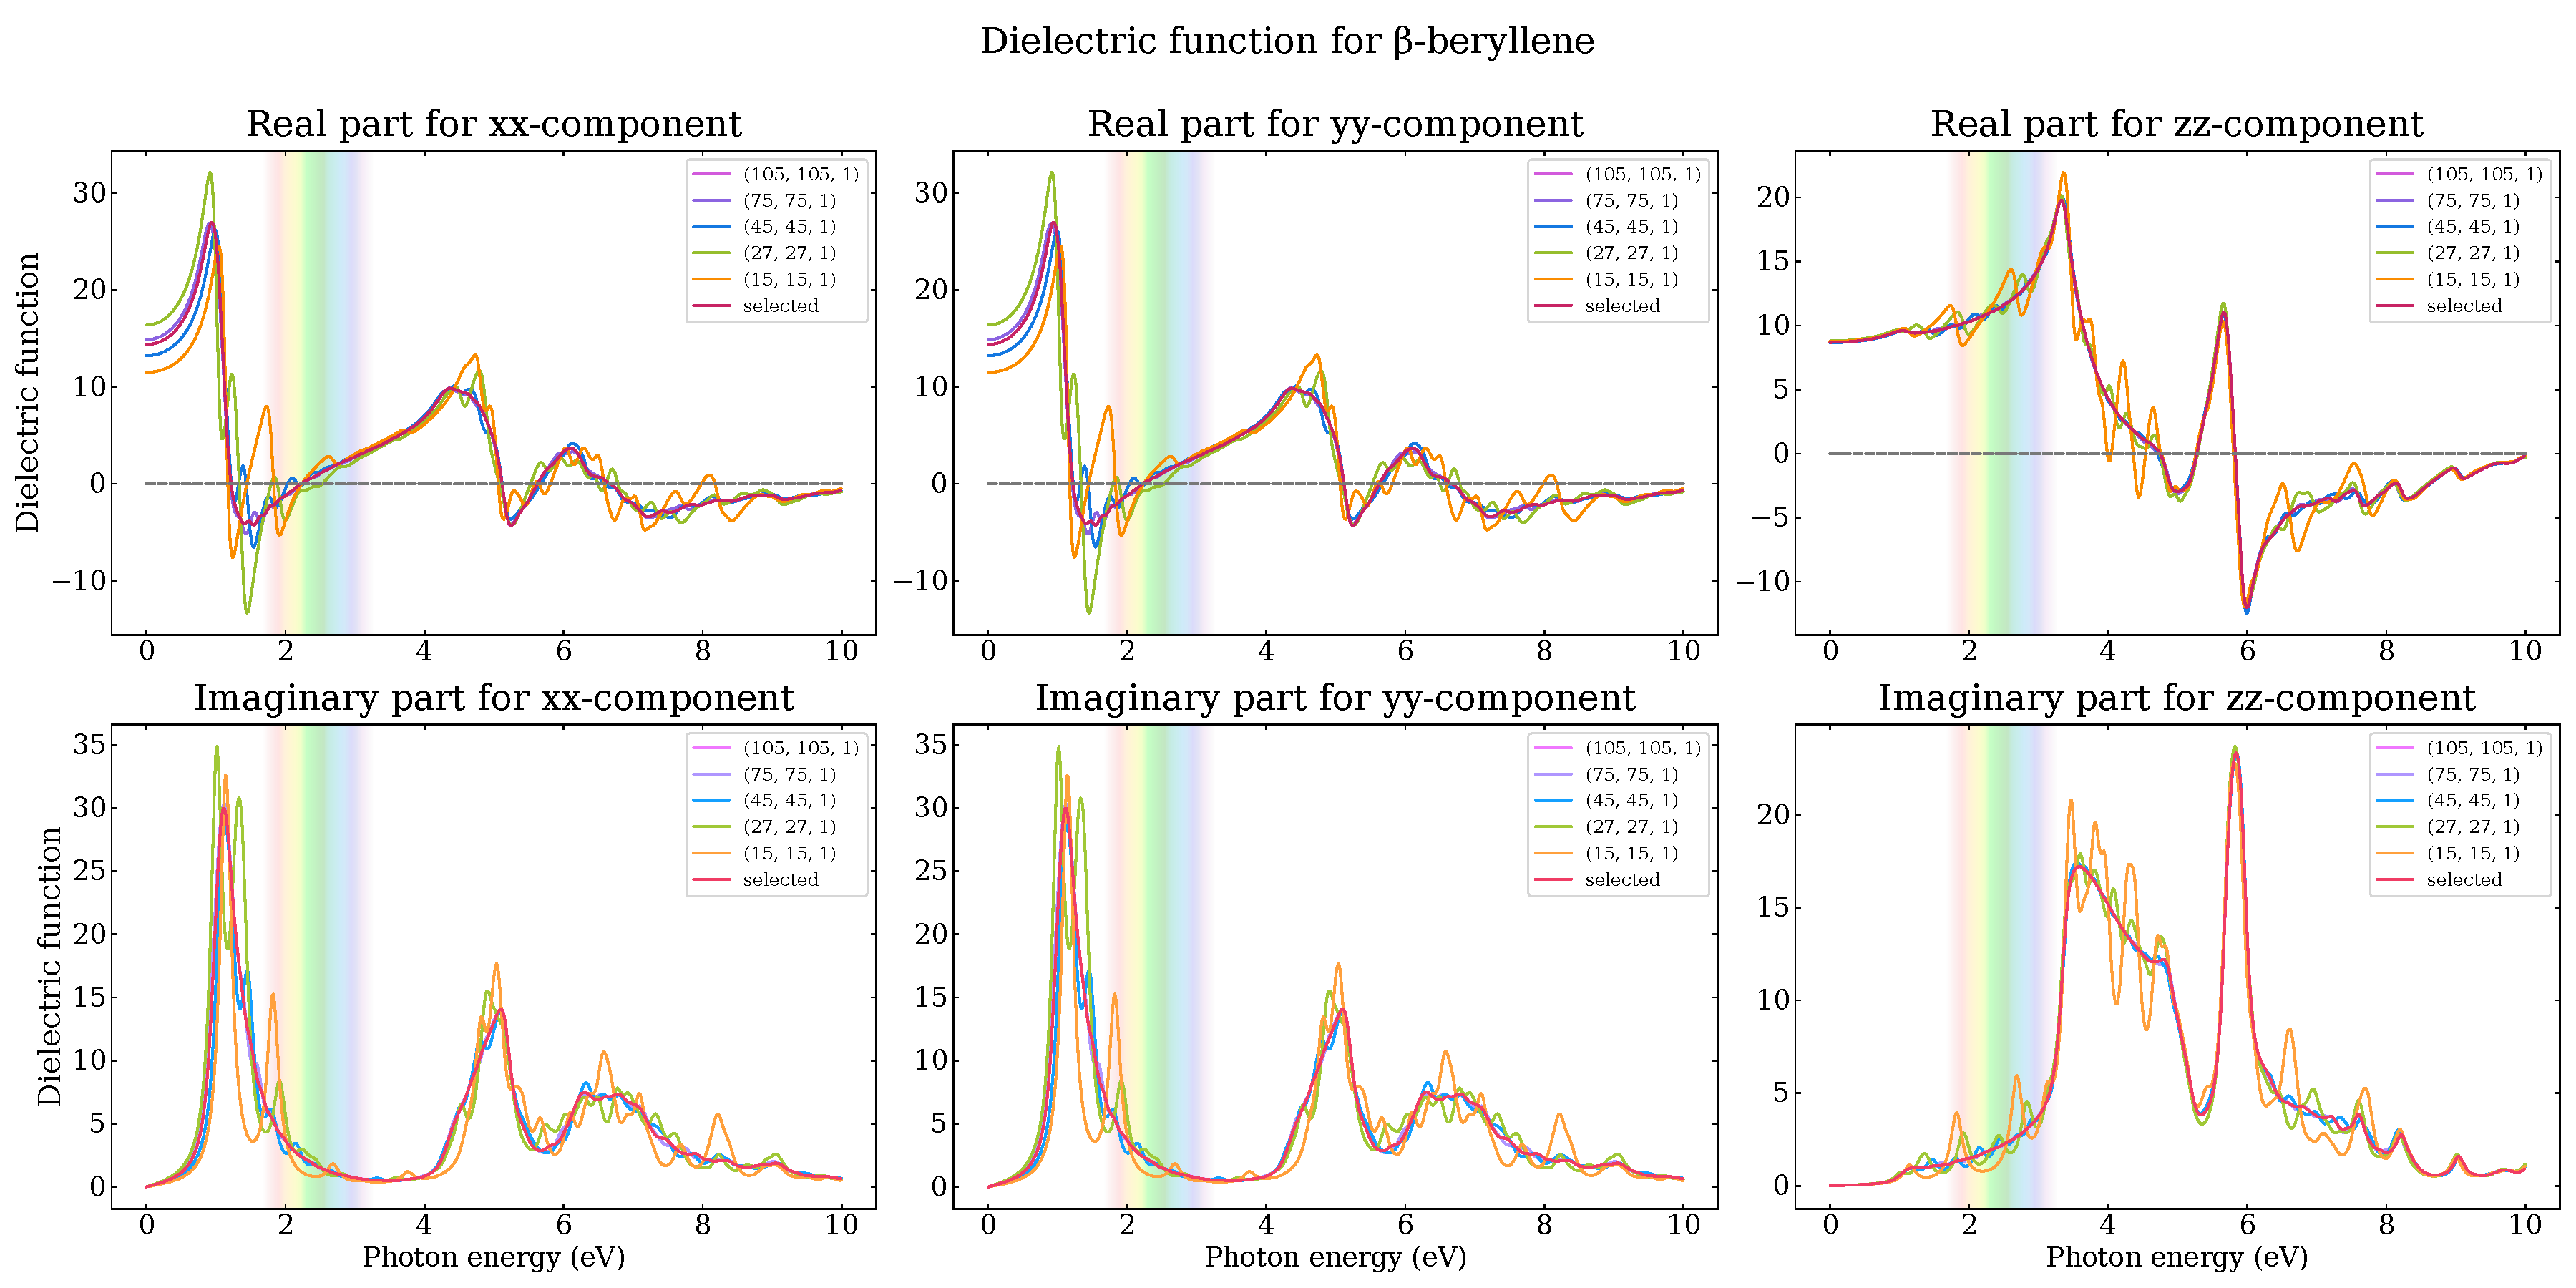
\includegraphics[width=1.0\linewidth]{figures_proj3/convergence_dielectric_kpoints_beta-beryllene_thesis.pdf}
\caption{Real and imaginary parts of the dielectric function for $\beta$-beryllene,
calculated with different k-point sets.}
\label{fig:proj3_beta_dielectric_kpoint_convergence}
\end{figure}

\begin{figure}[!htbp]
\centering
    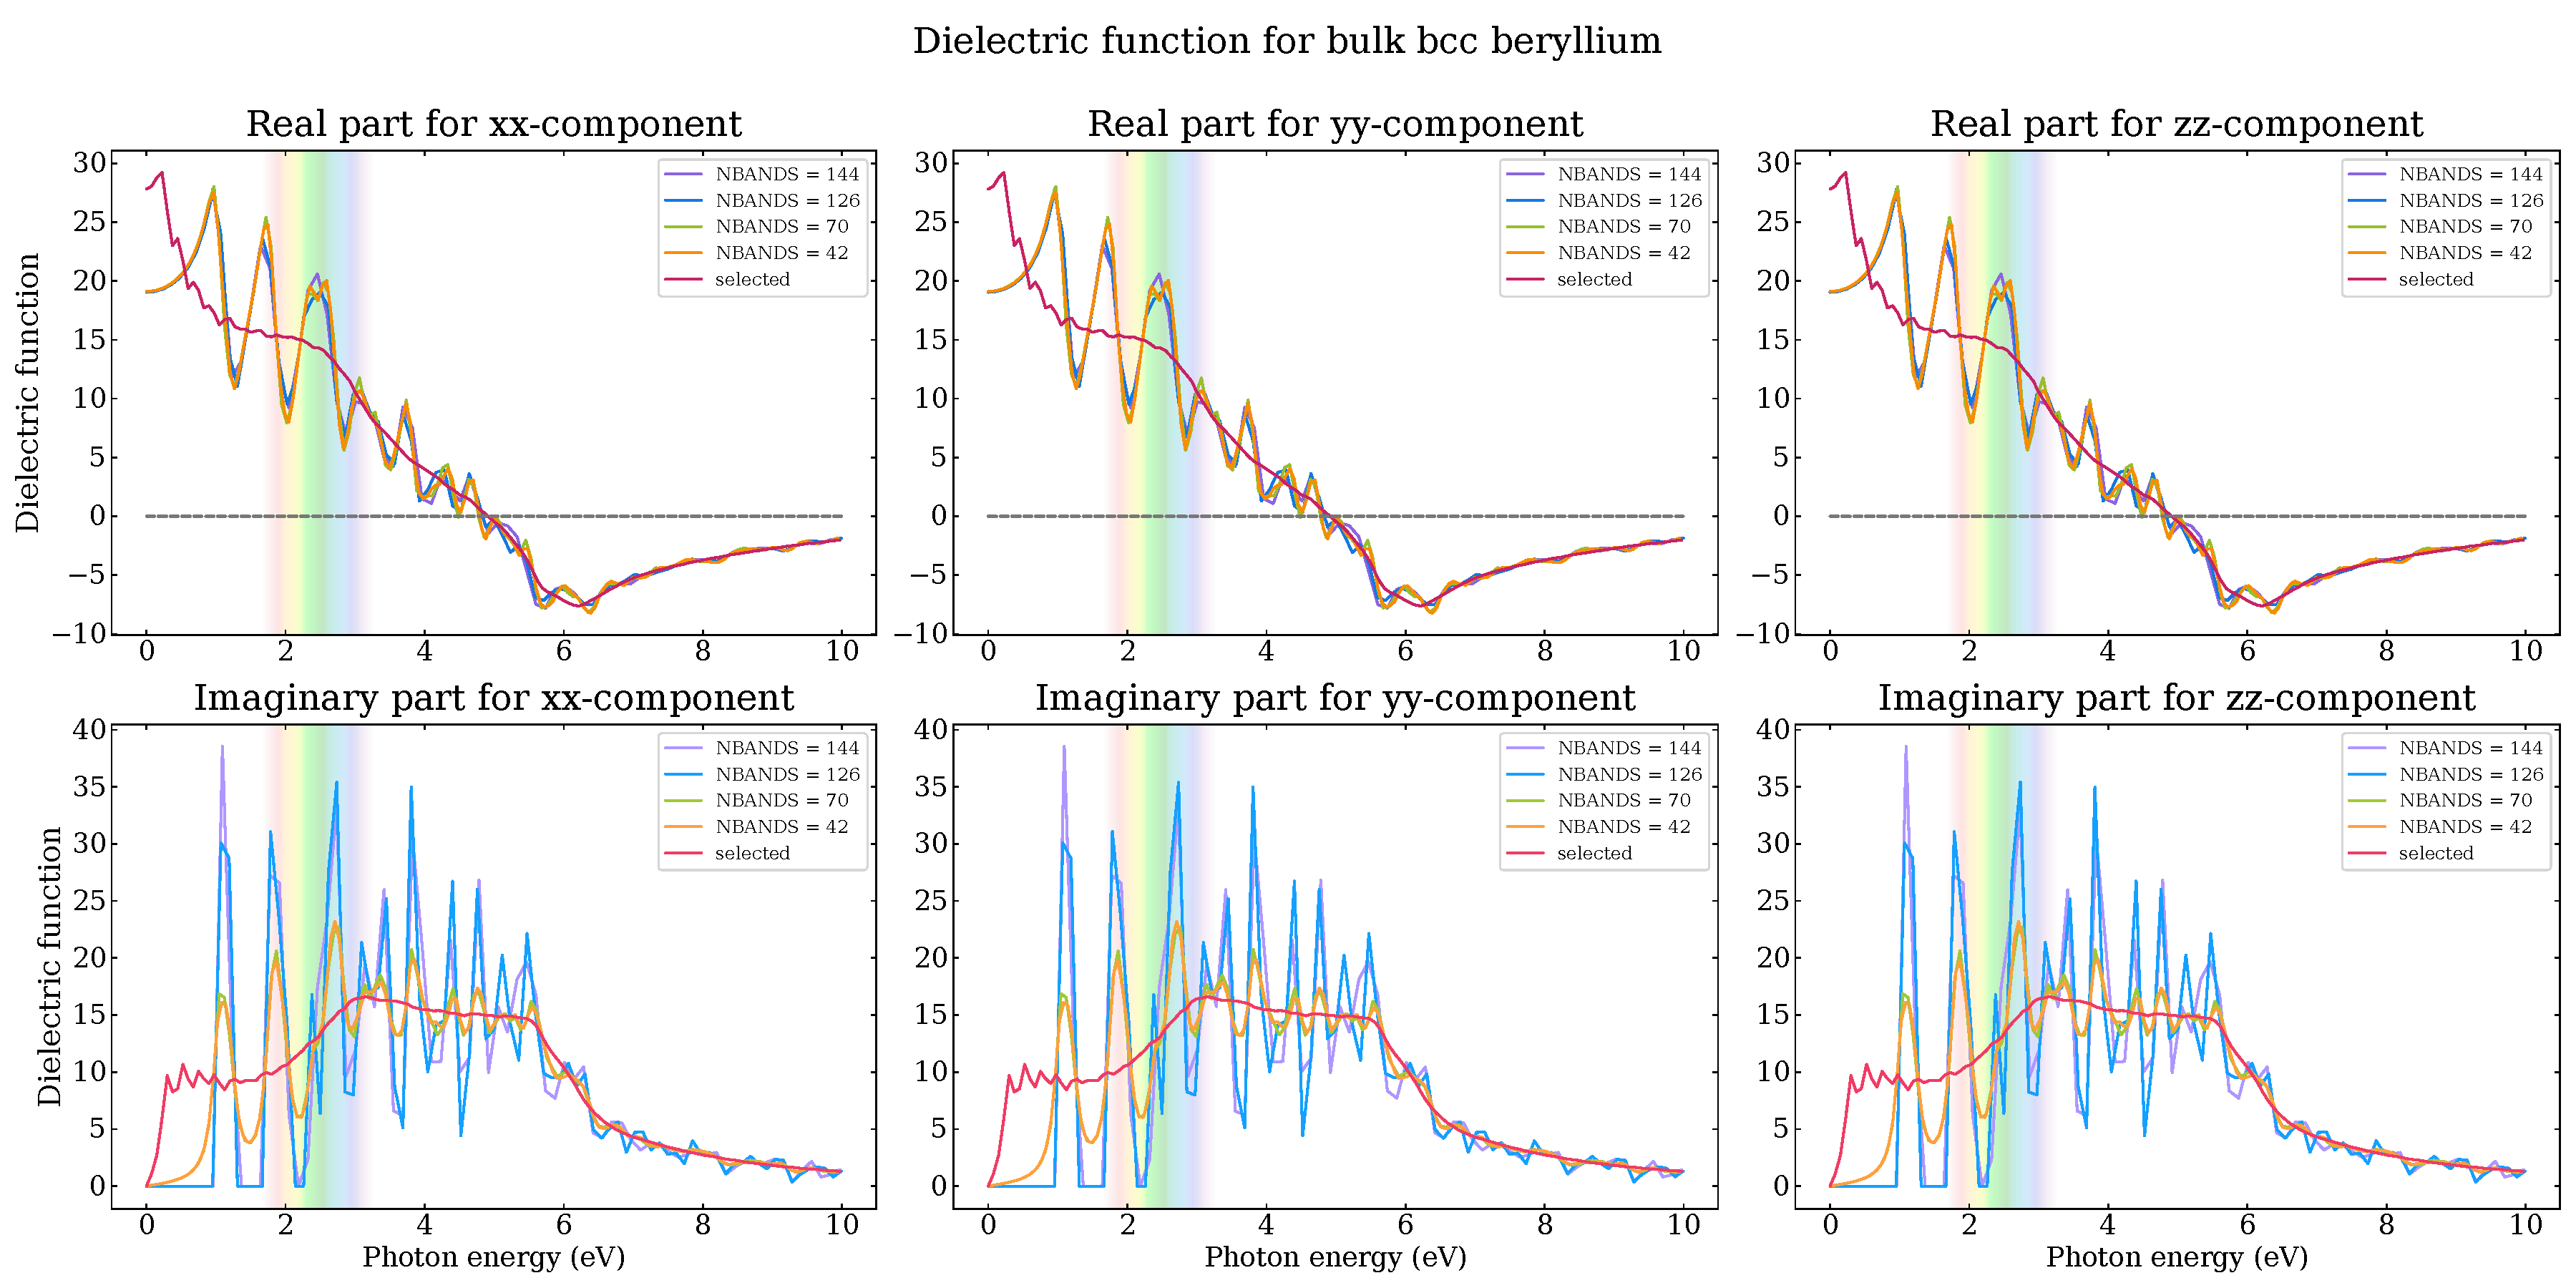
\includegraphics[width=1.0\linewidth]{figures_proj3/convergence_dielectric_nbands_bcc-beryllium_thesis.pdf}
\caption{Real and imaginary parts of the dielectric function for bulk bcc beryllium,
calculated with different total numbers of bands included in the calculation.}
\label{fig:proj3_bcc_dielectric_nbands_convergence}
\end{figure}

\begin{figure}[!htbp]
\centering
    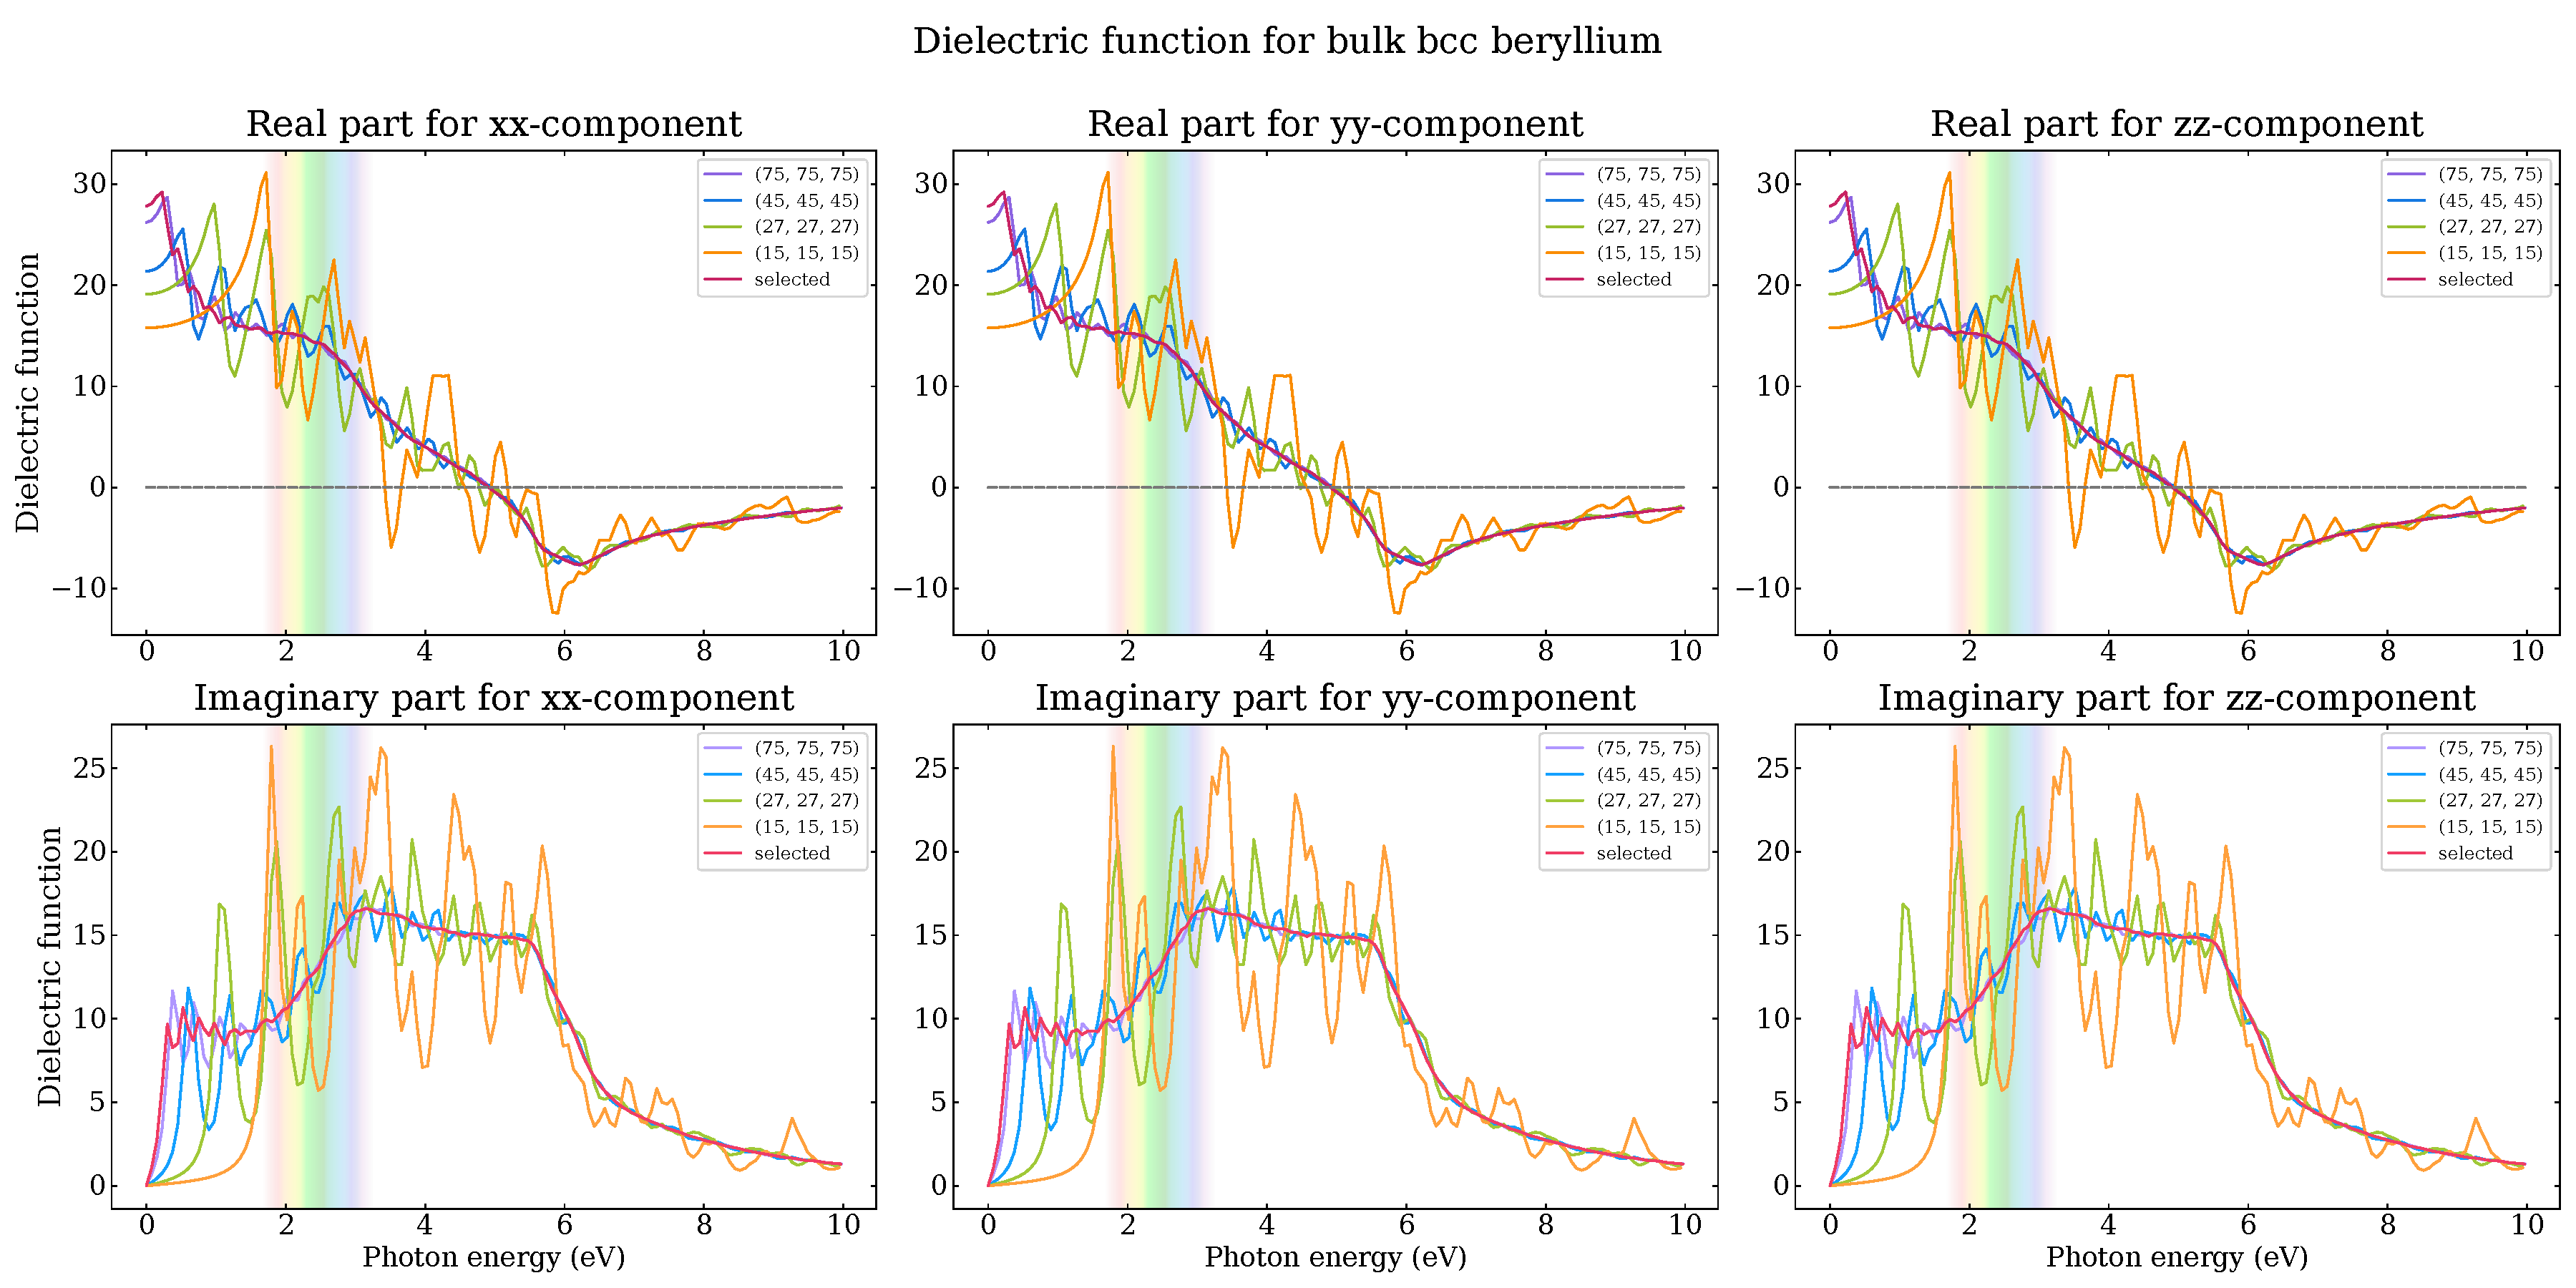
\includegraphics[width=1.0\linewidth]{figures_proj3/convergence_dielectric_kpoints_bcc-beryllium_thesis.pdf}
\caption{Real and imaginary parts of the dielectric function for bulk bcc beryllium,
calculated with different k-point sets.}
\label{fig:proj3_bcc_dielectric_kpoint_convergence}
\end{figure}

\begin{figure}[!htbp]
\centering
    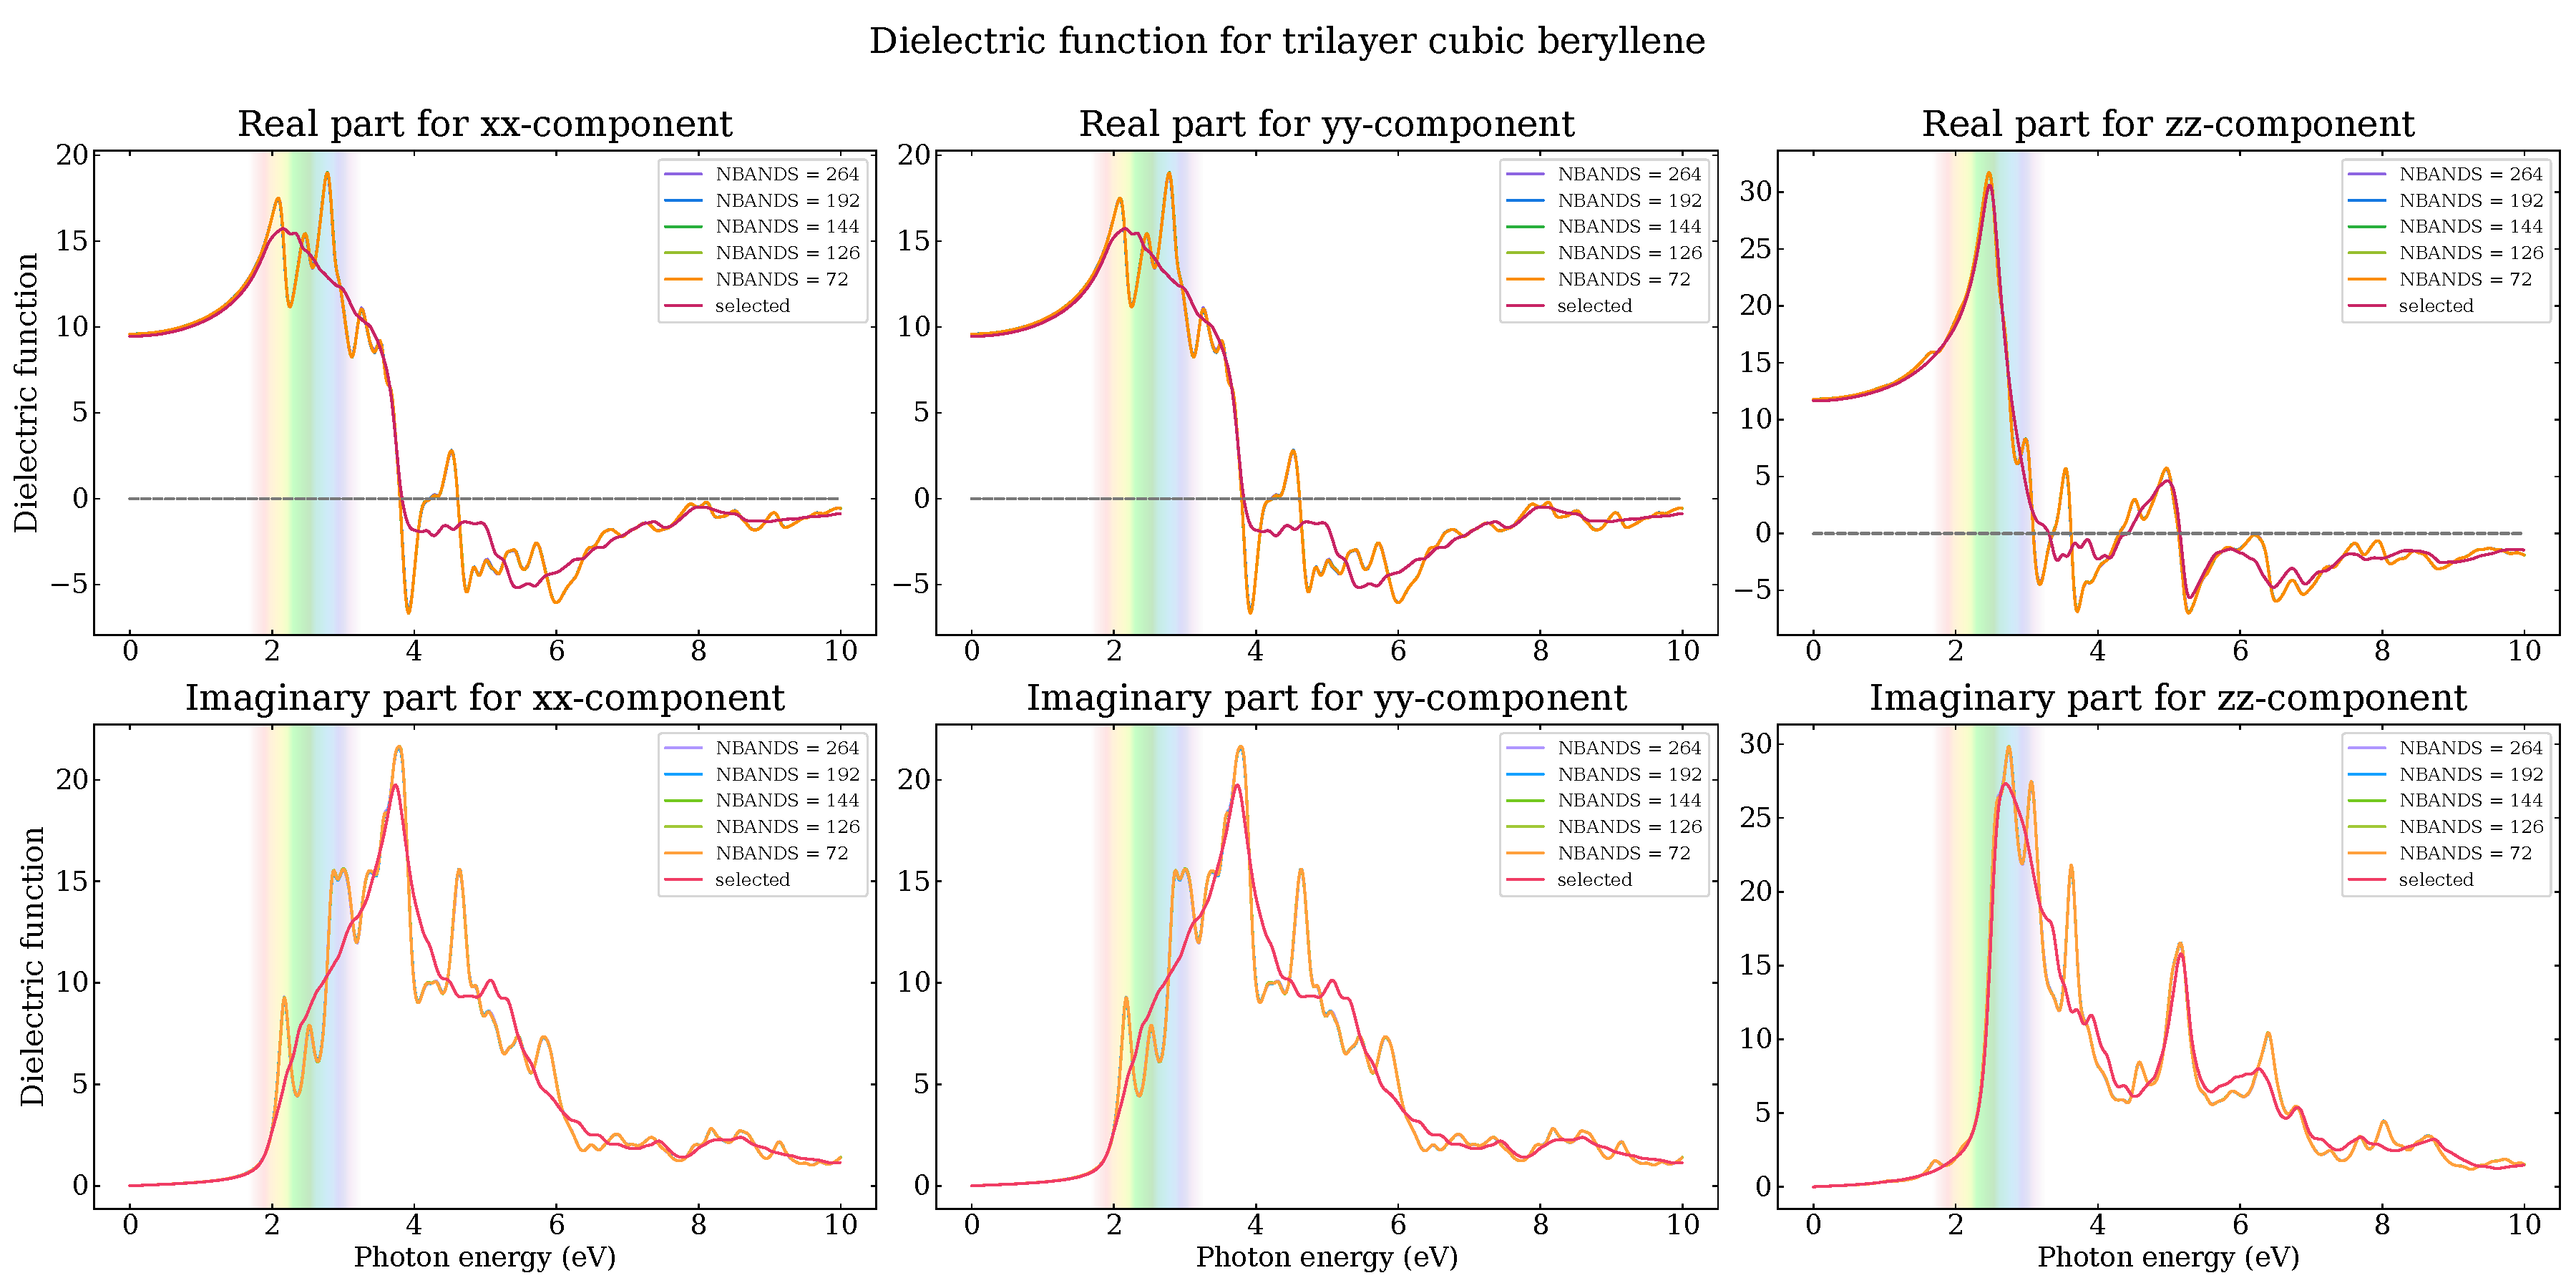
\includegraphics[width=1.0\linewidth]{figures_proj3/convergence_dielectric_nbands_cubic-beryllene-trilayer_thesis.pdf}
\caption{Real and imaginary parts of the dielectric function for trilayer cubic beryllene,
calculated with different total numbers of bands included in the calculation.}
\label{fig:proj3_cubic_dielectric_nbands_convergence}
\end{figure}

\begin{figure}[!htbp]
\centering
    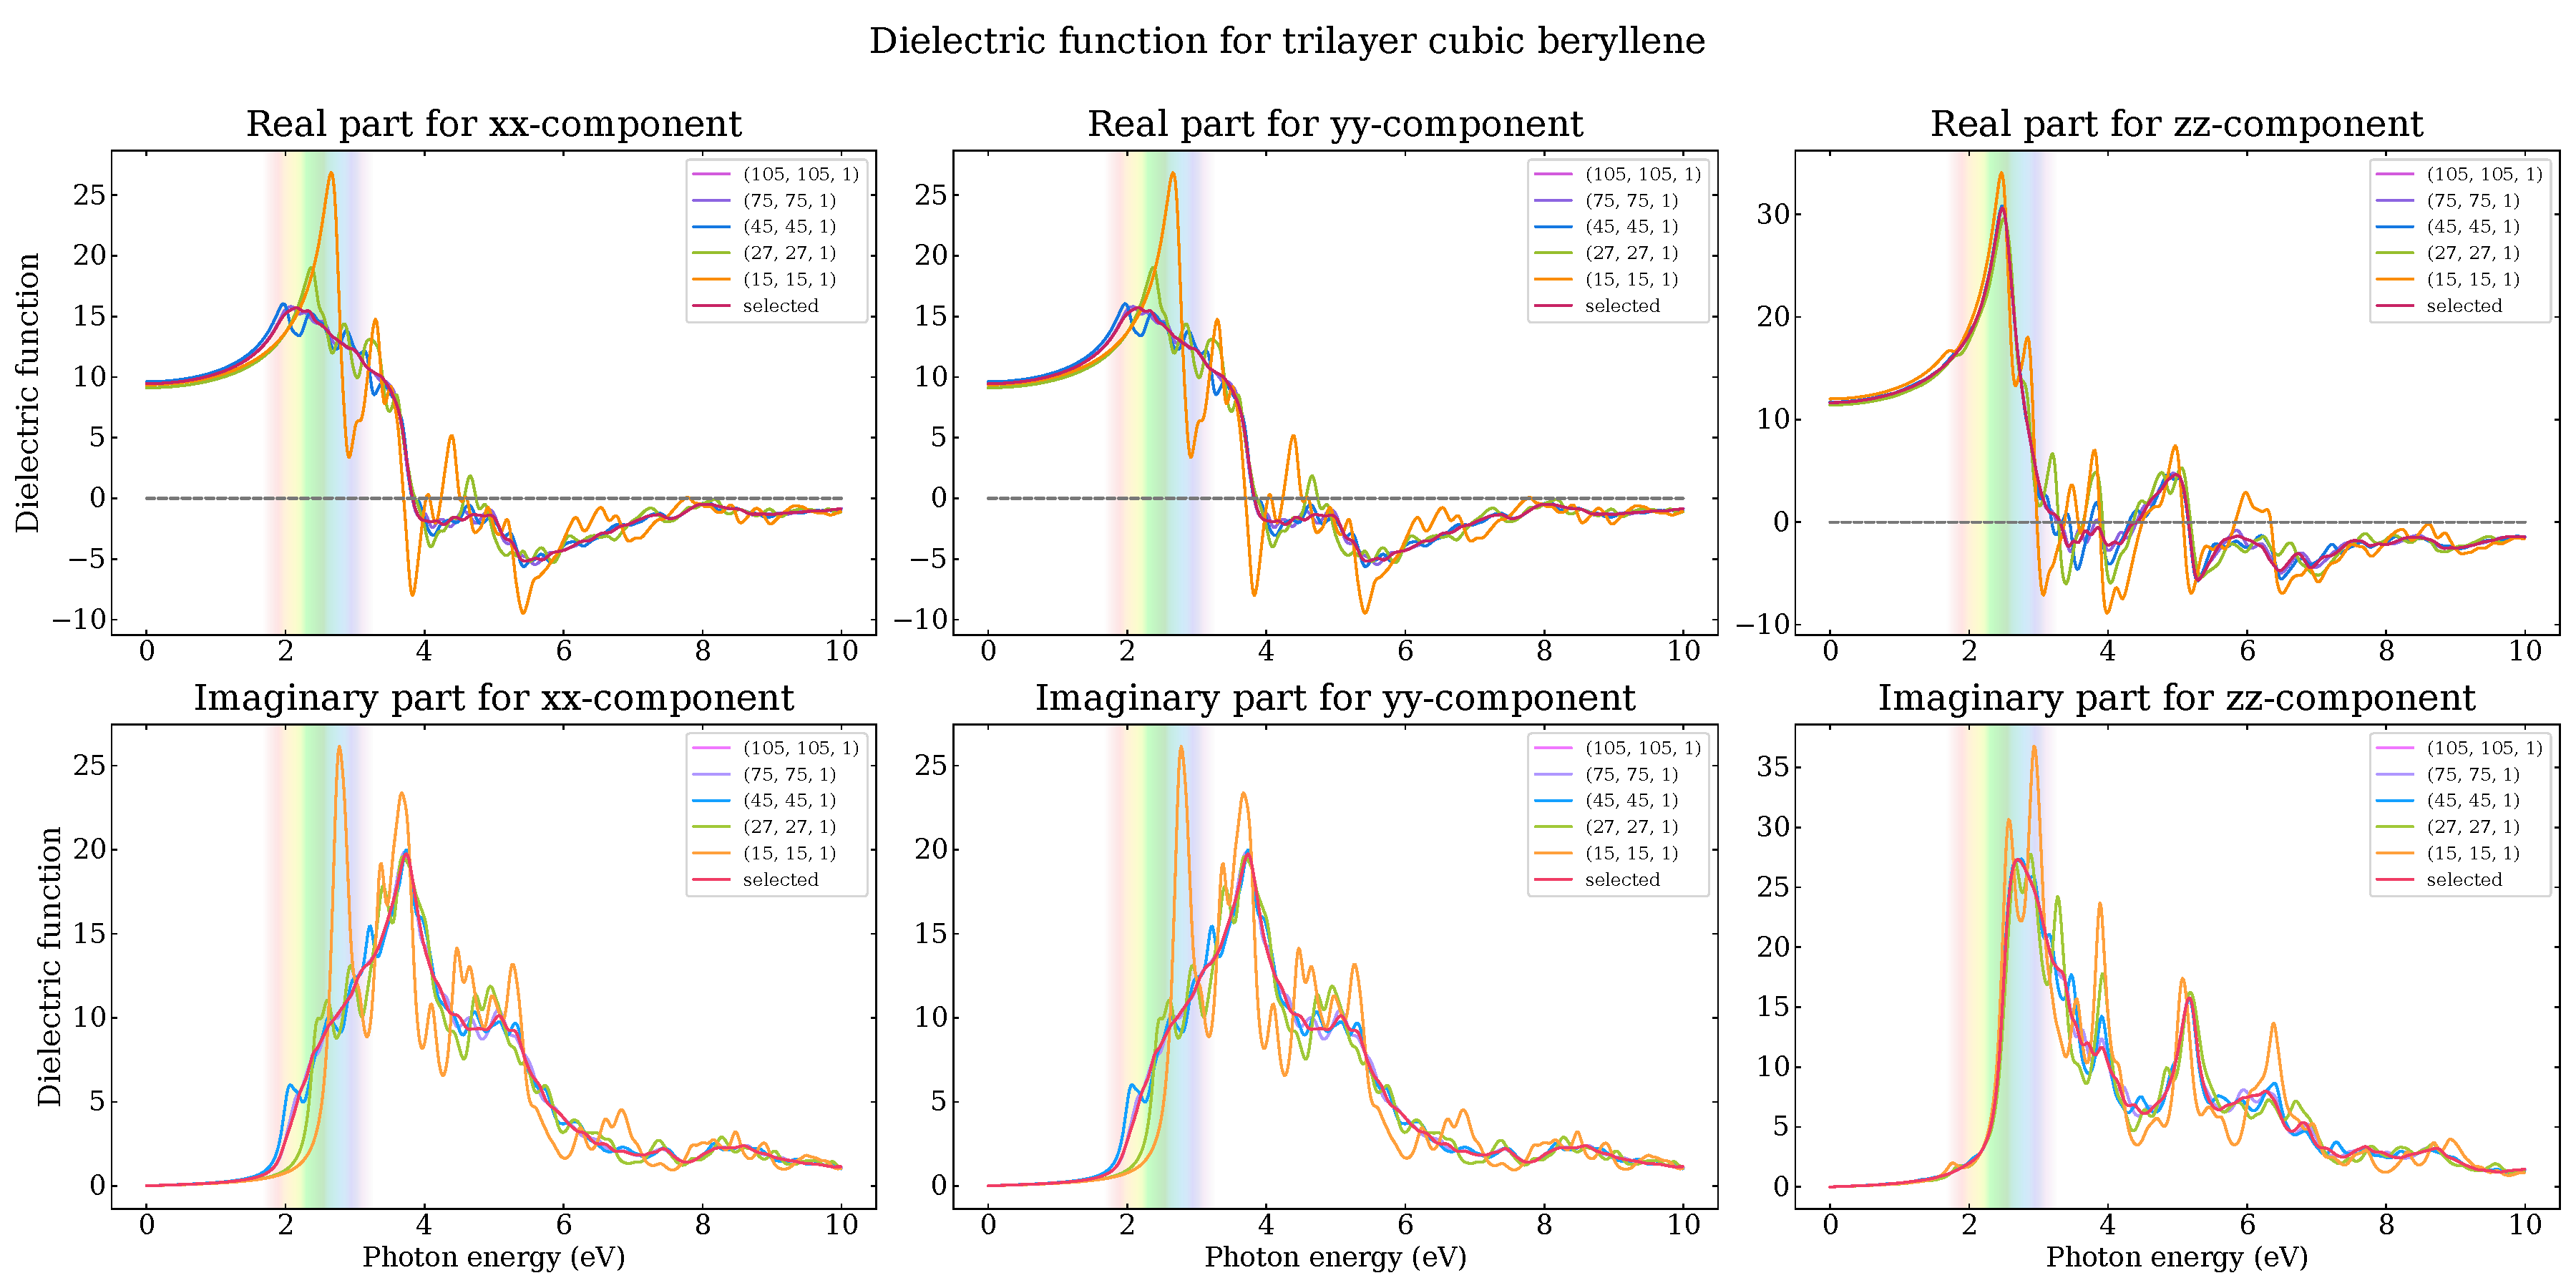
\includegraphics[width=1.0\linewidth]{figures_proj3/convergence_dielectric_kpoints_cubic-beryllene-trilayer_thesis.pdf}
\caption{Real and imaginary parts of the dielectric function for trilayer cubic beryllene,
calculated with different k-point sets.}
\label{fig:proj3_cubic_dielectric_kpoint_convergence}
\end{figure}

\subsection*{Phonon dispersions, Brillouin zones, and band structures}

The calculated phonon dispersion curves and band structures for $\alpha$-beryllene,
$\beta$-beryllene, bulk hcp beryllium, and bulk bcc beryllium
are shown in figures~\ref{fig:proj3_phonon_dispersion} and~\ref{fig:proj3_band_structures}.
The phonon dispersions are calculated with PBE without a dispersion correction.
Bulk bcc beryllium has an imaginary frequency of $3.90i$~\si{\tera\hertz} at the $\mathrm{N}$ point,
which is commensurate with the $4 \times 4 \times 4$ supercell.
This is expected for the high-temperature bcc phase of beryllium,
which is stabilized by anharmonicity.
The Brillouin zones used for the hexagonal and distorted hexagonal cells are shown in figure~\ref{fig:proj3_brillouin_zones}.
For 1H-$\beta$-beryllene and 2H-$\beta$-beryllene,
the band structures and phonon dispersions use the path $\Gamma$--$\mathrm{X}$--$\mathrm{K}$--$\Gamma$--$\mathrm{Y}$--$\mathrm{K}'$--$\mathrm{M}$--$\Gamma$ shown in figure~\ref{fig:proj3_brillouin_zones}(b).
These cells are continuous distortions of the hexagonal cell,
with angles of \qty{117}{\degree} and \qty{133}{\degree} between the lattice vectors,
so $\mathrm{K}$ and $\mathrm{K}'$ derive from the zone corners of the hexagonal cell,
and $\mathrm{X}$, $\mathrm{Y}$, and $\mathrm{M}$ from its three equivalent $\mathrm{M}$ points.
With the $P1$ and $P\bar{1}$ symmetry of 1H-$\beta$-beryllene and 2H-$\beta$-beryllene,
together with time-reversal symmetry,
this path covers the irreducible part of the zone boundary.
Within a tolerance of \qty{1e-3}{\angstrom},
the two cells have $Cm$ and $C2/m$ symmetry,
which makes the $\Gamma$--$\mathrm{Y}$ and $\Gamma$--$\mathrm{M}$ lines of 1H-$\beta$-beryllene and the $\Gamma$--$\mathrm{X}$ and $\Gamma$--$\mathrm{Y}$ lines of 2H-$\beta$-beryllene equivalent;
the calculated PBE bands along these lines differ by at most \qty{3.3}{\milli\electronvolt} and \qty{7.3}{\milli\electronvolt},
respectively.

\begin{figure}[!htbp]
\centering
\begin{tabular}{@{}cc@{}}
% \begin{tabular}{cc}
    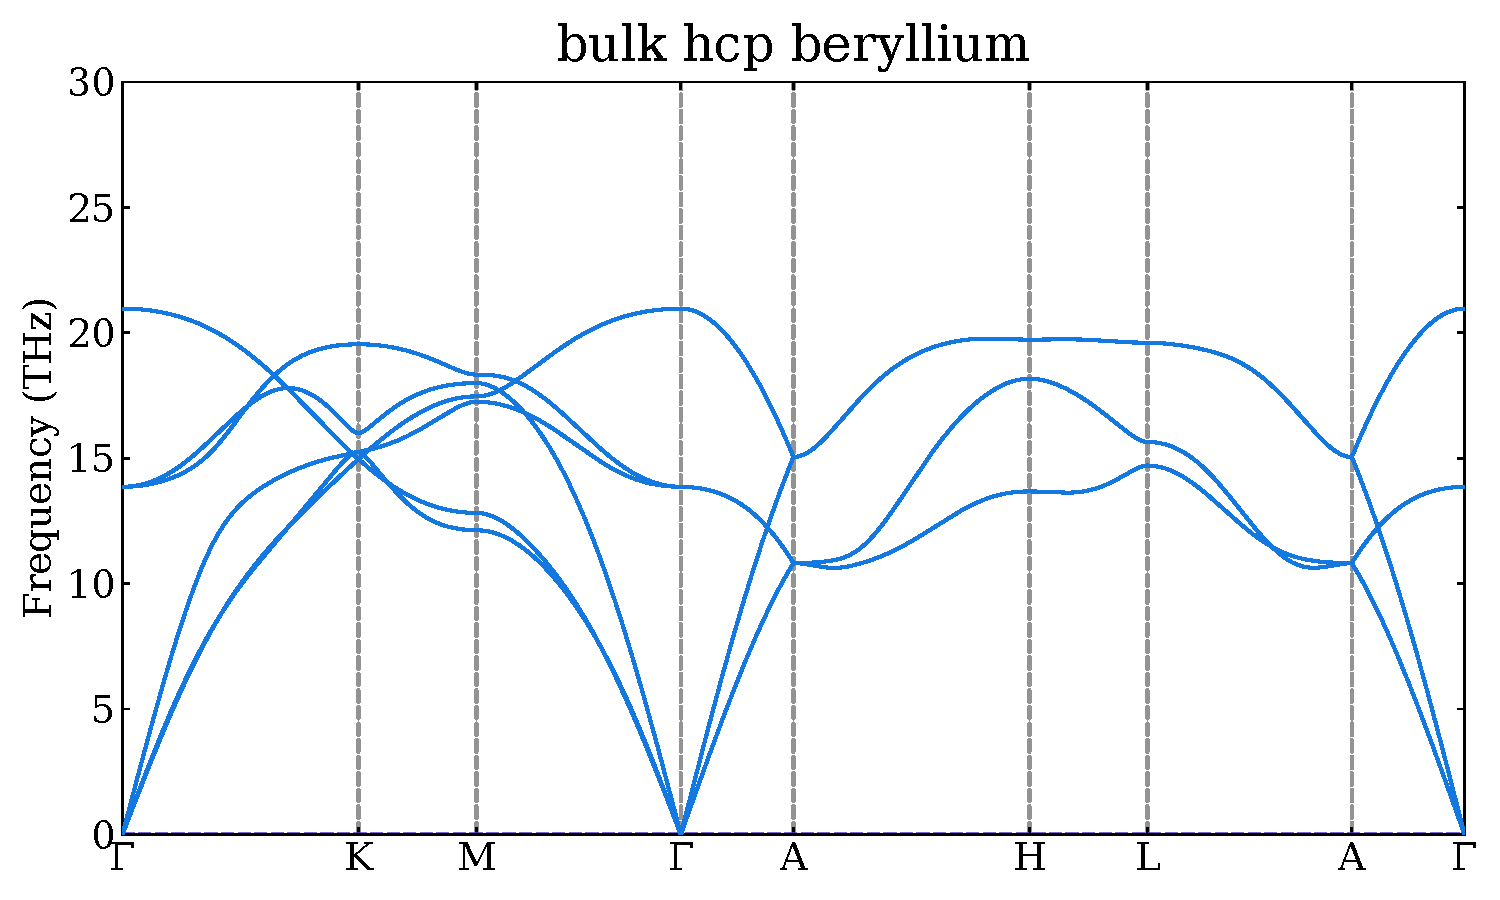
\includegraphics[width=0.40\linewidth]{figures_proj3/phonon_hcp-beryllium_thesis.pdf}&
    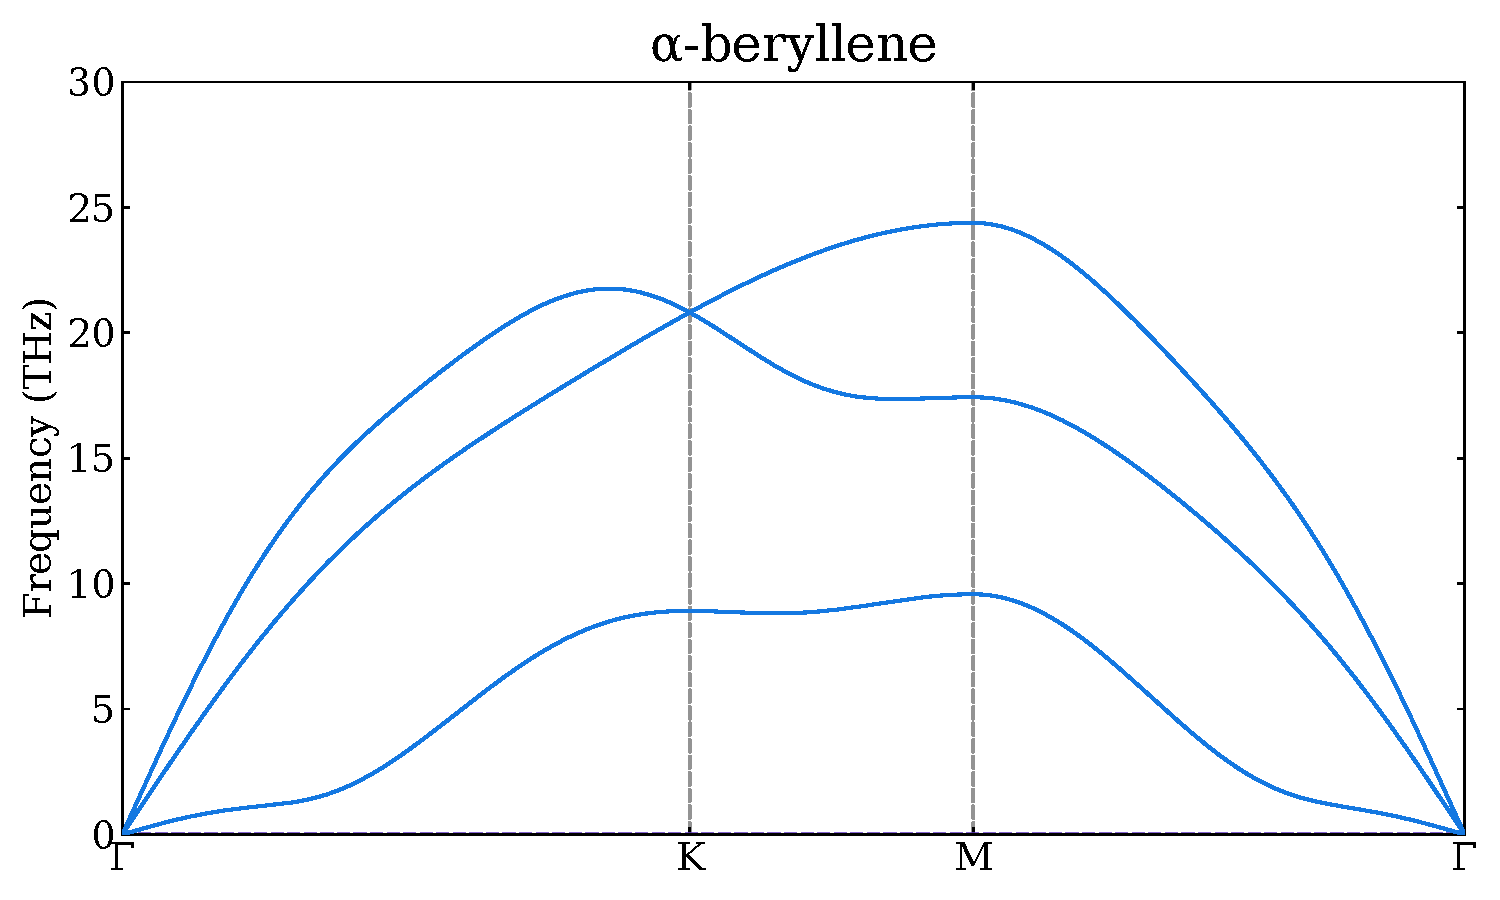
\includegraphics[width=0.40\linewidth]{figures_proj3/phonon_alpha-beryllene_thesis.pdf}\\
    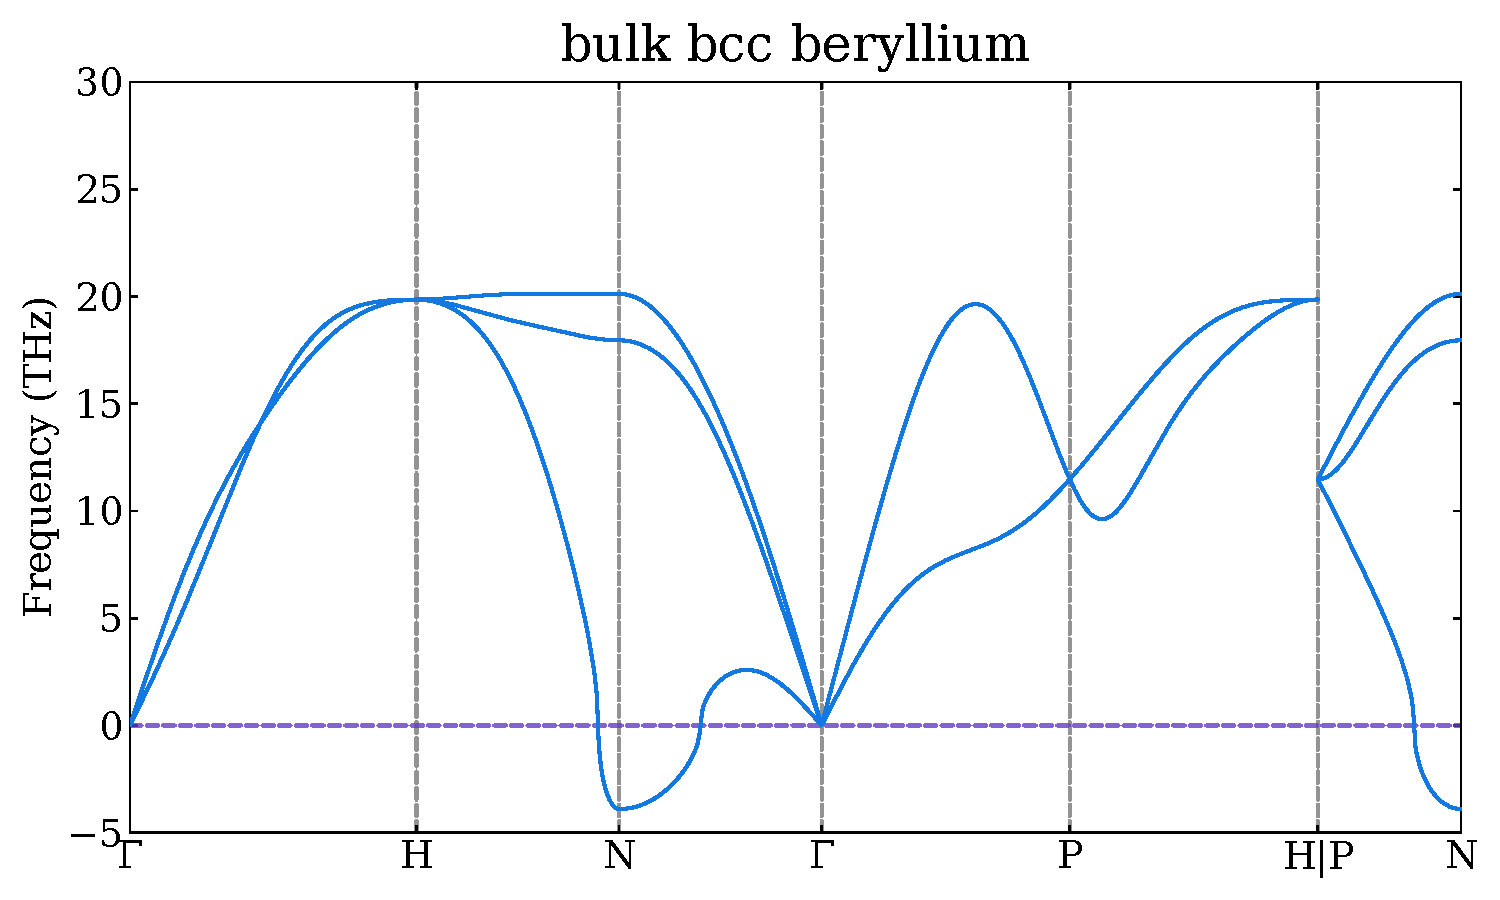
\includegraphics[width=0.40\linewidth]{figures_proj3/phonon_bcc-beryllium_thesis.pdf}&
    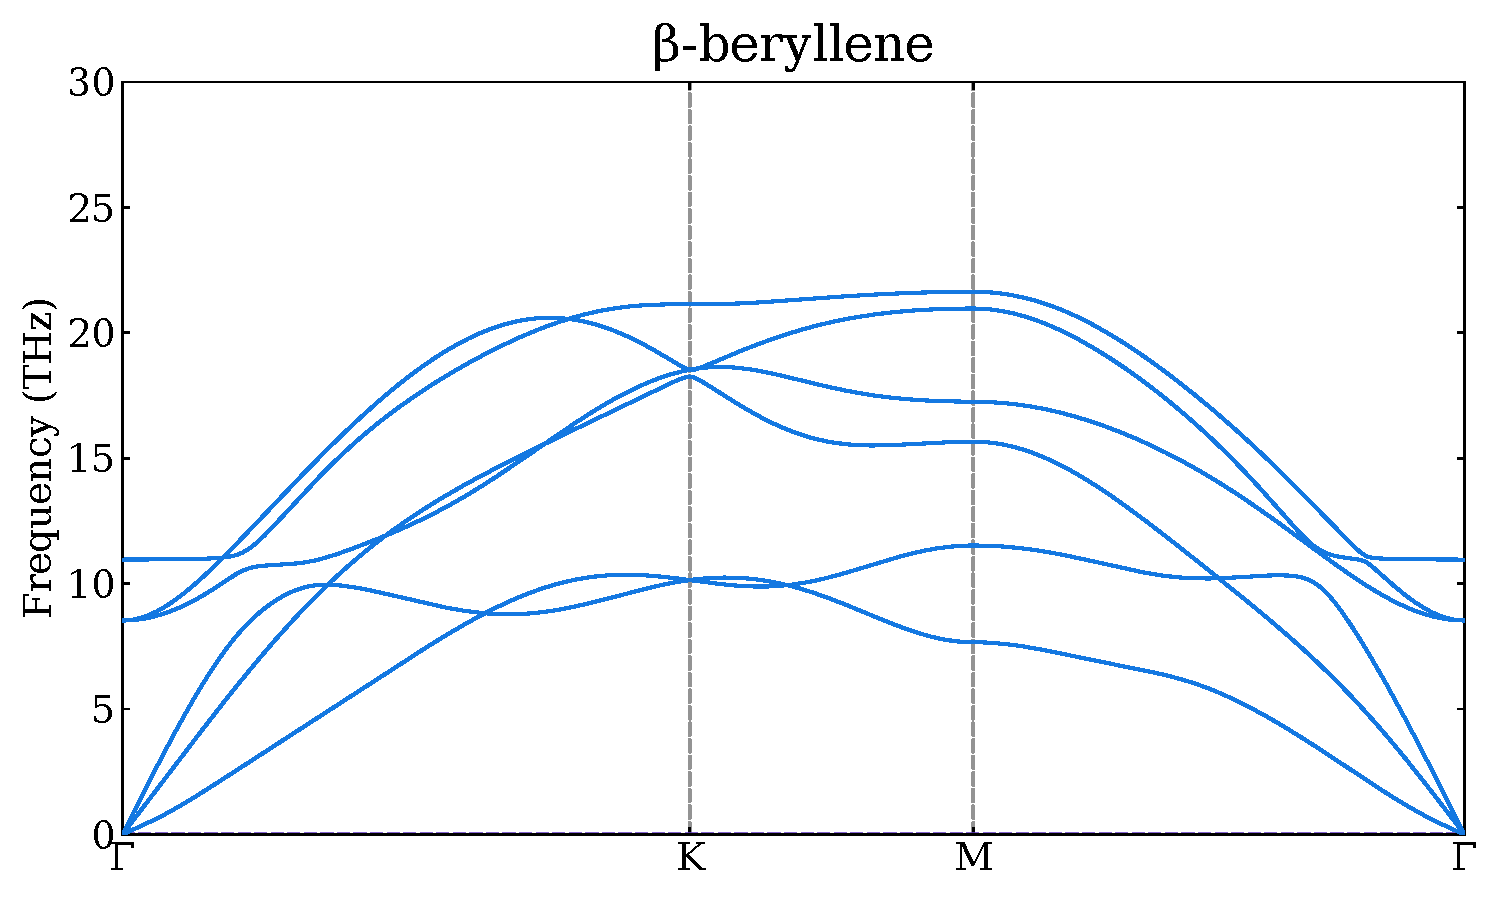
\includegraphics[width=0.40\linewidth]{figures_proj3/phonon_beta-beryllene_thesis.pdf}
\end{tabular}
\caption{Phonon dispersion curves for bulk hcp beryllium, $\alpha$-beryllene, bulk bcc beryllium, and $\beta$-beryllene.
Imaginary frequencies are shown as negative values.}
\label{fig:proj3_phonon_dispersion}
\end{figure}

\begin{figure}[!htbp]
\centering
    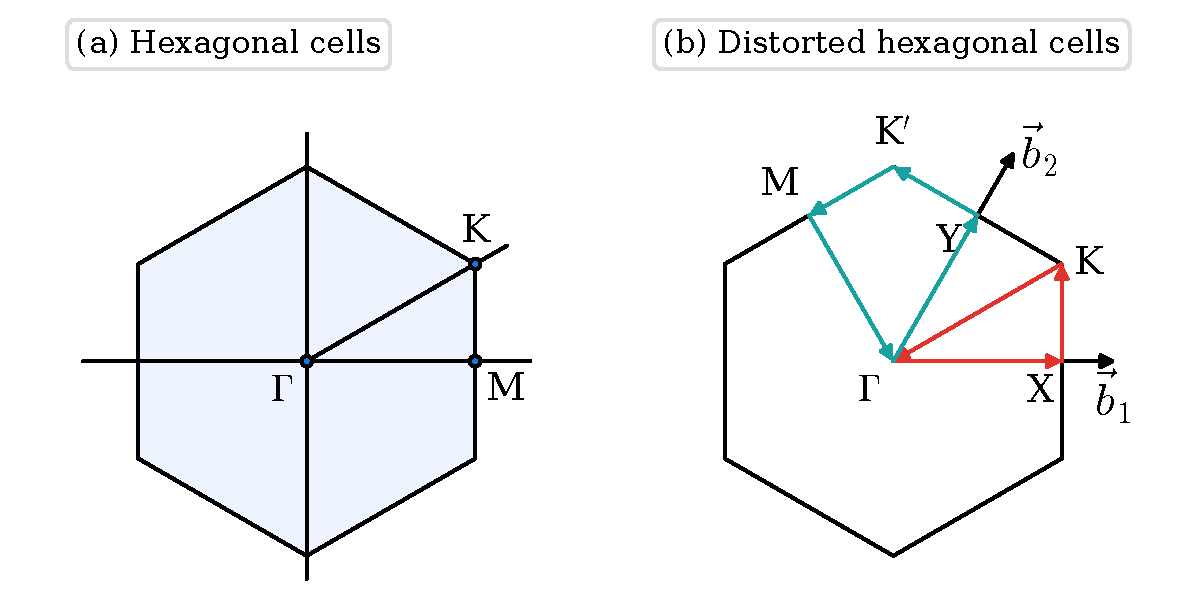
\includegraphics[width=0.80\linewidth]{figures_proj3/brillouin_zone_thesis.pdf}
\caption{Schematic Brillouin zones of the hexagonal and distorted hexagonal cells.
(a) Brillouin zone for the hexagonal unit cells of $\alpha$-beryllene, $\beta$-beryllene, and 2H-$\alpha$-beryllene;
(b) Brillouin zone for the distorted hexagonal cells of 1H-$\beta$-beryllene and 2H-$\beta$-beryllene,
with the path $\Gamma$--$\mathrm{X}$--$\mathrm{K}$--$\Gamma$--$\mathrm{Y}$--$\mathrm{K}'$--$\mathrm{M}$--$\Gamma$ used for their band structures and phonon dispersions.
$\vec{b}_{1}$ and $\vec{b}_{2}$ are the reciprocal lattice vectors of each relaxed cell,
and all coordinates are given in this basis.
$\mathrm{X}=\vec{b}_{1}/2$,
$\mathrm{Y}=\vec{b}_{2}/2$,
and $\mathrm{M}=(\vec{b}_{2}-\vec{b}_{1})/2$,
which is equivalent to $(\vec{b}_{1}+\vec{b}_{2})/2$,
are the time-reversal invariant momenta on the zone boundary.
$\mathrm{K}$ and $\mathrm{K}'=-\mathrm{K}+\vec{b}_{2}$ are the zone corners,
which are related by time reversal,
with $\mathrm{K}=(0.315,\,0.370)$ for 1H-$\beta$-beryllene and $(0.298,\,0.298)$ for 2H-$\beta$-beryllene.}
\label{fig:proj3_brillouin_zones}
\end{figure}

\begin{figure}[!htbp]
\centering
\begin{tabular}{@{}cc@{}}
% \begin{tabular}{cc}
    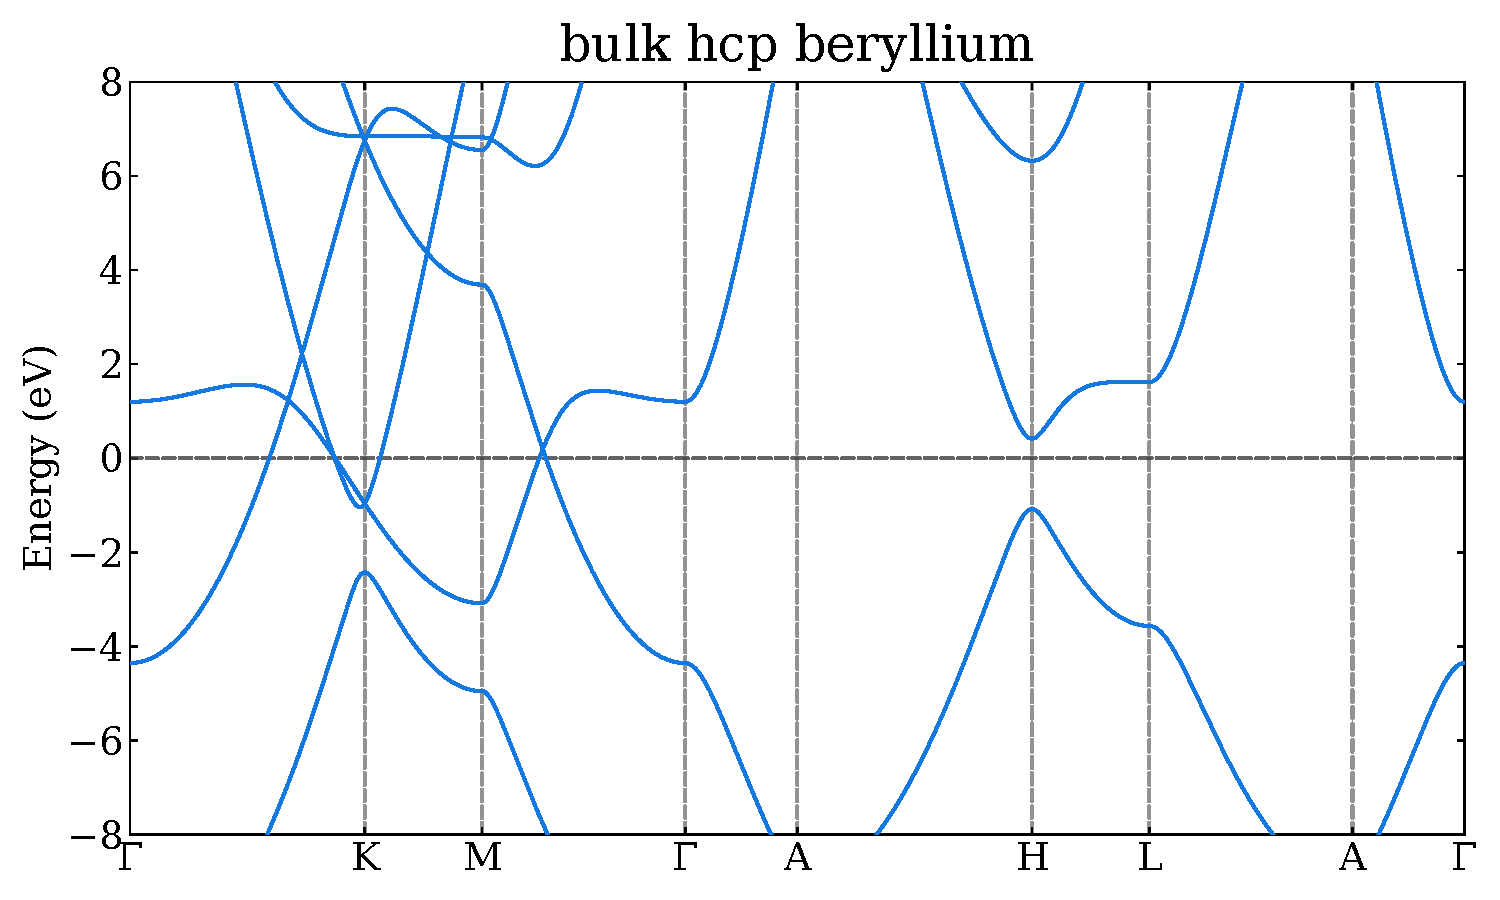
\includegraphics[width=0.40\linewidth]{figures_proj3/bands_hcp-beryllium_thesis.pdf}&
    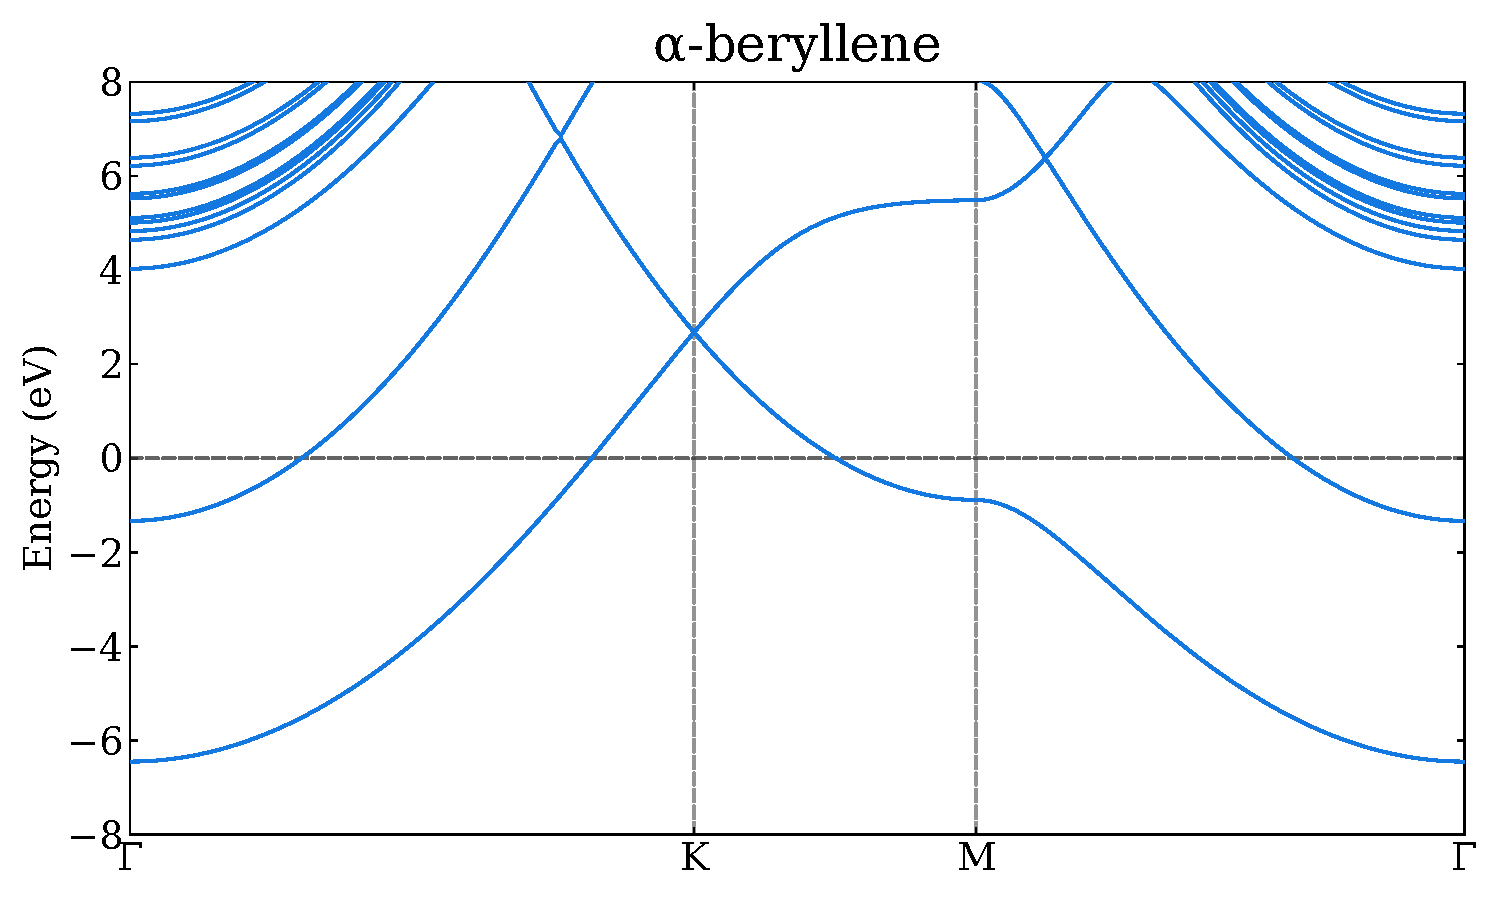
\includegraphics[width=0.40\linewidth]{figures_proj3/bands_alpha-beryllene_thesis.pdf}\\
    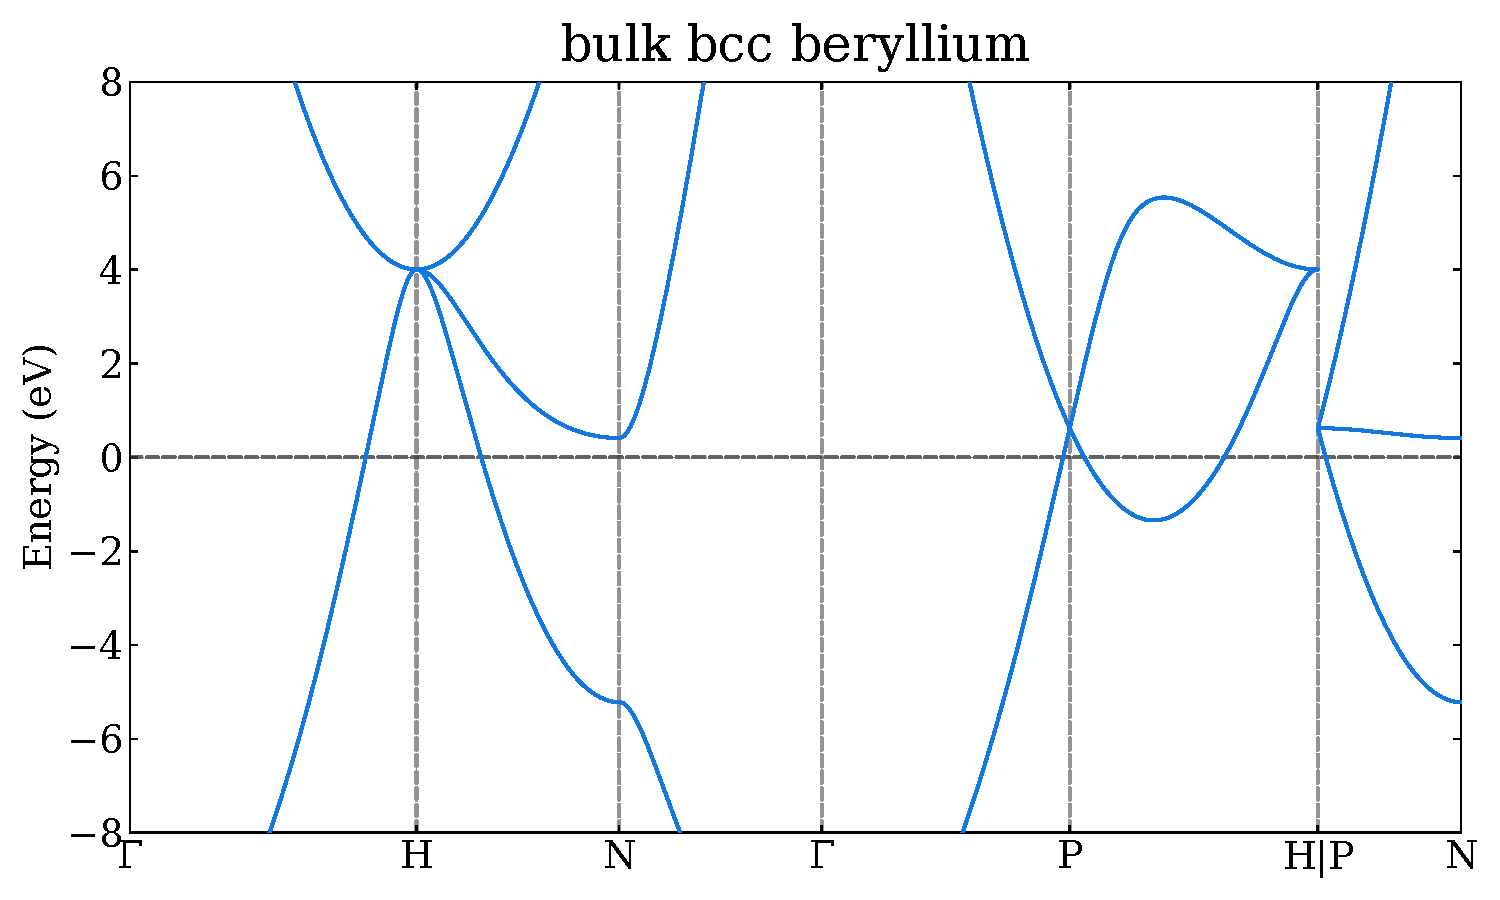
\includegraphics[width=0.40\linewidth]{figures_proj3/bands_bcc-beryllium_thesis.pdf}&
    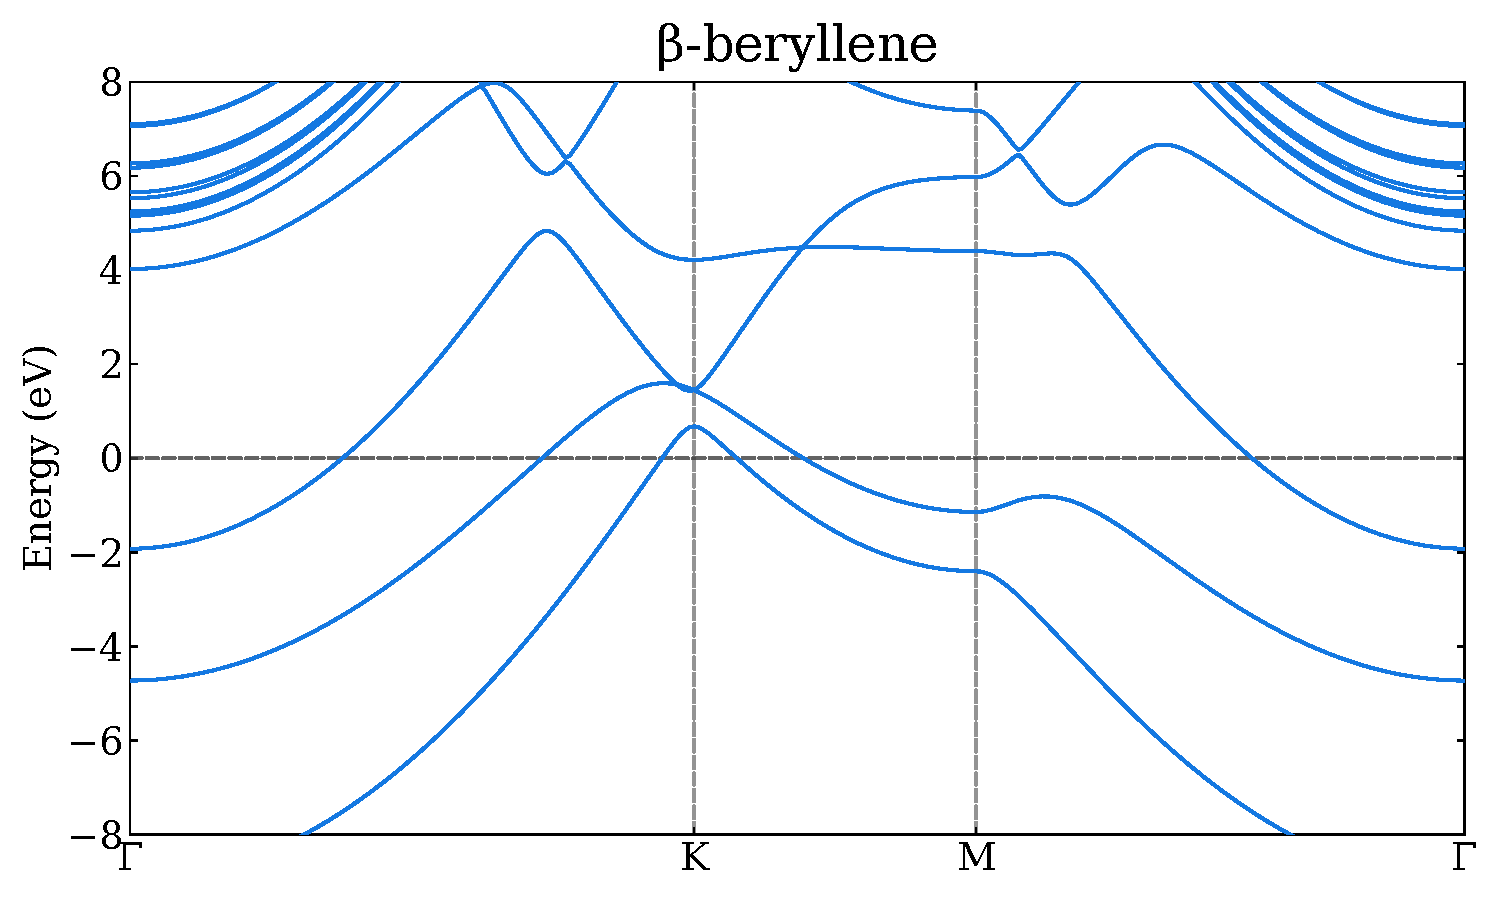
\includegraphics[width=0.40\linewidth]{figures_proj3/bands_beta-beryllene_thesis.pdf}
\end{tabular}
\caption{Band structures of bulk hcp beryllium, $\alpha$-beryllene, bulk bcc beryllium, and $\beta$-beryllene.}
\label{fig:proj3_band_structures}
\end{figure}

\subsection*{Soft mode of 2H-$\beta$-beryllene}

The soft mode of 2H-$\beta$-beryllene lies at the wave vector $\vec{q}=(-0.4,0.4)$ on the $\Gamma$--$\mathrm{M}$ line,
in units of the reciprocal lattice vectors,
which is commensurate with the $5 \times 5$ phonon supercell.
For the frozen-phonon calculations,
we use a 20-atom supercell with lattice vectors $\vec{A}_{1}=5\vec{a}_{1}$ and $\vec{A}_{2}=\vec{a}_{1}+\vec{a}_{2}$,
which is also commensurate with this wave vector.
The atoms are displaced along the eigenvector of the soft mode,
with maximum displacements of \qty{0.025}{\angstrom}, \qty{0.049}{\angstrom}, and \qty{0.098}{\angstrom},
and the total energy is calculated at each amplitude without further relaxation.
These calculations are repeated with Gaussian smearing of \qty{0.02}{\electronvolt}, \qty{0.05}{\electronvolt}, and \qty{0.10}{\electronvolt},
using k-point meshes of $16 \times 97 \times 1$ for \qty{0.02}{\electronvolt} and $11 \times 65 \times 1$ otherwise.
The energies are fitted to $E(Q)-E(0)=aQ^{2}+bQ^{4}$,
where $Q$ is the mass-weighted amplitude of the mode.
The curvature $a$ gives the harmonic frequency,
and $a^{2}/4b$ gives the depth of the double well for $a<0$.
The fitted harmonic frequencies of $1.0i$--$1.8i$~\si{\tera\hertz} are comparable with the value of $1.65i$~\si{\tera\hertz} from the phonon calculation.

To estimate the effect of quantum fluctuations,
we solve the one-dimensional Schr\"odinger equation for the fitted potential numerically,
and also calculate the self-consistent harmonic frequency $\Omega$ of this single mode,
which satisfies $\Omega^{2}=2a+12b\langle Q^{2}\rangle$,
with $\langle Q^{2}\rangle=(\hbar/2\Omega)\coth(\hbar\Omega/2k_{\mathrm{B}}T)$.
The coupling to the other phonon modes is neglected,
so these values indicate the size of the quantum fluctuations rather than replacing a full anharmonic phonon calculation.
The results are listed in table~\ref{tab:proj3_soft_mode}.
For all three smearing values,
the ground state lies approximately \qty{6}{\milli\electronvolt} above the bottom of the double well,
far above the well depth,
and the first excitation energy corresponds to approximately \qty{4}{\tera\hertz}.
The root-mean-square amplitude of the ground state,
0.35--0.36~amu$^{1/2}$\,\AA,
exceeds the position of the potential minimum,
0.14--0.24~amu$^{1/2}$\,\AA.
For a smearing of \qty{0.02}{\electronvolt},
the maximum fit residual of \qty{0.16}{\milli\electronvolt} is comparable to the fitted well depth,
so this depth is only an upper estimate.

\begin{table}[!htbp]
\centering
\rowcolors{2}{gray!15}{white}
\begin{adjustbox}{center,max width=1.0\linewidth}
\begin{tabular}{lccc}
\hline
\rowcolor{gray!25}
Gaussian smearing (eV) & 0.02 & 0.05 & 0.10 \\
supercell k-point mesh & $16 \times 97 \times 1$ & $11 \times 65 \times 1$ & $11 \times 65 \times 1$ \\
\hline
$\Delta E$ at \qty{0.025}{\angstrom} (meV) & $0.015$ & $-0.013$ & $-0.012$ \\
$\Delta E$ at \qty{0.049}{\angstrom} (meV) & $-0.007$ & $0.578$ & $0.495$ \\
$\Delta E$ at \qty{0.098}{\angstrom} (meV) & $10.029$ & $12.450$ & $11.932$ \\
fitted harmonic frequency (THz) & $1.75i$ & $1.02i$ & $1.13i$ \\
double-well depth (meV) & $0.185$ & $0.021$ & $0.032$ \\
maximum fit residual (meV) & $0.158$ & $0.001$ & $0.018$ \\
\hline
ground state above the well bottom (meV) & $5.88$ & $6.31$ & $6.21$ \\
first excitation energy (THz) & $3.77$ & $4.00$ & $3.95$ \\
self-consistent frequency at \qty{0}{\kelvin} (THz) & $4.03$ & $4.23$ & $4.18$ \\
self-consistent frequency at \qty{300}{\kelvin} (THz) & $5.54$ & $5.67$ & $5.63$ \\
\hline
\end{tabular}
\end{adjustbox}
\caption{Frozen-phonon energies $\Delta E$ of the soft mode of 2H-$\beta$-beryllene relative to the undistorted structure,
per 20-atom supercell and at the given maximum atomic displacements,
parameters of the quartic fit,
and the one-mode quantum estimates.}
\label{tab:proj3_soft_mode}
\end{table}

The bare static susceptibility and the nesting function of 2H-$\beta$-beryllene are shown in figure~\ref{fig:proj3_nesting}.
Neither quantity has a peak at the soft-mode wave vector,
so the softening is not driven by Fermi-surface nesting.

\begin{figure}[!htbp]
\centering
    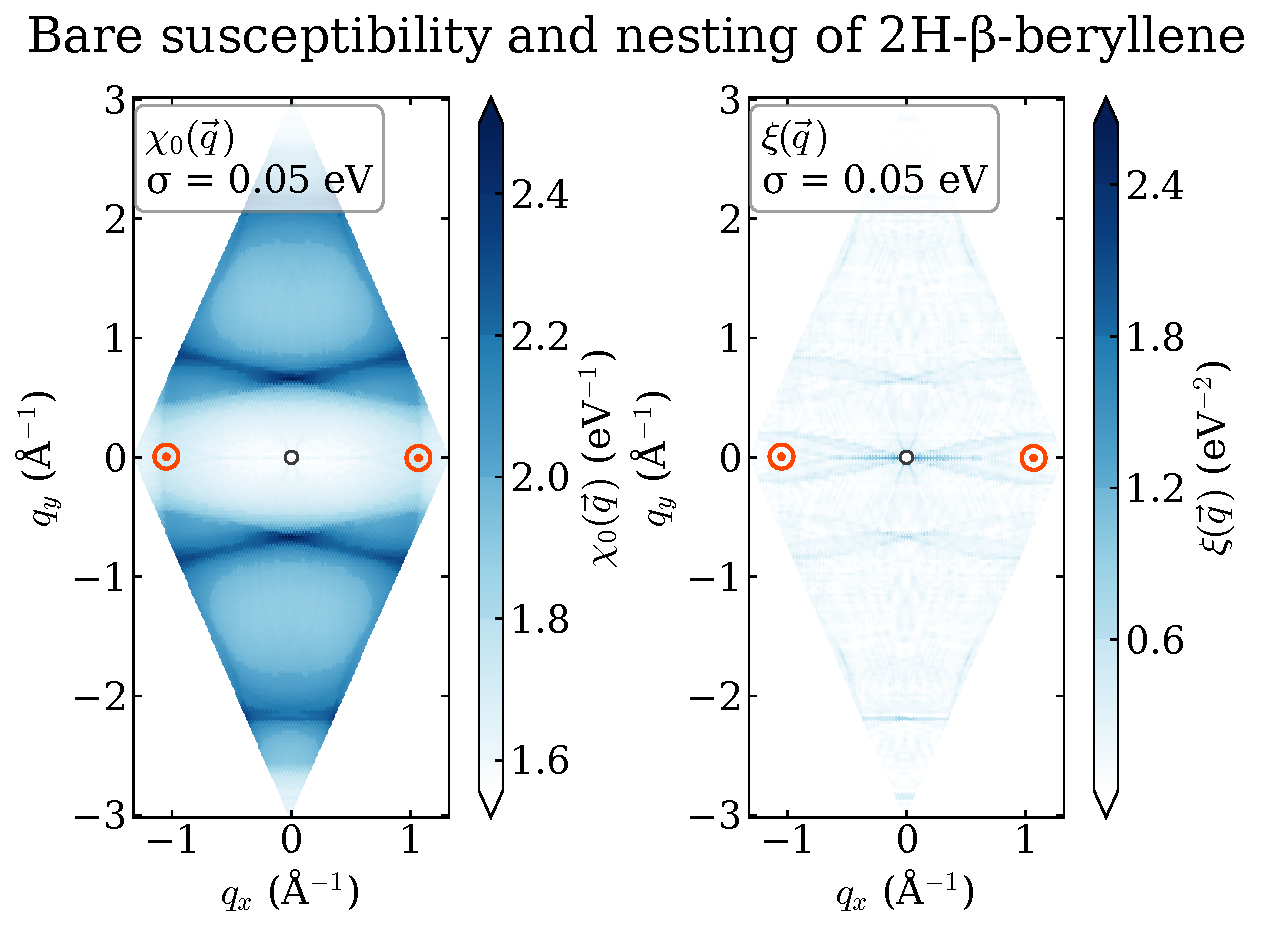
\includegraphics[width=0.80\linewidth]{figures_proj3/nesting_2H-beta-beryllene_thesis.pdf}
\caption{Bare static susceptibility $\chi_{0}(\vec{q})$ (left) and nesting function $\xi(\vec{q})$ (right) of 2H-$\beta$-beryllene,
calculated with constant matrix elements from the spin-orbit-coupled eigenvalues on the $105 \times 105$ grid,
with Gaussian smearing of \qty{0.05}{\electronvolt}.
The bands with states within \qty{1}{\electronvolt} of the Fermi level are included.
The open circles mark the soft-mode wave vector and its symmetry images,
and the value at $\vec{q}=0$ is excluded from the colour scale.
Among the 11024 nonzero wave vectors of the grid,
the soft-mode wave vector ranks between 8723 and 8935 in $\chi_{0}$ and between 3806 and 8405 in $\xi$ for smearing between 0.02 and \qty{0.10}{\electronvolt}.}
\label{fig:proj3_nesting}
\end{figure}

\subsection*{Hydrogenation energetics}

The adsorption energies of hydrogen relative to \ce{H2} are listed in table~\ref{tab:proj3_hydrogenation_energetics},
together with the zero-point energy and finite-temperature corrections.
The zero-point energies of the beryllene layers are calculated from the harmonic phonons on a $40 \times 40$ q-point mesh,
and the zero-point energy of \ce{H2} is \qty{0.269}{\electronvolt}.
The free energies at \qty{298.15}{\kelvin} and \qty{1}{\bar} include the harmonic vibrational free energies of the layers
and the enthalpy and entropy of gaseous \ce{H2},
$H(T)-H(0)-TS=\qty{-0.316}{\electronvolt}$ per \ce{H2}.
The equilibrium \ce{H2} pressure is the pressure at which the adsorption free energy vanishes,
$p_{\mathrm{eq}}=p^{\circ}\exp\left(2\Delta G/k_{\mathrm{B}}T\right)$ with $p^{\circ}=\qty{1}{\bar}$.
The zero-point energy raises all adsorption energies by \qtyrange{0.08}{0.09}{\electronvolt} per hydrogen atom,
because the vibrations of the adsorbed hydrogen atoms outweigh the stretching mode of \ce{H2}.
For 2H-$\beta$-beryllene,
the imaginary phonon modes are excluded from the vibrational free energy;
they cover \qty{1.1}{\percent} of the Brillouin zone,
and their contribution is below \qty{0.1}{\milli\electronvolt} per hydrogen atom.

\begin{table}[!htbp]
\centering
\rowcolors{2}{gray!15}{white}
\begin{tabular}{ccccc}
\hline
\rowcolor{gray!25}
structure
& $\Delta E$ (eV)
& $\Delta E+\Delta E_{\mathrm{ZPE}}$ (eV)
& $\Delta G$ (eV)
& $p_{\mathrm{eq}}$ (bar) \\
\hline
2H-$\alpha$-beryllene & $-0.331$ & $-0.243$ & $-0.084$ & $1.4\times10^{-3}$ \\
1H-$\beta$-beryllene & $-0.072$ & $0.012$ & $0.166$ & $4.0\times10^{5}$ \\
2H-$\beta$-beryllene & $-0.173$ & $-0.090$ & $0.058$ & $93$ \\
\hline
\end{tabular}
\caption{Adsorption energy per hydrogen atom relative to \ce{H2},
$\Delta E$,
the same energy including the zero-point energy correction,
$\Delta E+\Delta E_{\mathrm{ZPE}}$,
the adsorption free energy per hydrogen atom at \qty{298.15}{\kelvin} and \qty{1}{\bar},
$\Delta G$,
and the equilibrium \ce{H2} pressure at \qty{298.15}{\kelvin},
$p_{\mathrm{eq}}$.}
\label{tab:proj3_hydrogenation_energetics}
\end{table}

The relaxed energies of the \ce{BeH2} monolayers are listed in table~\ref{tab:proj3_beh2_polymorphs}.
All four structures are relaxed with the same settings as 2H-$\alpha$-beryllene,
and their space groups are determined with a tolerance of \qty{1e-3}{\angstrom}.
When the hydrogen atoms on the two sides occupy aligned hollow sites,
the layer relaxes to a $Cmmm$ structure that is \qty{0.74}{\electronvolt} per formula unit higher in energy.
The dynamical stability of the puckered square layer is not calculated.

\begin{table}[!htbp]
\centering
\rowcolors{2}{gray!15}{white}
\begin{adjustbox}{center,max width=1.0\linewidth}
\begin{tabular}{cccc}
\hline
\rowcolor{gray!25}
structure & space group & Be--H coordination & $\Delta E$ (meV per \ce{BeH2}) \\
\hline
2H-$\alpha$-beryllene, staggered hollows & $P\bar{3}m1$ & 6 H at \qty{1.599}{\angstrom} & $0$ \\
2H-$\alpha$-beryllene, aligned hollows & $Cmmm$ & 4 H at \qty{1.488}{\angstrom} & $740.6$ \\
puckered square layer & $P\bar{4}m2$ & 4 H at \qty{1.468}{\angstrom} & $-38.2$ \\
planar square layer & $P4/mmm$ & 4 H at \qty{1.479}{\angstrom} & $1233.1$ \\
\hline
\end{tabular}
\end{adjustbox}
\caption{Space groups,
coordination of beryllium by hydrogen,
and relaxed total energies per formula unit relative to 2H-$\alpha$-beryllene for the \ce{BeH2} monolayers considered.}
\label{tab:proj3_beh2_polymorphs}
\end{table}

\subsection*{Topological screening}

The direct gaps $E_{N+1}-E_{N}$ between the lowest $N$ spinor bands and band $N+1$ are shown over the Brillouin zone in figures~\ref{fig:proj3_direct_gap_pristine} and~\ref{fig:proj3_direct_gap_hydrogenated}.
The $105 \times 105$ grid of the self-consistent calculation is unfolded with the symmetry operations of each structure,
and the minima of the direct gap are refined on locally denser grids with non-self-consistent spin-orbit calculations.
For the pristine structures,
the smallest direct gaps are approximately \qty{1}{\milli\electronvolt},
so each local minimum is further refined with successively smaller $9 \times 9$ patches,
as shown in figure~\ref{fig:proj3_gap_zoom}.
The minima of $\alpha$- and $\beta$-beryllene remain at $\mathrm{K}$ over four refinement levels,
and the minimum of trilayer cubic beryllene remains on the $\Gamma$--$\mathrm{M}$ line over five levels.
In each case,
the lower bound obtained by subtracting the largest local slope times the sampling radius from the minimum gap remains positive,
between 0.65 and \qty{1.07}{\milli\electronvolt}.
The local refinements locate minima at fixed self-consistent charge density;
the convergence of these meV gaps with respect to the plane-wave cutoff and the self-consistent k-point mesh has not been tested separately from the total-energy convergence.
The smallest direct gap of the hydrogen-functionalized structures is \qty{0.177}{\electronvolt}.
The Wannier charge centres of 1H-$\beta$-beryllene are shown in figure~\ref{fig:proj3_wcc}.
For both the lowest four and the lowest six bands,
the Wannier charge centres are crossed an even number of times by any reference line over half of the Brillouin zone,
which gives $Z_{2}=0$.

The parities obtained with the HSE06 hybrid functional without spin-orbit coupling are compared with the PBE results in table~\ref{tab:proj3_hse_parity}.
The numbers of odd-parity states among the lowest $N/2$ spinless bands agree with the numbers of odd-parity Kramers pairs in PBE with spin-orbit coupling at all four time-reversal invariant momenta,
so the parity products at these momenta are unchanged.
This comparison checks the parity ordering at these momenta,
but does not establish that the lowest-$N$ spinor subspaces remain isolated throughout the Brillouin zone with HSE06 and spin-orbit coupling.
For 2H-$\beta$-beryllene,
the gap above band 6 at $\mathrm{M}$ is \qty{0.171}{\electronvolt} with HSE06 and \qty{0.178}{\electronvolt} with PBE in the same cell.

The time-reversal symmetry assumed in the analysis is supported by several checks.
The converged spin-orbit-coupled states have a maximum magnetization density below $3\times10^{-7}~\mu_{\mathrm{B}}\,\text{\AA}^{-3}$,
and the Kramers splittings at the time-reversal invariant momenta are at most \qty{3.8e-6}{\electronvolt}.
For 1H-$\beta$-beryllene,
which has no inversion symmetry,
the eigenvalues satisfy $E(\vec{k})=E(-\vec{k})$ within \qty{4.0e-7}{\electronvolt} for all 5512 pairs of wave vectors on the grid.
All 11 spin-polarized calculations started from ferromagnetic,
antiferromagnetic,
and,
for trilayer cubic beryllene,
inversion-odd magnetic configurations converge to the nonmagnetic state,
with all site moments below $10^{-3}~\mu_{\mathrm{B}}$.

\begin{table}[!htbp]
\centering
\rowcolors{2}{gray!15}{white}
\begin{adjustbox}{max width=1.0\linewidth,center}
\begin{tabular}{ccccc}
\hline
\rowcolor{gray!25}
structure
& $N$
& odd pairs at $\Gamma$, $\mathrm{X}$, $\mathrm{Y}$, $\mathrm{M}$
& $\nu$
& smallest gap (eV), HSE06 / PBE \\
\hline
$\alpha$-beryllene & 2 & 0, 1, 1, 1 & 1 & $\Gamma$: 6.209 / 5.169 \\
$\beta$-beryllene & 4 & 1, 1, 1, 1 & 0 & $\Gamma$: 3.471 / 2.795 \\
trilayer cubic beryllene & 6 & 1, 1, 1, 2 & 1 & $\mathrm{M}$: even-parity doublet \\
2H-$\alpha$-beryllene & 4 & 1, 1, 1, 1 & 0 & $\mathrm{X}$: 6.847 / 5.644 \\
2H-$\beta$-beryllene & 6 & 1, 1, 2, 2 & 0 & $\mathrm{M}$: 0.171 / 0.178 \\
\hline
\end{tabular}
\end{adjustbox}
\caption{Numbers of odd-parity Kramers pairs among the lowest $N$ bands at the time-reversal invariant momenta,
$Z_{2}$ indices,
and smallest gaps $E_{N+1}-E_{N}$ at the time-reversal invariant momenta.
The HSE06 counts use the lowest $N/2$ spinless states,
whose parities agree with those of the PBE Kramers pairs.
The listed $Z_{2}$ indices are conditional PBE results with spin-orbit coupling,
not independently determined HSE06 indices.
The HSE06 and PBE gaps are calculated in the same \qty{20}{\angstrom} cell without spin-orbit coupling.
For trilayer cubic beryllene,
the boundary of the lowest six bands at $\mathrm{M}$ lies within an orbital doublet of even parity,
which is split only by spin-orbit coupling.}
\label{tab:proj3_hse_parity}
\end{table}

\begin{figure}[!htbp]
\centering
    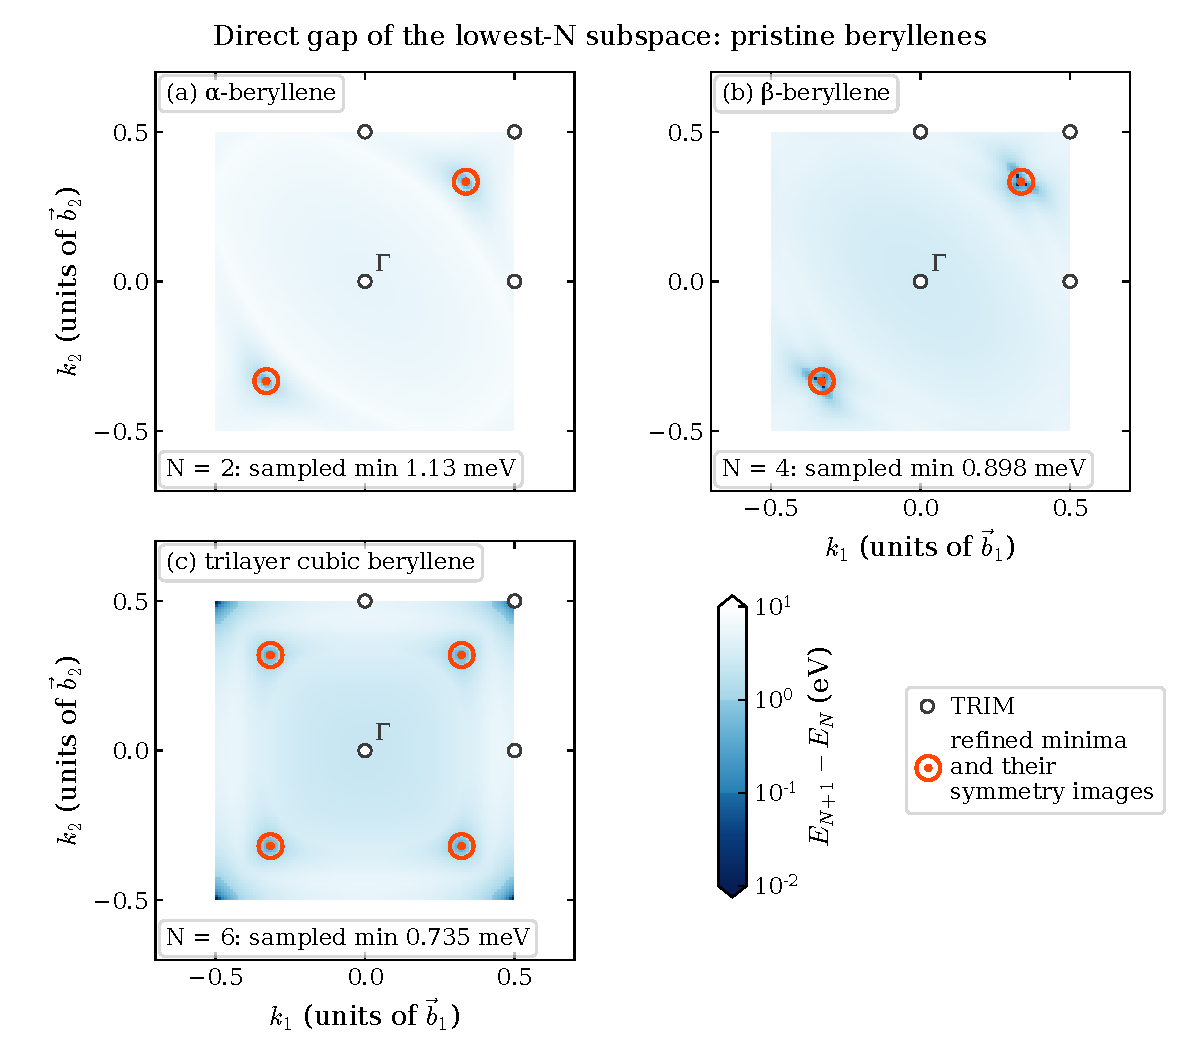
\includegraphics[width=0.80\linewidth]{figures_proj3/topology_direct-gap_pristine_thesis.pdf}
\caption{Direct gap $E_{N+1}-E_{N}$ of the lowest-$N$ subspace over the Brillouin zone for (a) $\alpha$-beryllene,
(b) $\beta$-beryllene,
and (c) trilayer cubic beryllene,
on a logarithmic scale.
The time-reversal invariant momenta,
the refined minima,
and their symmetry images are marked.}
\label{fig:proj3_direct_gap_pristine}
\end{figure}

\begin{figure}[!htbp]
\centering
    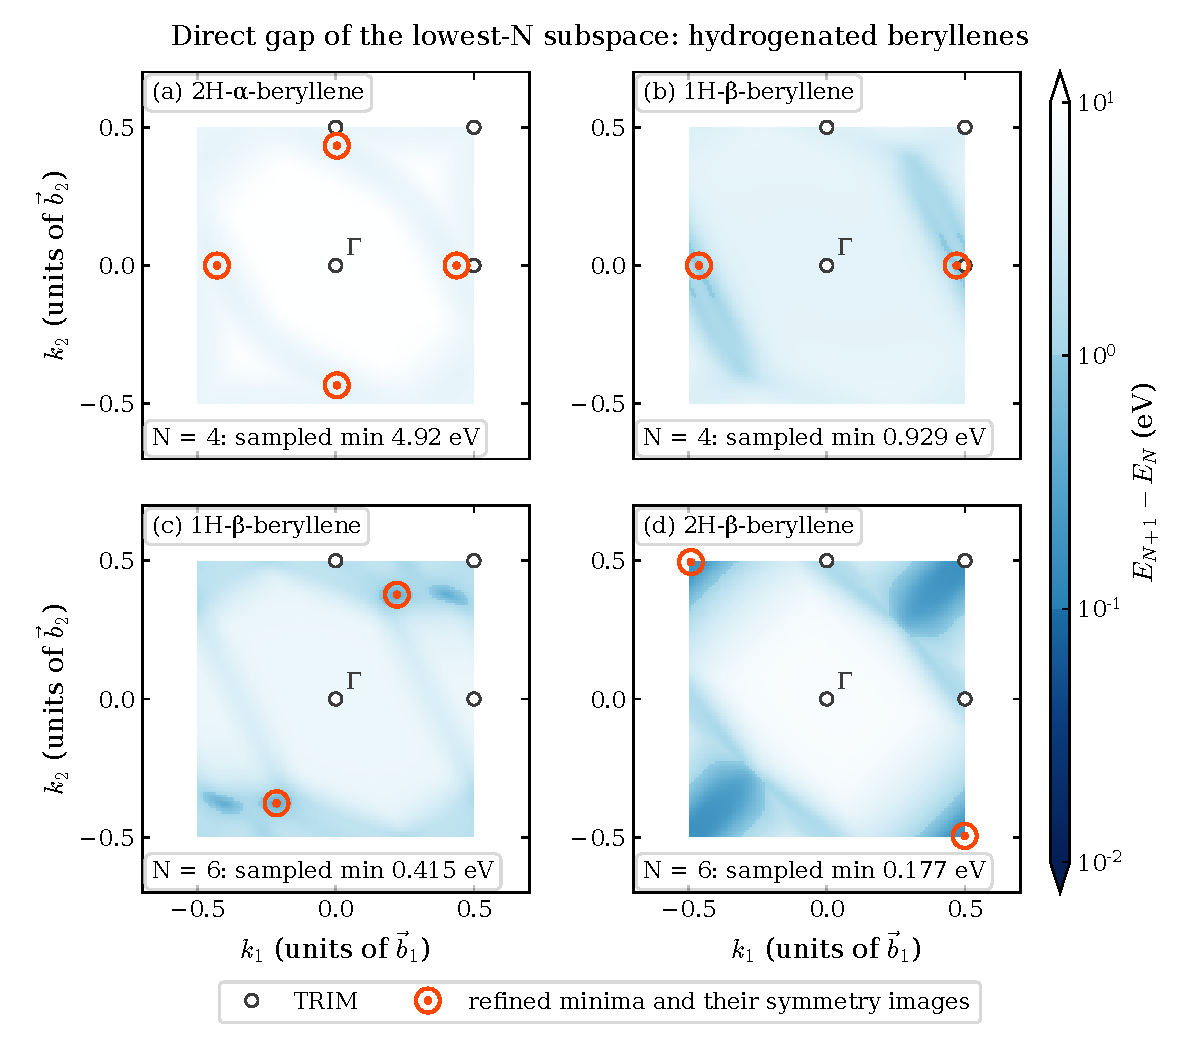
\includegraphics[width=0.80\linewidth]{figures_proj3/topology_direct-gap_hydrogenated_thesis.pdf}
\caption{Direct gap $E_{N+1}-E_{N}$ of the lowest-$N$ subspace over the Brillouin zone for (a) 2H-$\alpha$-beryllene,
(b, c) 1H-$\beta$-beryllene with $N=4$ and $N=6$,
and (d) 2H-$\beta$-beryllene,
shown as in figure~\ref{fig:proj3_direct_gap_pristine}.}
\label{fig:proj3_direct_gap_hydrogenated}
\end{figure}

\begin{figure}[!htbp]
\centering
    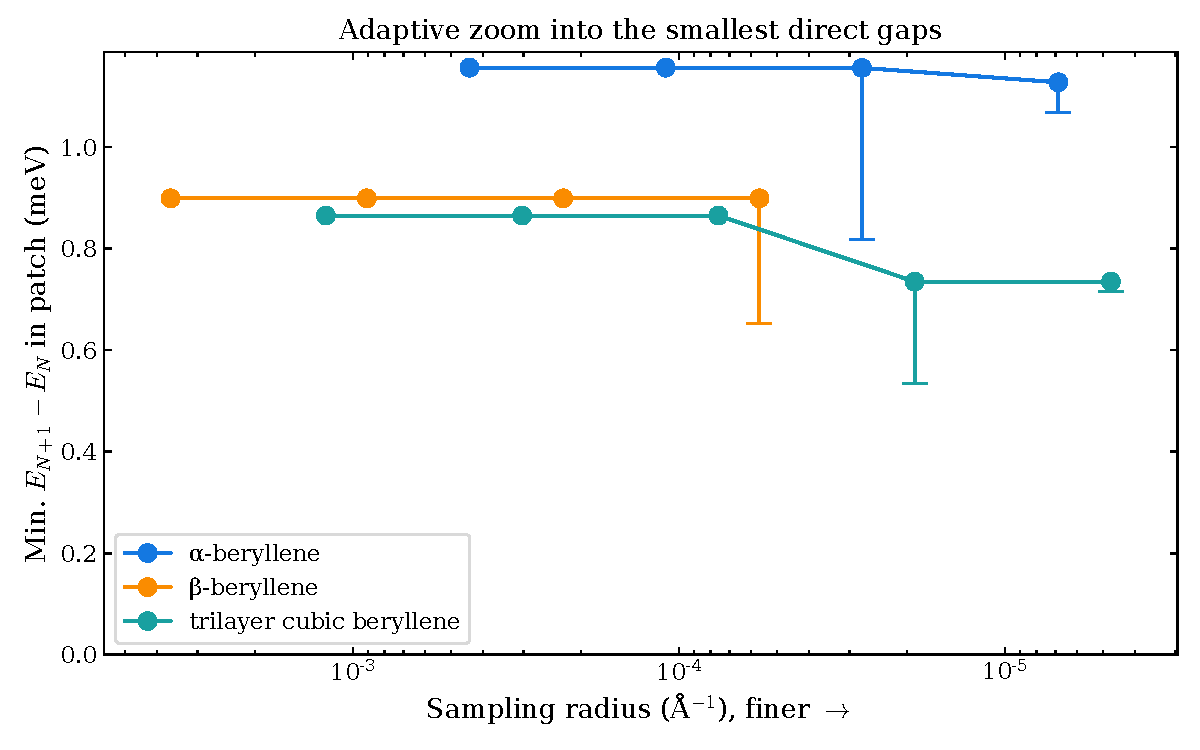
\includegraphics[width=0.80\linewidth]{figures_proj3/topology_gap-zoom_thesis.pdf}
\caption{Minimum direct gap in each refinement patch as a function of the sampling radius for $\alpha$-beryllene,
$\beta$-beryllene,
and trilayer cubic beryllene.
The lower ends of the vertical bars show the lower bounds estimated from the local slope of the gap.}
\label{fig:proj3_gap_zoom}
\end{figure}

\begin{figure}[!htbp]
\centering
    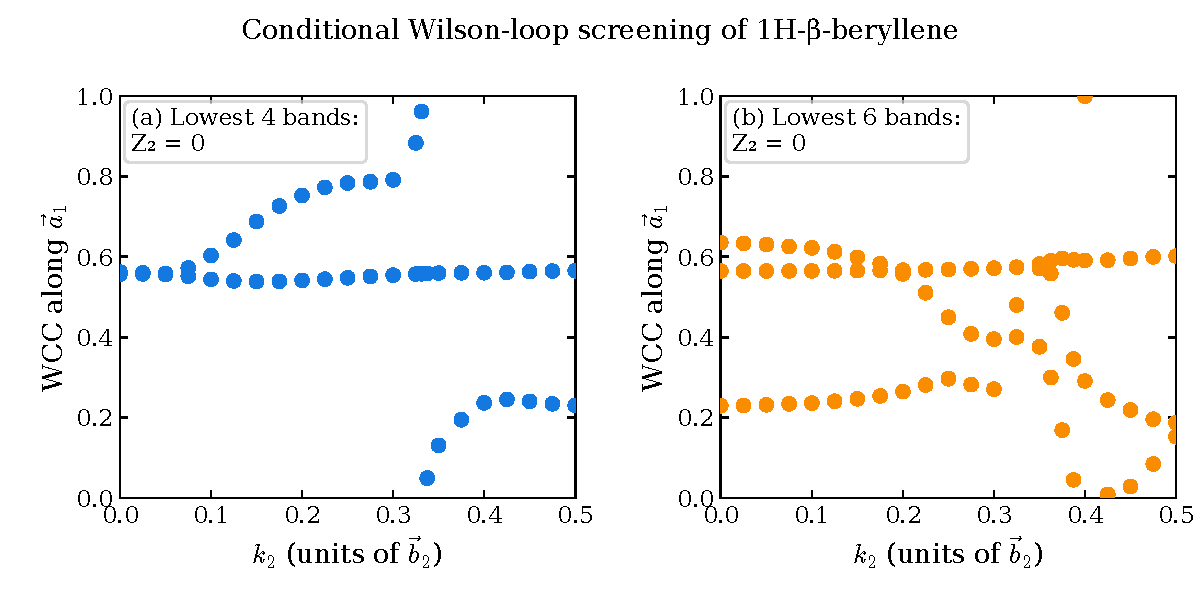
\includegraphics[width=0.80\linewidth]{figures_proj3/topology_wcc_1H-beta-beryllene_thesis.pdf}
\caption{Wannier charge centres of 1H-$\beta$-beryllene along $\vec{a}_{1}$ as functions of $k_{2}$ over half of the Brillouin zone,
for (a) the lowest four bands and (b) the lowest six bands.}
\label{fig:proj3_wcc}
\end{figure}

\subsection*{Additional optical spectra}

Additional optical spectra are shown in figures~\ref{fig:proj3_reflectivity_alpha_beta}--\ref{fig:proj3_optical_hydrogenated_extinction}.
Figures~\ref{fig:proj3_reflectivity_alpha_beta} and~\ref{fig:proj3_energy_loss_alpha_beta} show the reflectivity and energy-loss spectrum for $\alpha$-beryllene and $\beta$-beryllene.
Figures~\ref{fig:proj3_optical_clean}--\ref{fig:proj3_optical_clean_extinction} compare the pristine bulk and two-dimensional beryllium structures,
whereas figures~\ref{fig:proj3_optical_hydrogenated}--\ref{fig:proj3_optical_hydrogenated_extinction} compare the corresponding hydrogen-functionalized structures.
These spectra are scalar comparisons derived from the individual Cartesian diagonal components of the dielectric tensor,
following the definitions in section~\ref{3_methods}.
For 1H-$\beta$-beryllene and 2H-$\beta$-beryllene,
off-diagonal dielectric coupling is not included in these scalar quantities.

\begin{figure}[!htbp]
\centering
    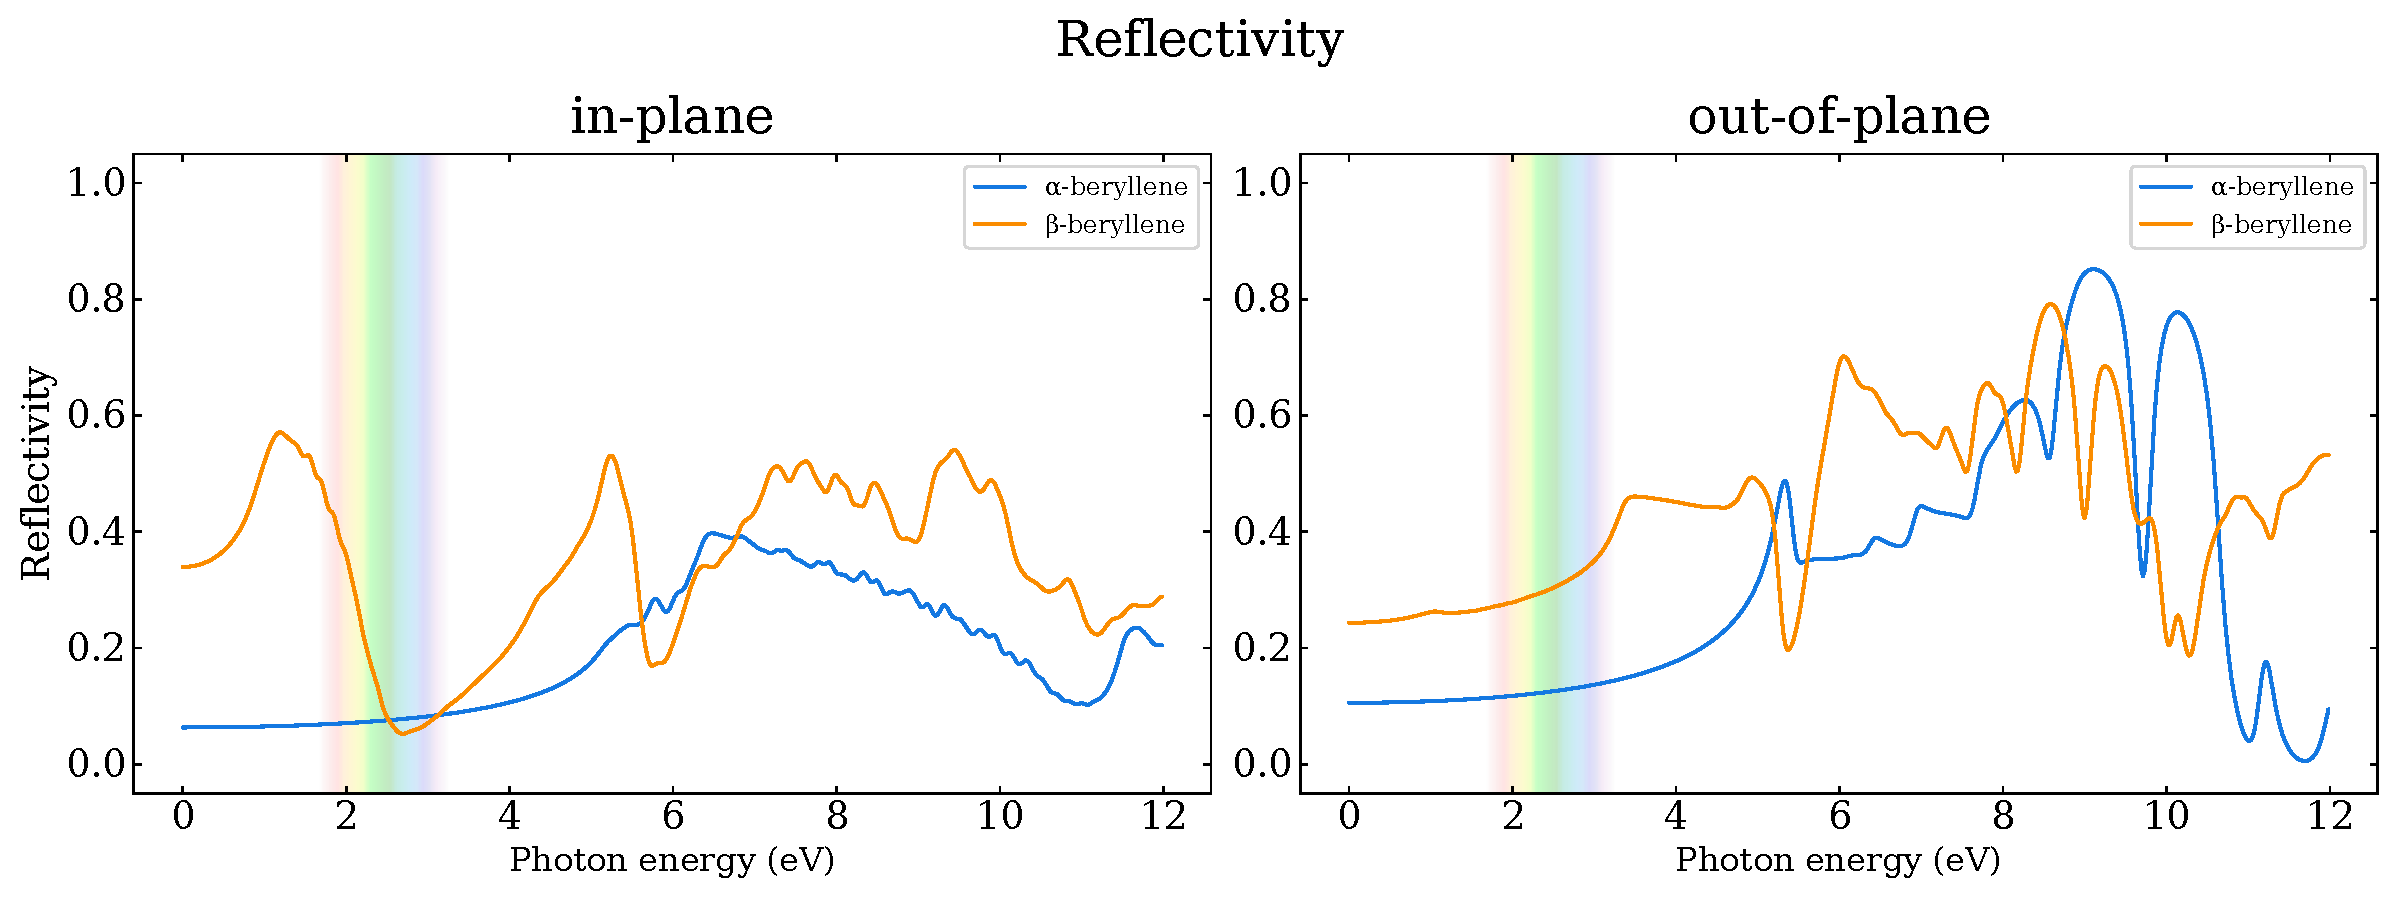
\includegraphics[width=0.80\linewidth]{figures_proj3/optics_alpha-beta_reflectivity_thesis.pdf}
\caption{Reflectivity for the in-plane and out-of-plane directions as a function of photon energy for $\alpha$-beryllene and $\beta$-beryllene.
The in-plane and out-of-plane curves correspond to the $xx$ and $zz$ components, respectively.}
\label{fig:proj3_reflectivity_alpha_beta}
\end{figure}

\begin{figure}[!htbp]
\centering
    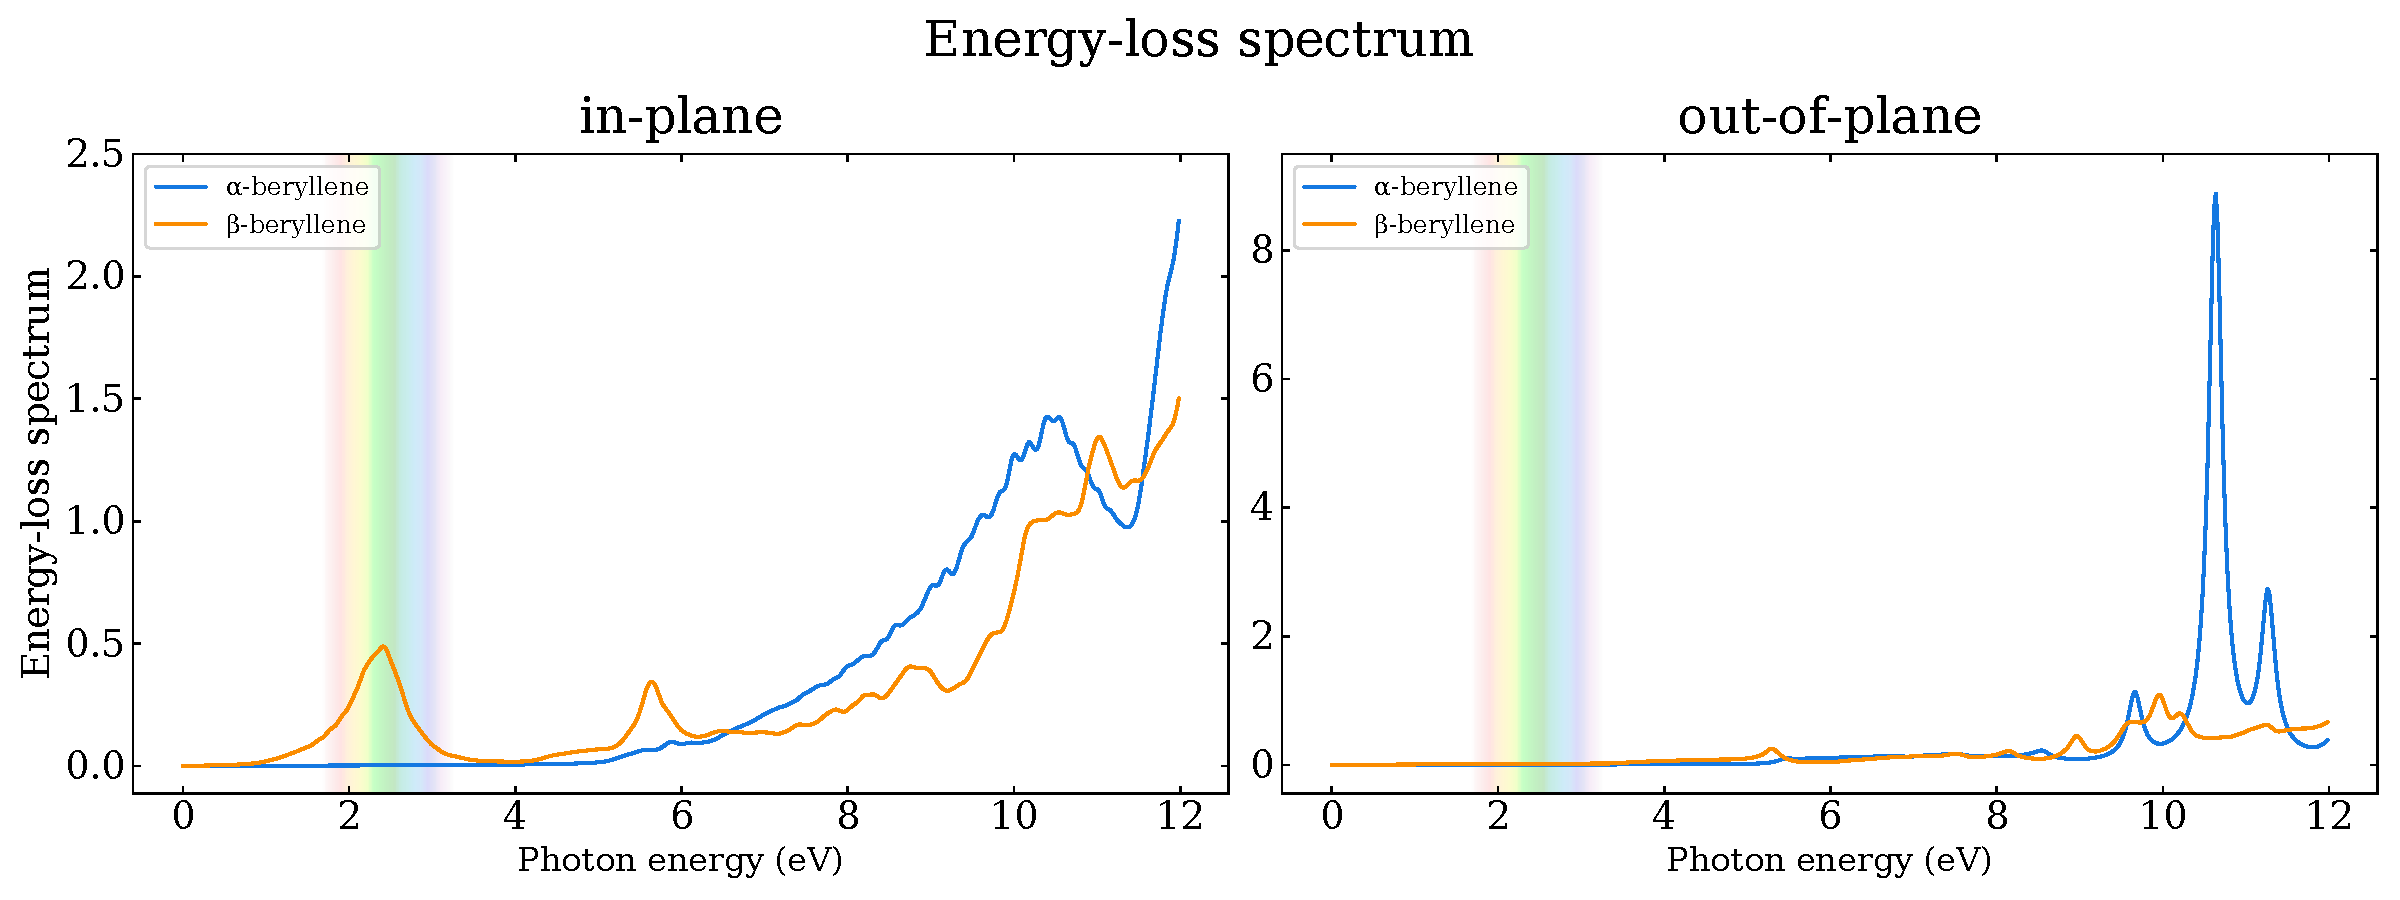
\includegraphics[width=0.80\linewidth]{figures_proj3/optics_alpha-beta_energy-loss_thesis.pdf}
\caption{Energy-loss spectrum for the in-plane and out-of-plane directions as a function of photon energy for $\alpha$-beryllene and $\beta$-beryllene.
The in-plane and out-of-plane curves correspond to the $xx$ and $zz$ components, respectively.}
\label{fig:proj3_energy_loss_alpha_beta}
\end{figure}

\begin{figure}[!htbp]
\centering
    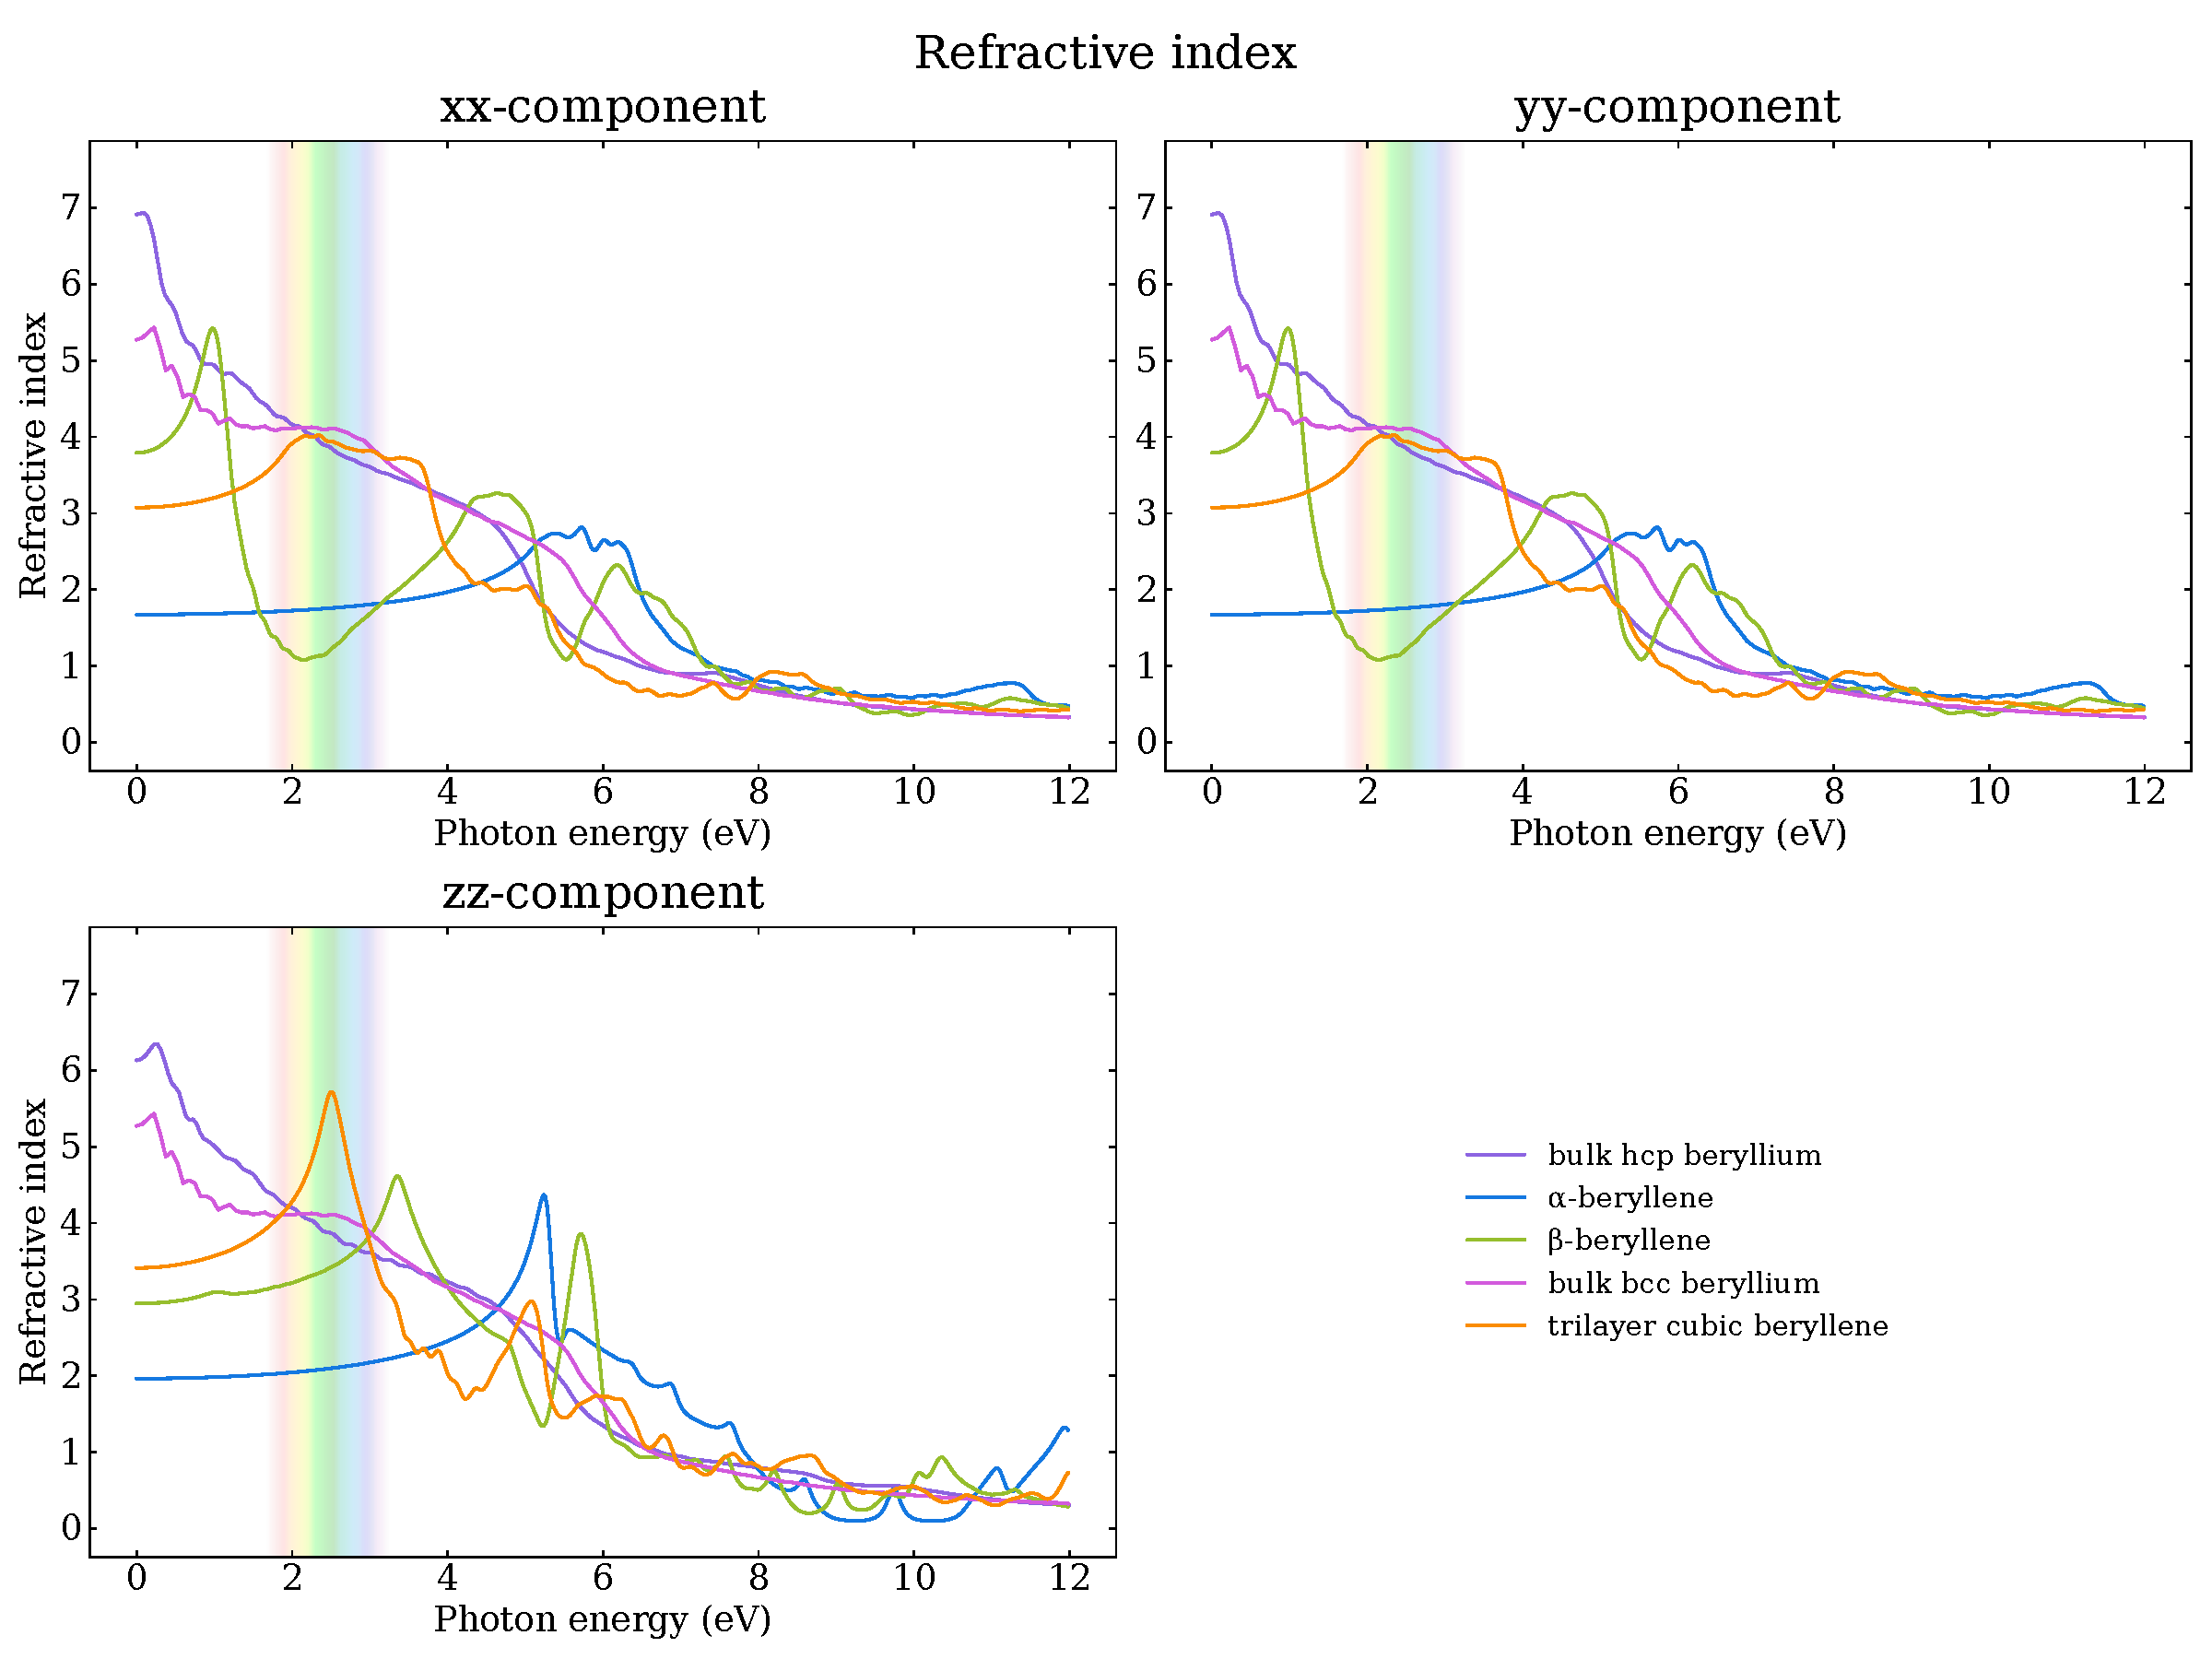
\includegraphics[width=0.80\linewidth]{figures_proj3/optics_pristine_refractive_thesis.pdf}
\caption{Refractive index for bulk hcp beryllium, $\alpha$-beryllene, $\beta$-beryllene,
bulk bcc beryllium, and trilayer cubic beryllene.
The spectra are shown for the $xx$,
$yy$,
and $zz$ components as functions of photon energy.}
\label{fig:proj3_optical_clean}
\end{figure}

\begin{figure}[!htbp]
\centering
    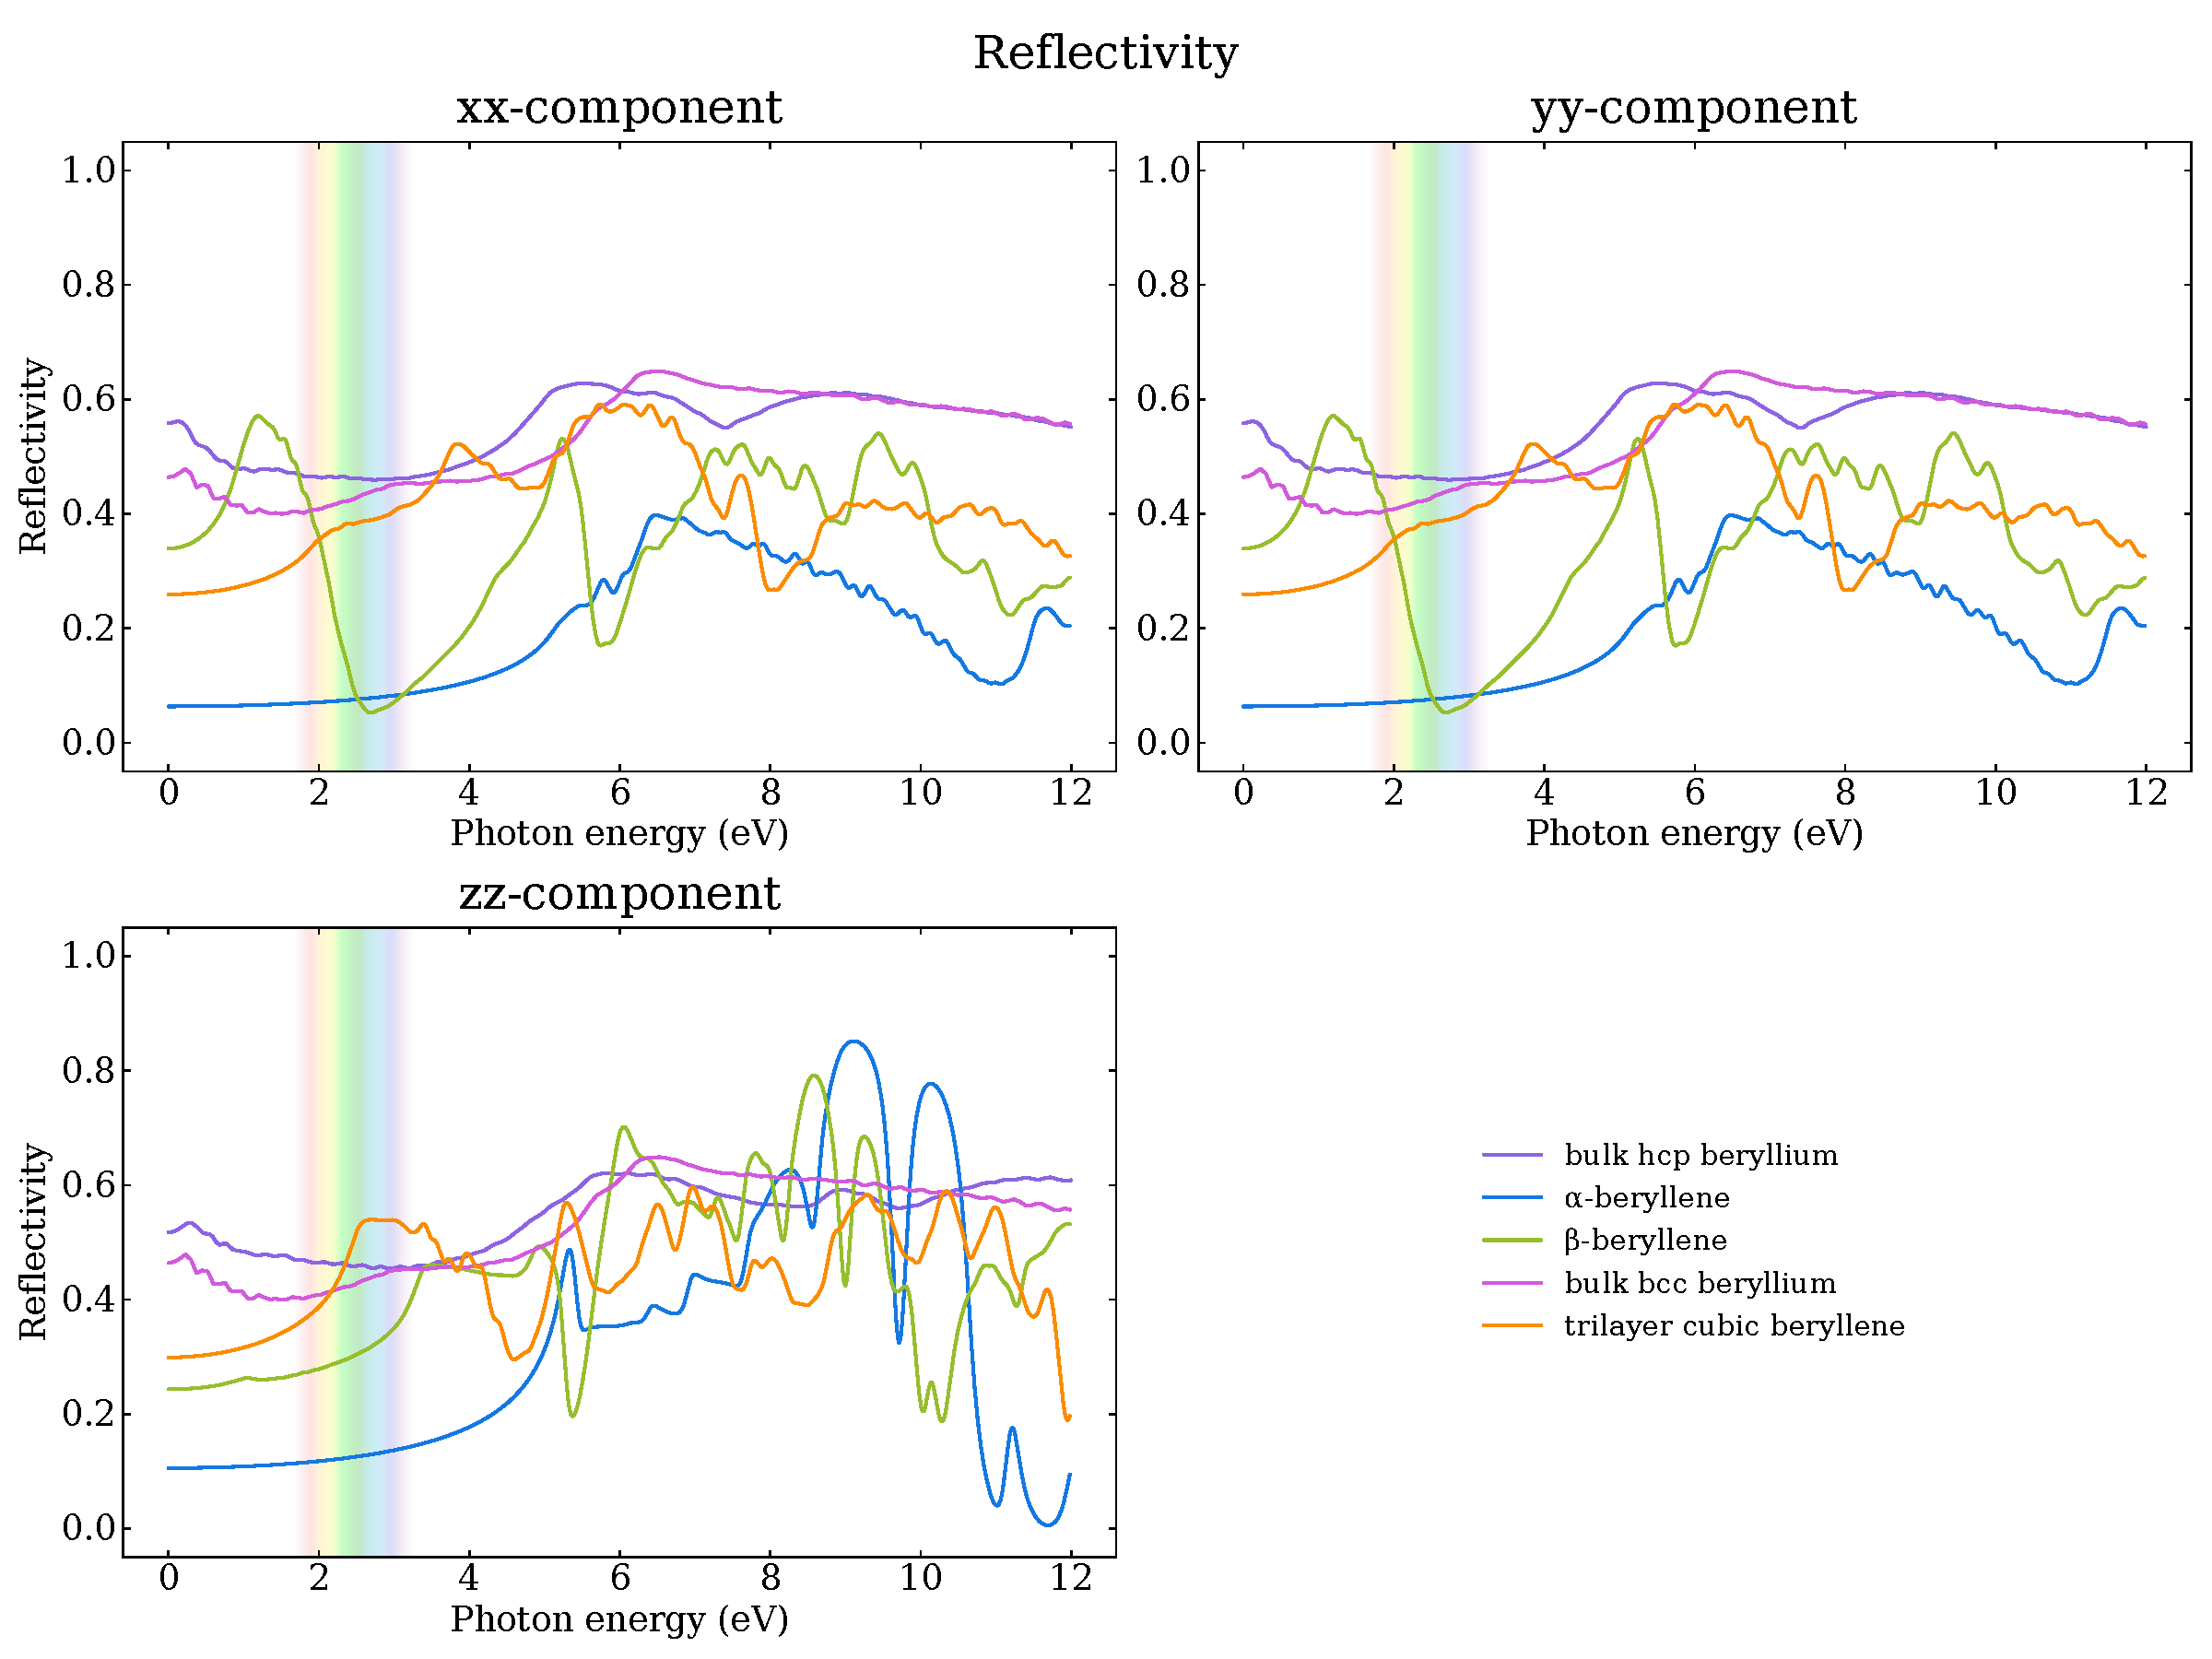
\includegraphics[width=0.80\linewidth]{figures_proj3/optics_pristine_reflectivity_thesis.pdf}
\caption{Reflectivity for bulk hcp beryllium, $\alpha$-beryllene, $\beta$-beryllene,
bulk bcc beryllium, and trilayer cubic beryllene.
The spectra are shown for the $xx$,
$yy$,
and $zz$ components as functions of photon energy.}
\label{fig:proj3_optical_clean_reflectivity}
\end{figure}

\begin{figure}[!htbp]
\centering
    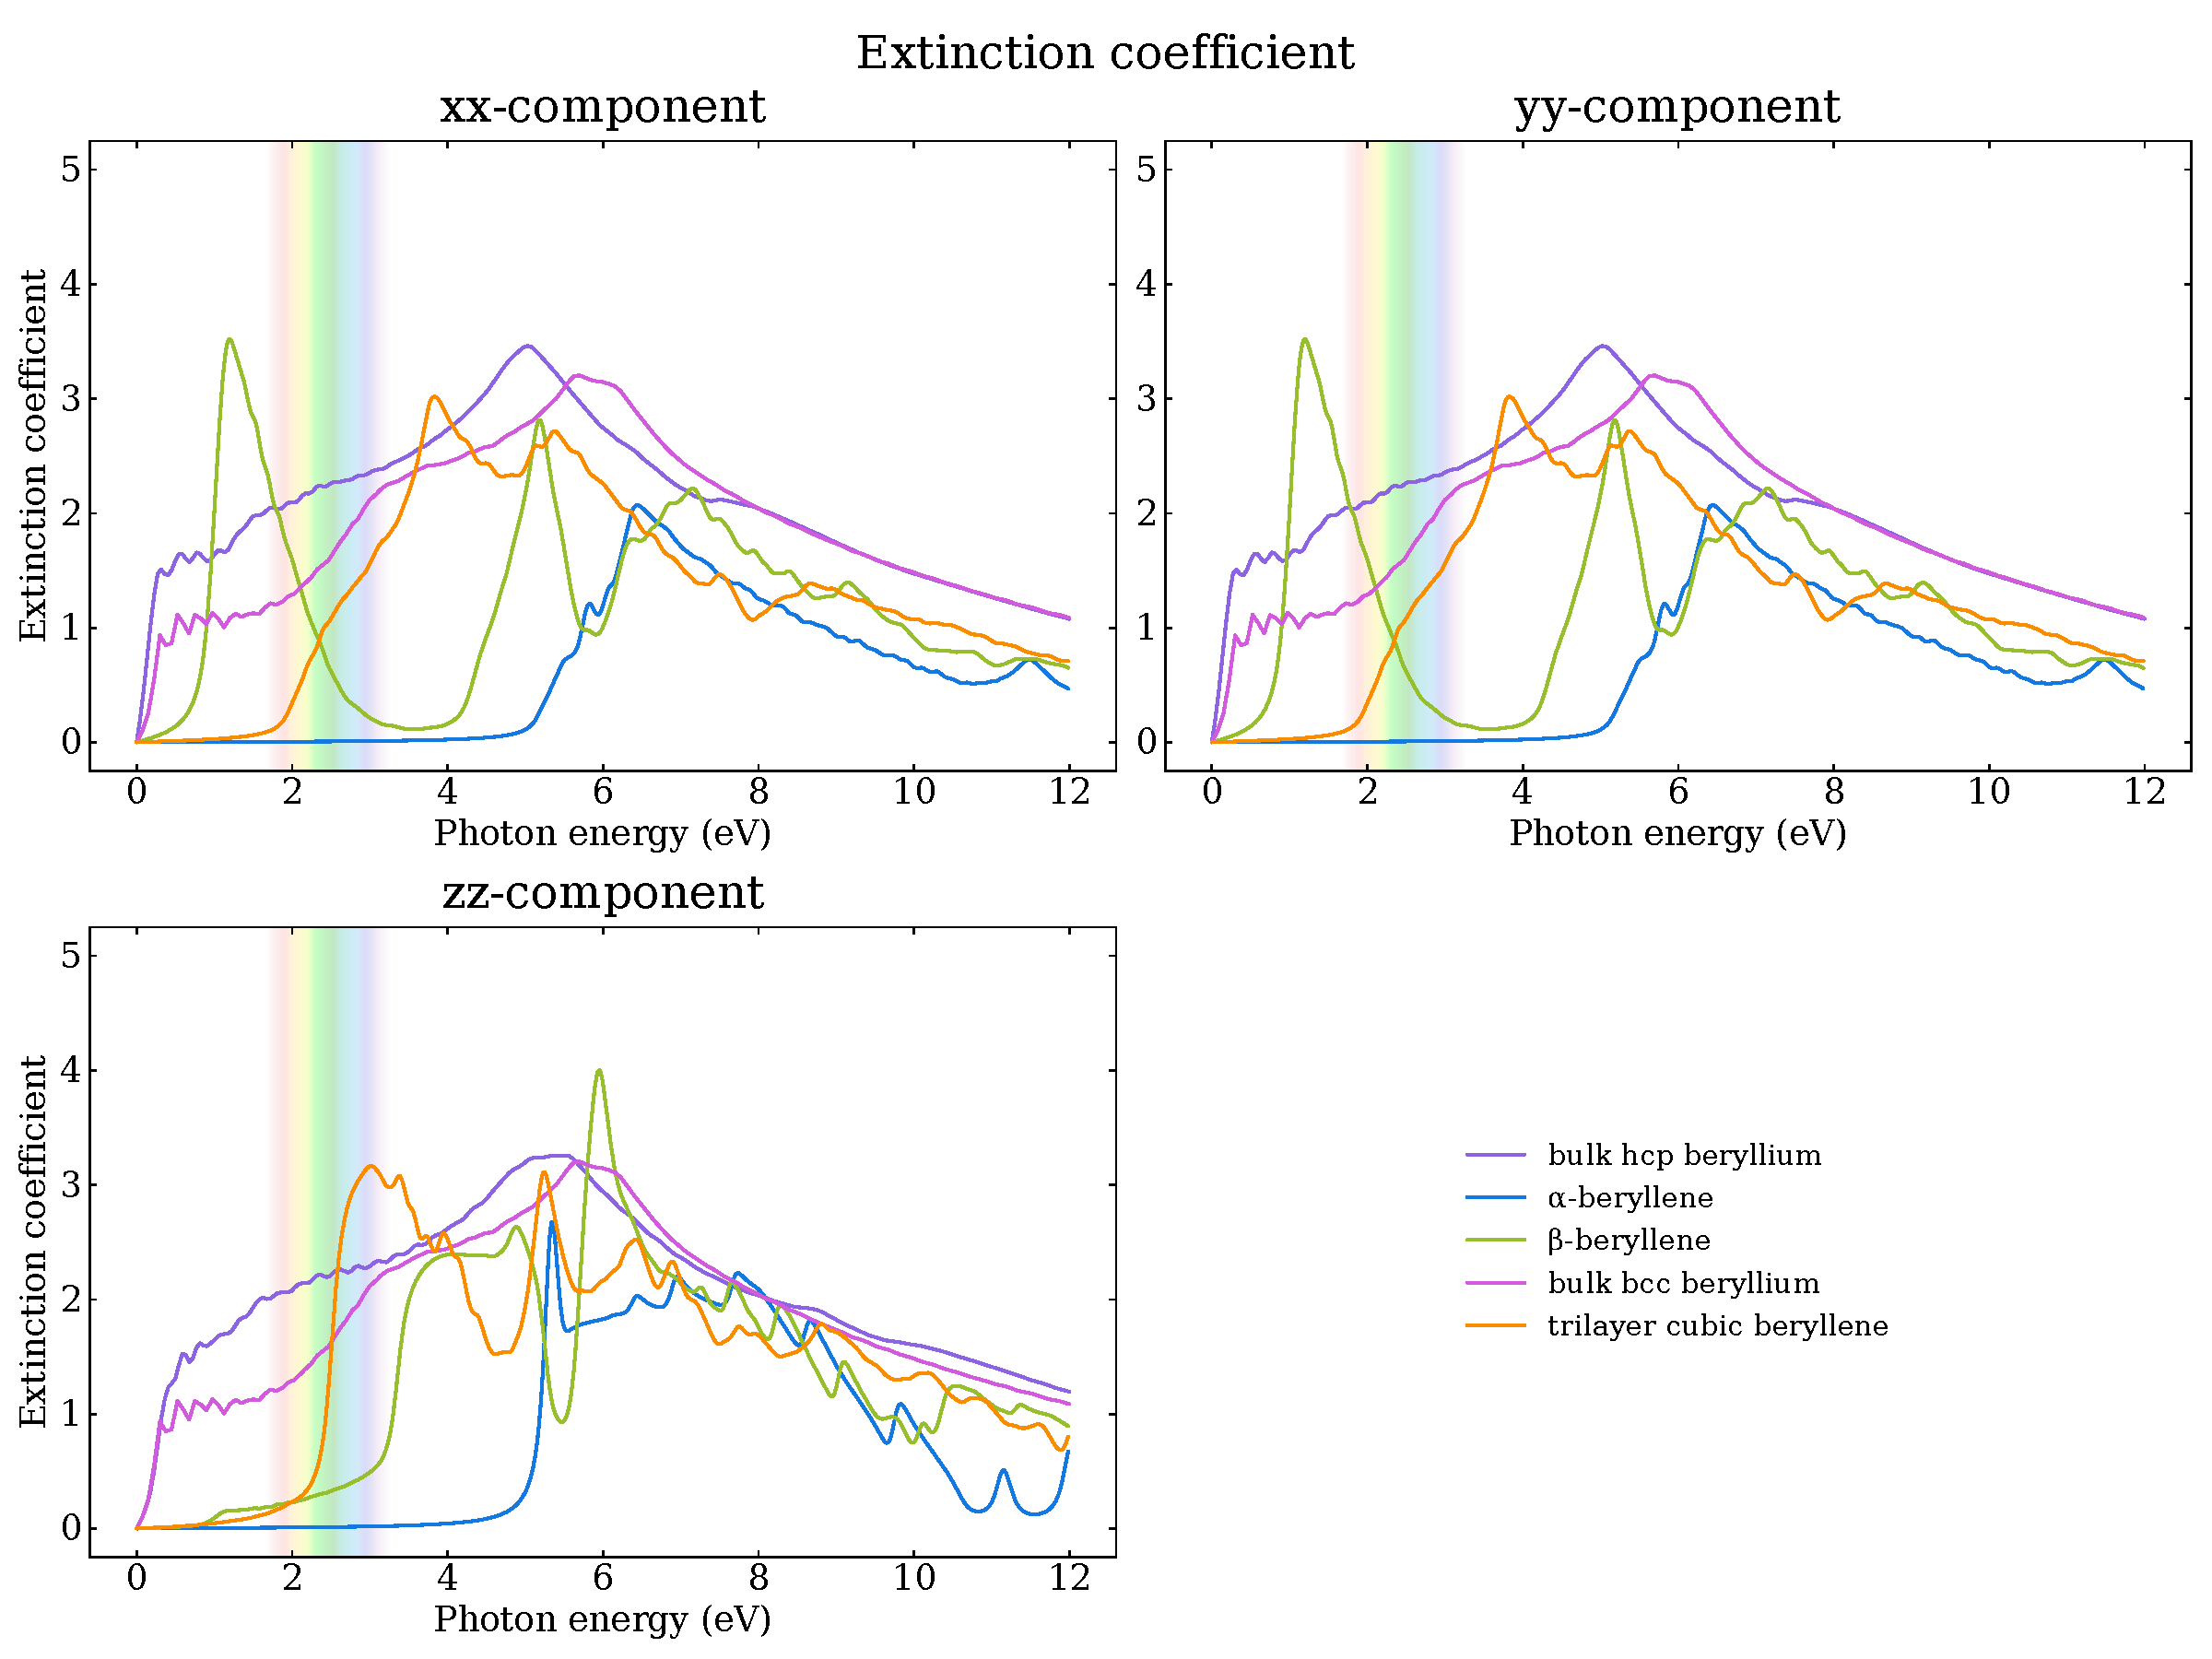
\includegraphics[width=0.80\linewidth]{figures_proj3/optics_pristine_extinction_thesis.pdf}
\caption{Extinction coefficient for bulk hcp beryllium, $\alpha$-beryllene, $\beta$-beryllene,
bulk bcc beryllium, and trilayer cubic beryllene.
The spectra are shown for the $xx$,
$yy$,
and $zz$ components as functions of photon energy.}
\label{fig:proj3_optical_clean_extinction}
\end{figure}

\begin{figure}[!htbp]
\centering
    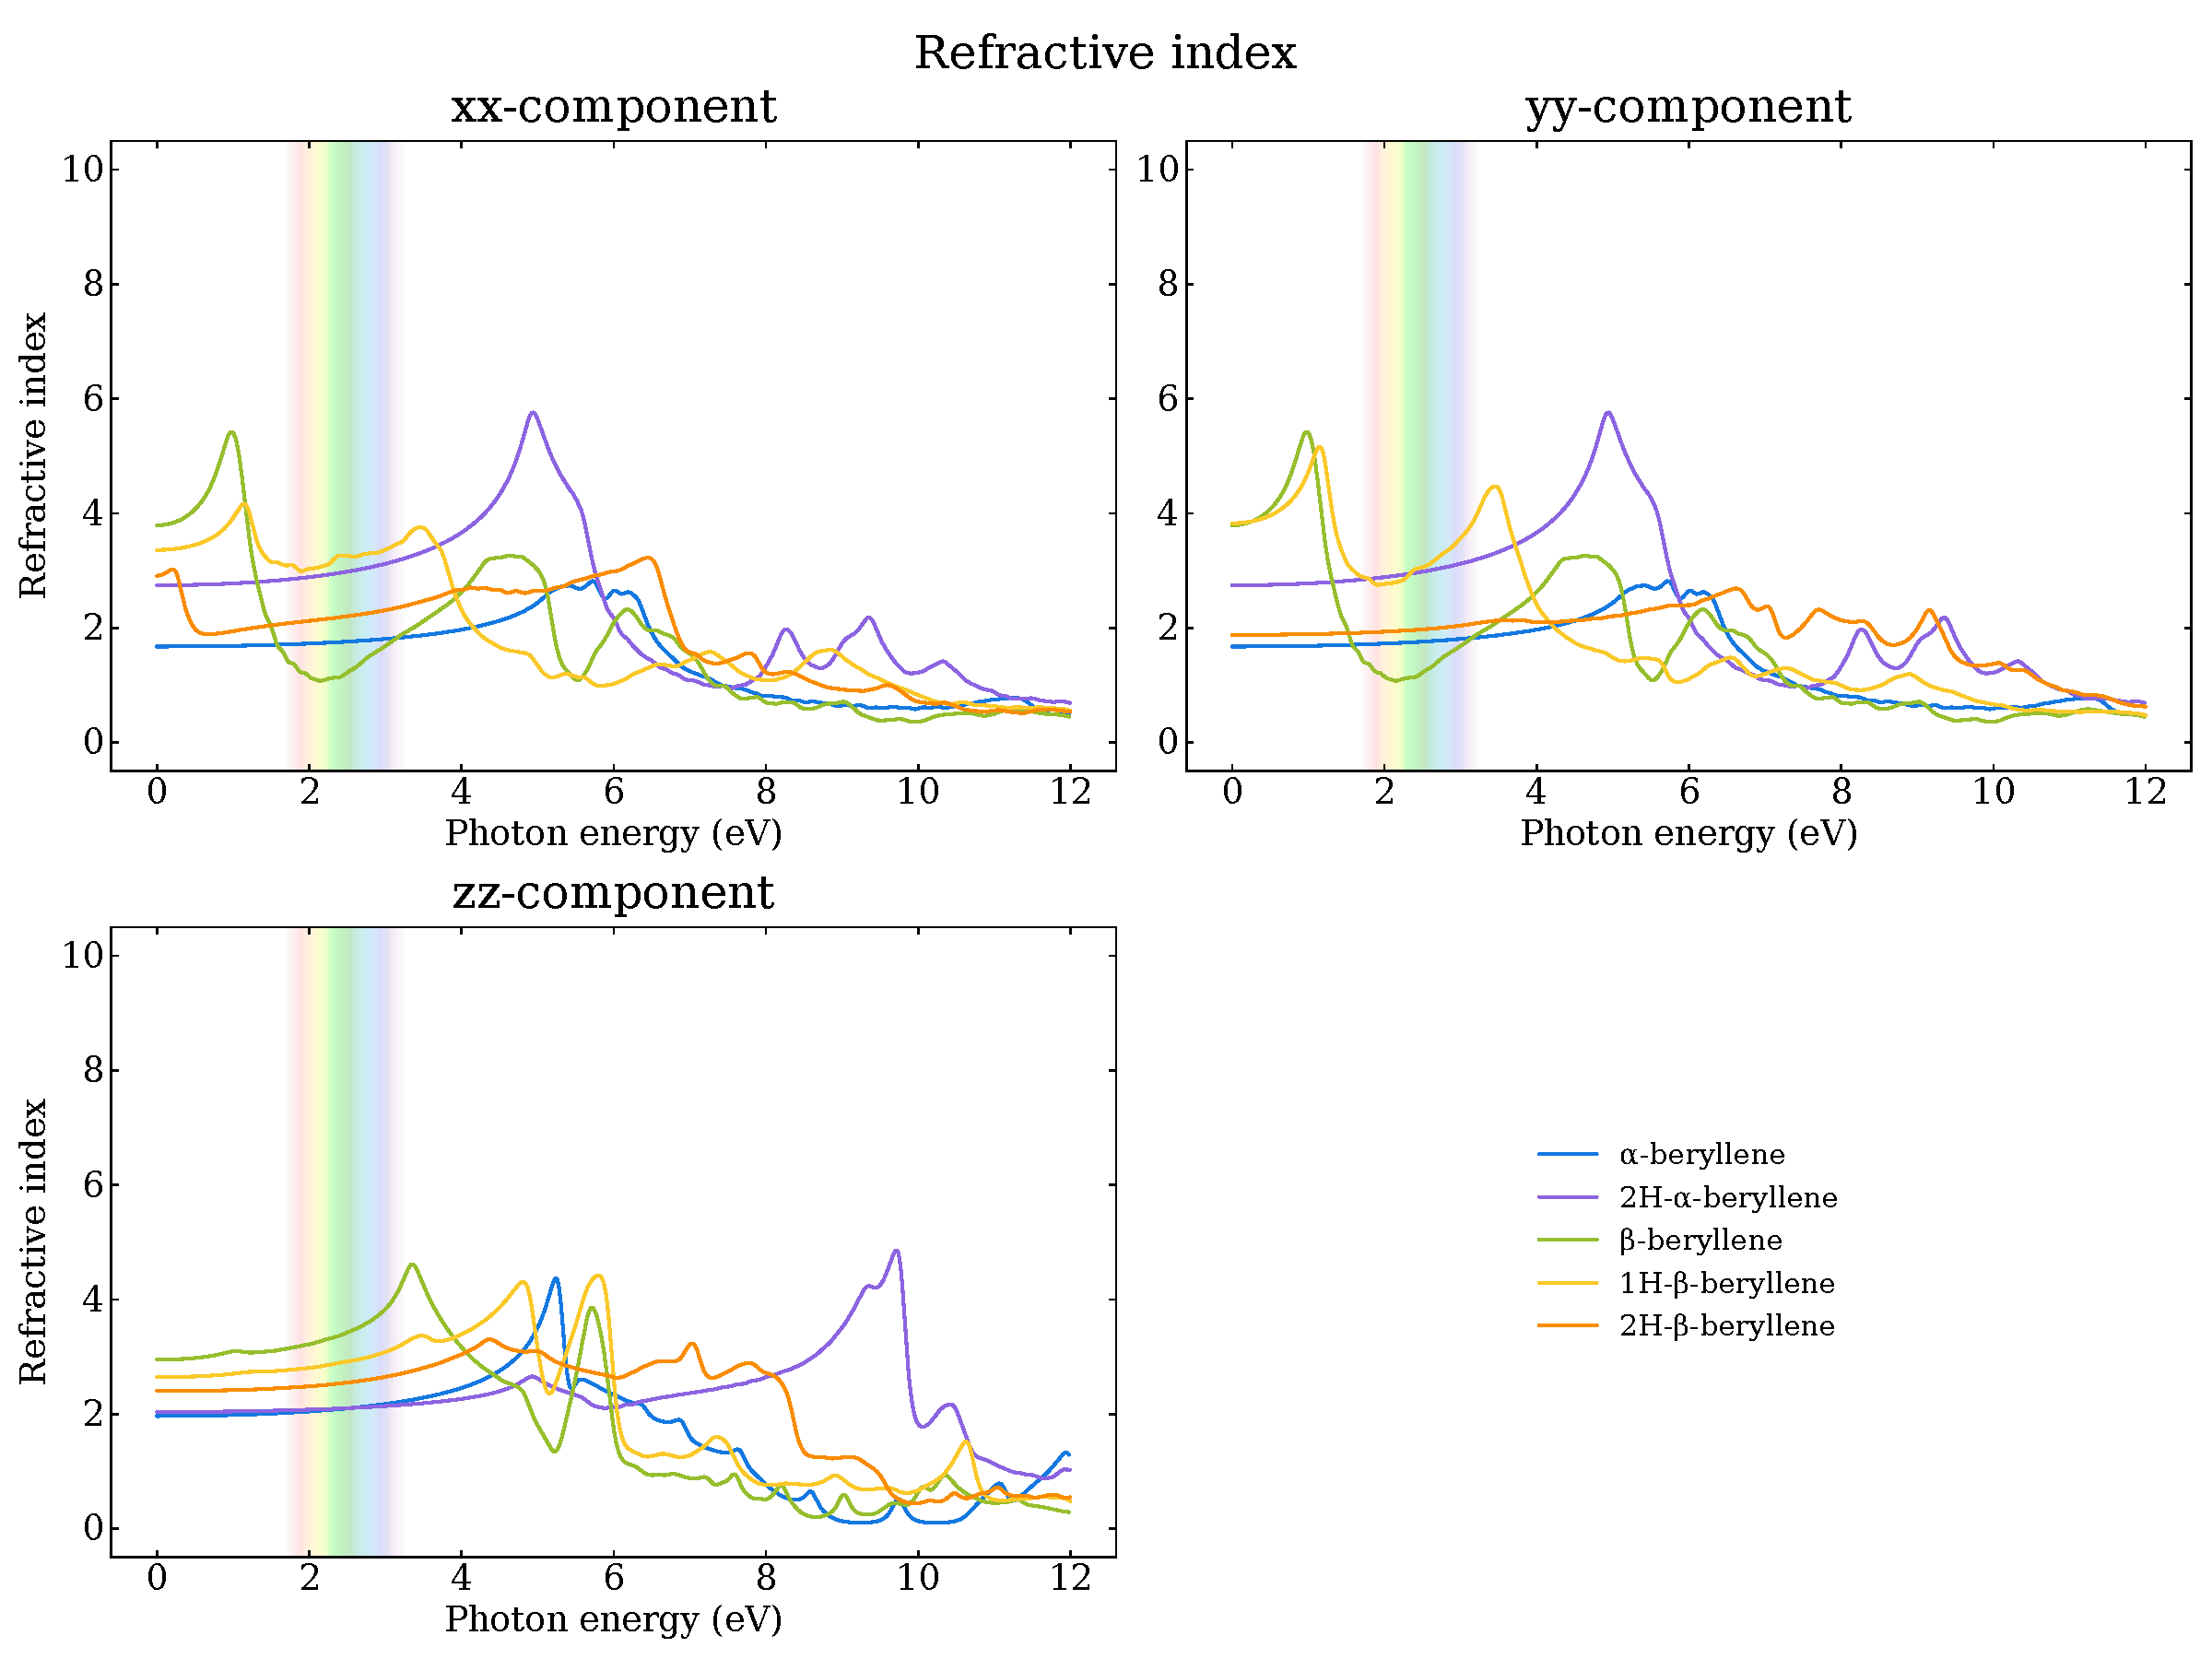
\includegraphics[width=0.80\linewidth]{figures_proj3/optics_hydrogenated_refractive_thesis.pdf}
\caption{Refractive index for pristine and hydrogen-functionalized $\alpha$-beryllene and $\beta$-beryllene structures.
The spectra are shown for the $xx$,
$yy$,
and $zz$ components as functions of photon energy.}
\label{fig:proj3_optical_hydrogenated}
\end{figure}

\begin{figure}[!htbp]
\centering
    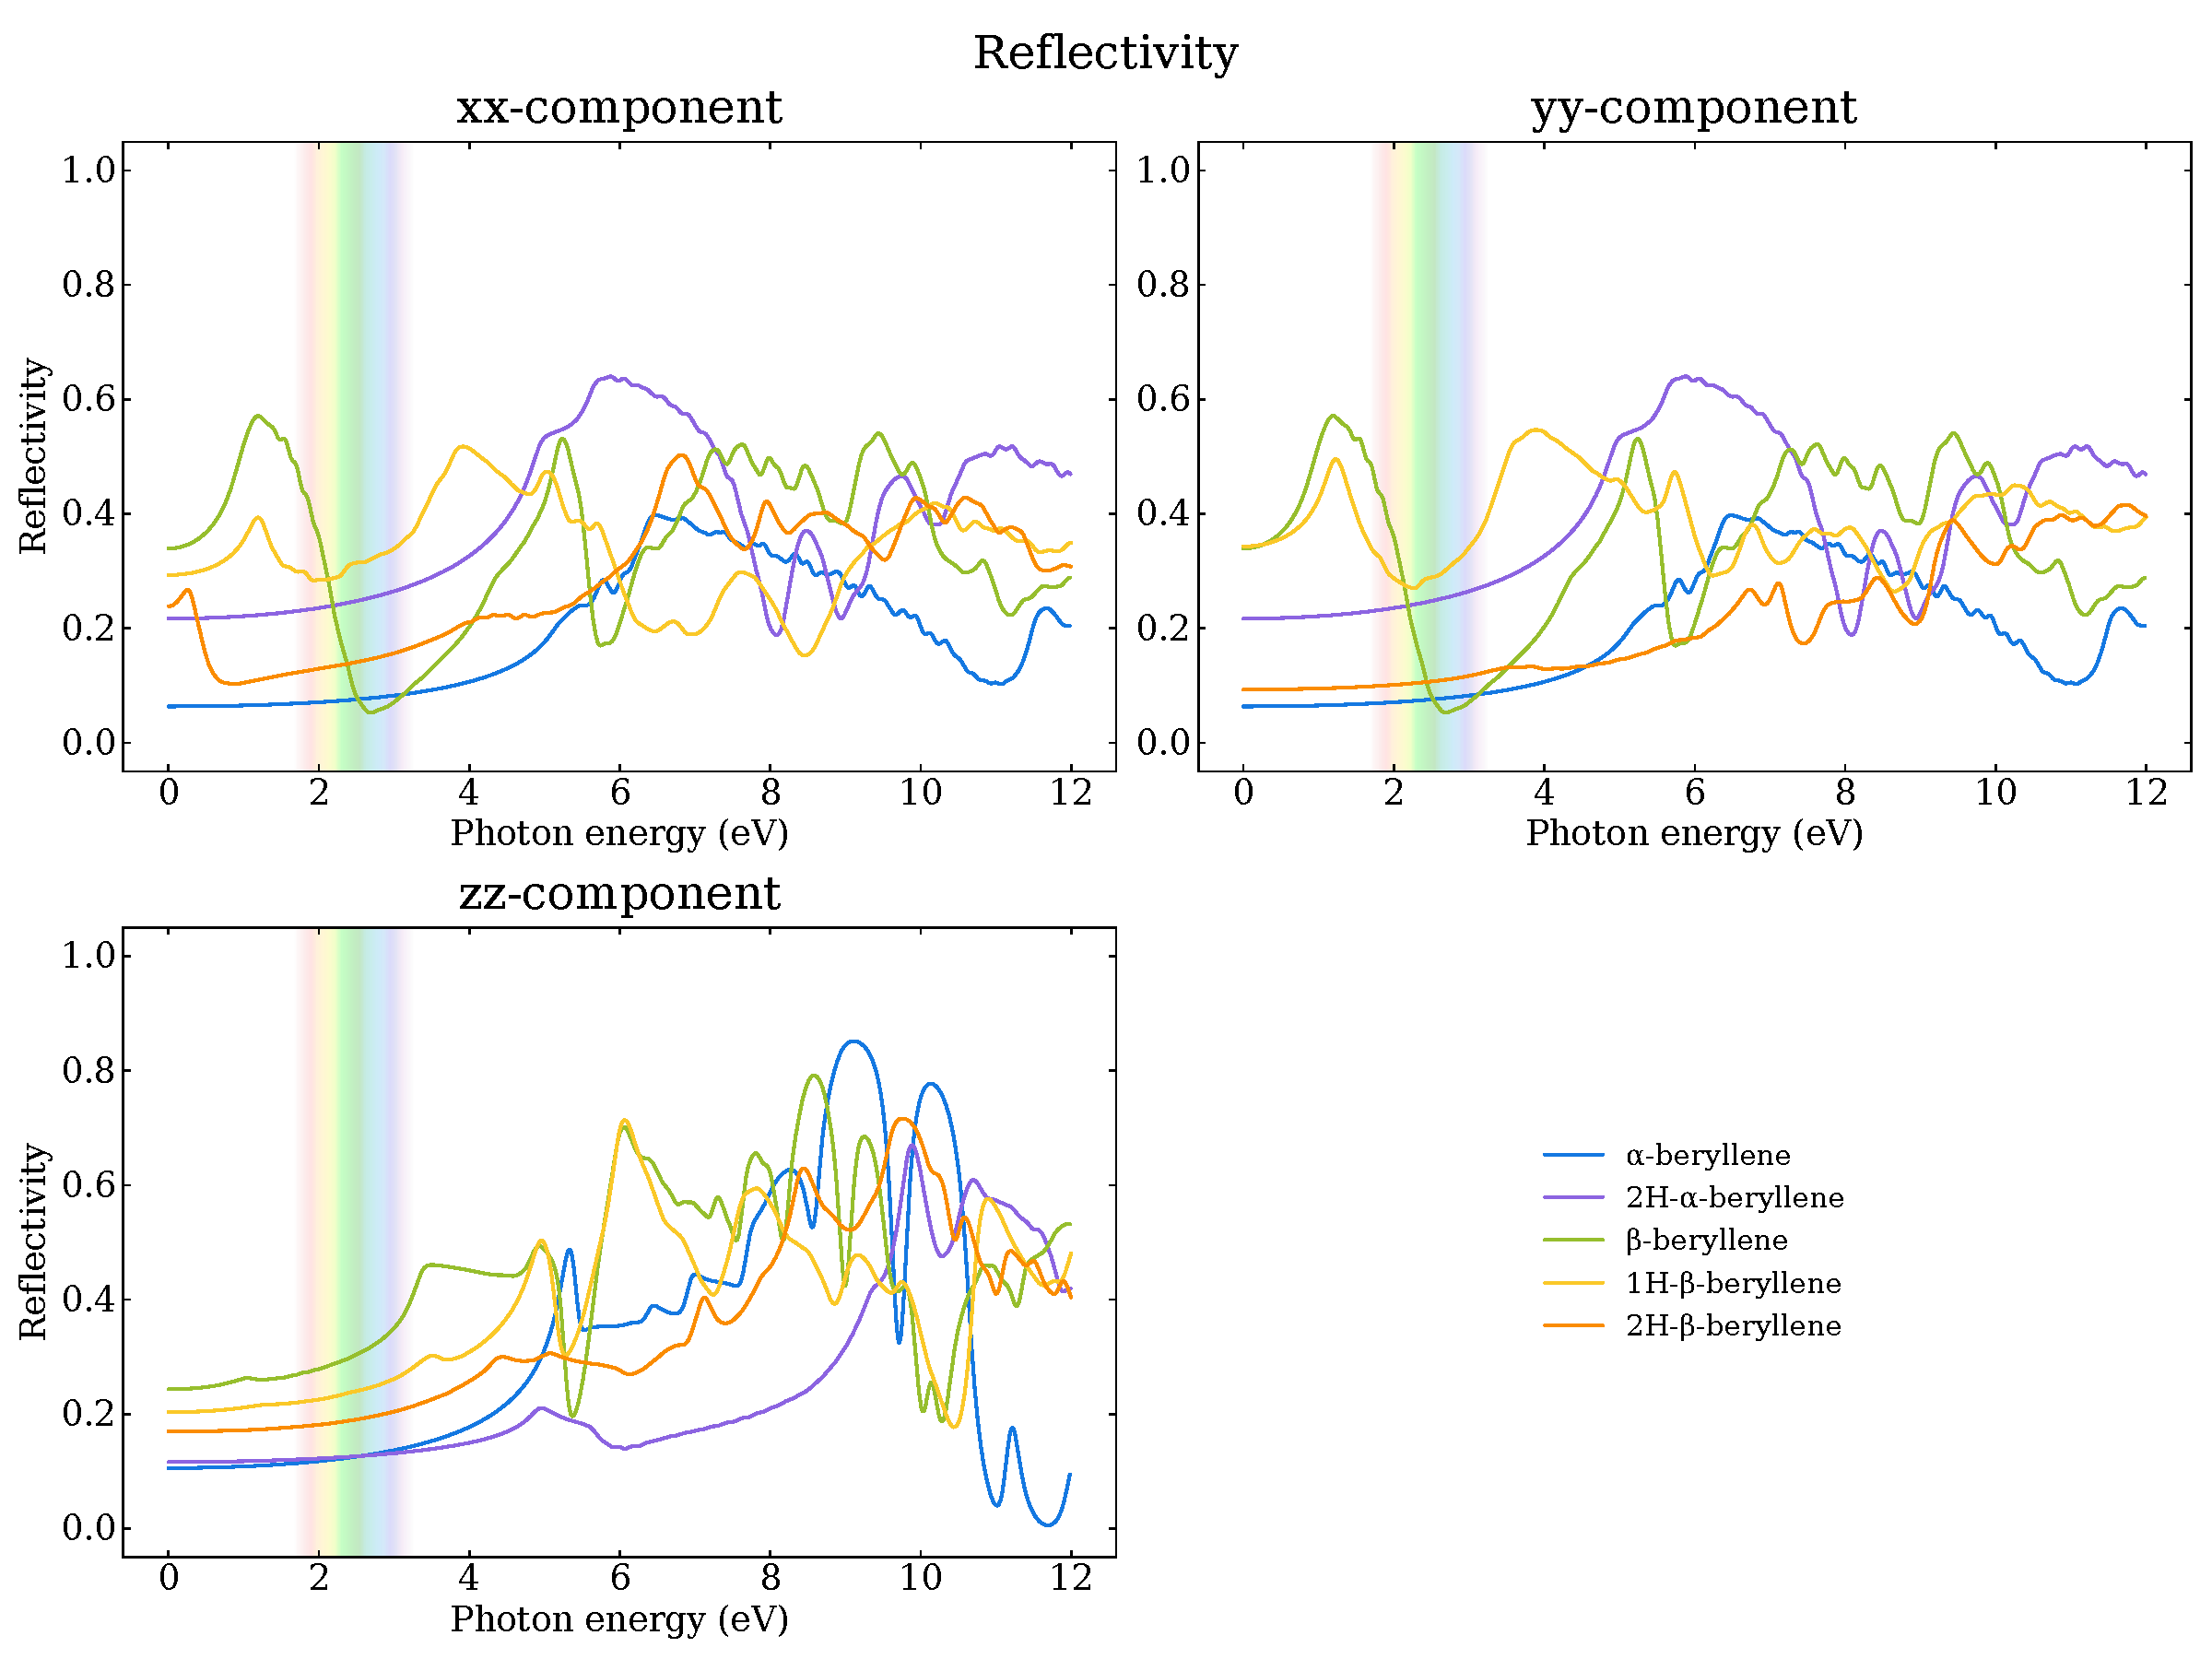
\includegraphics[width=0.80\linewidth]{figures_proj3/optics_hydrogenated_reflectivity_thesis.pdf}
\caption{Reflectivity for pristine and hydrogen-functionalized $\alpha$-beryllene and $\beta$-beryllene structures.
The spectra are shown for the $xx$,
$yy$,
and $zz$ components as functions of photon energy.}
\label{fig:proj3_optical_hydrogenated_reflectivity}
\end{figure}

\begin{figure}[!htbp]
\centering
    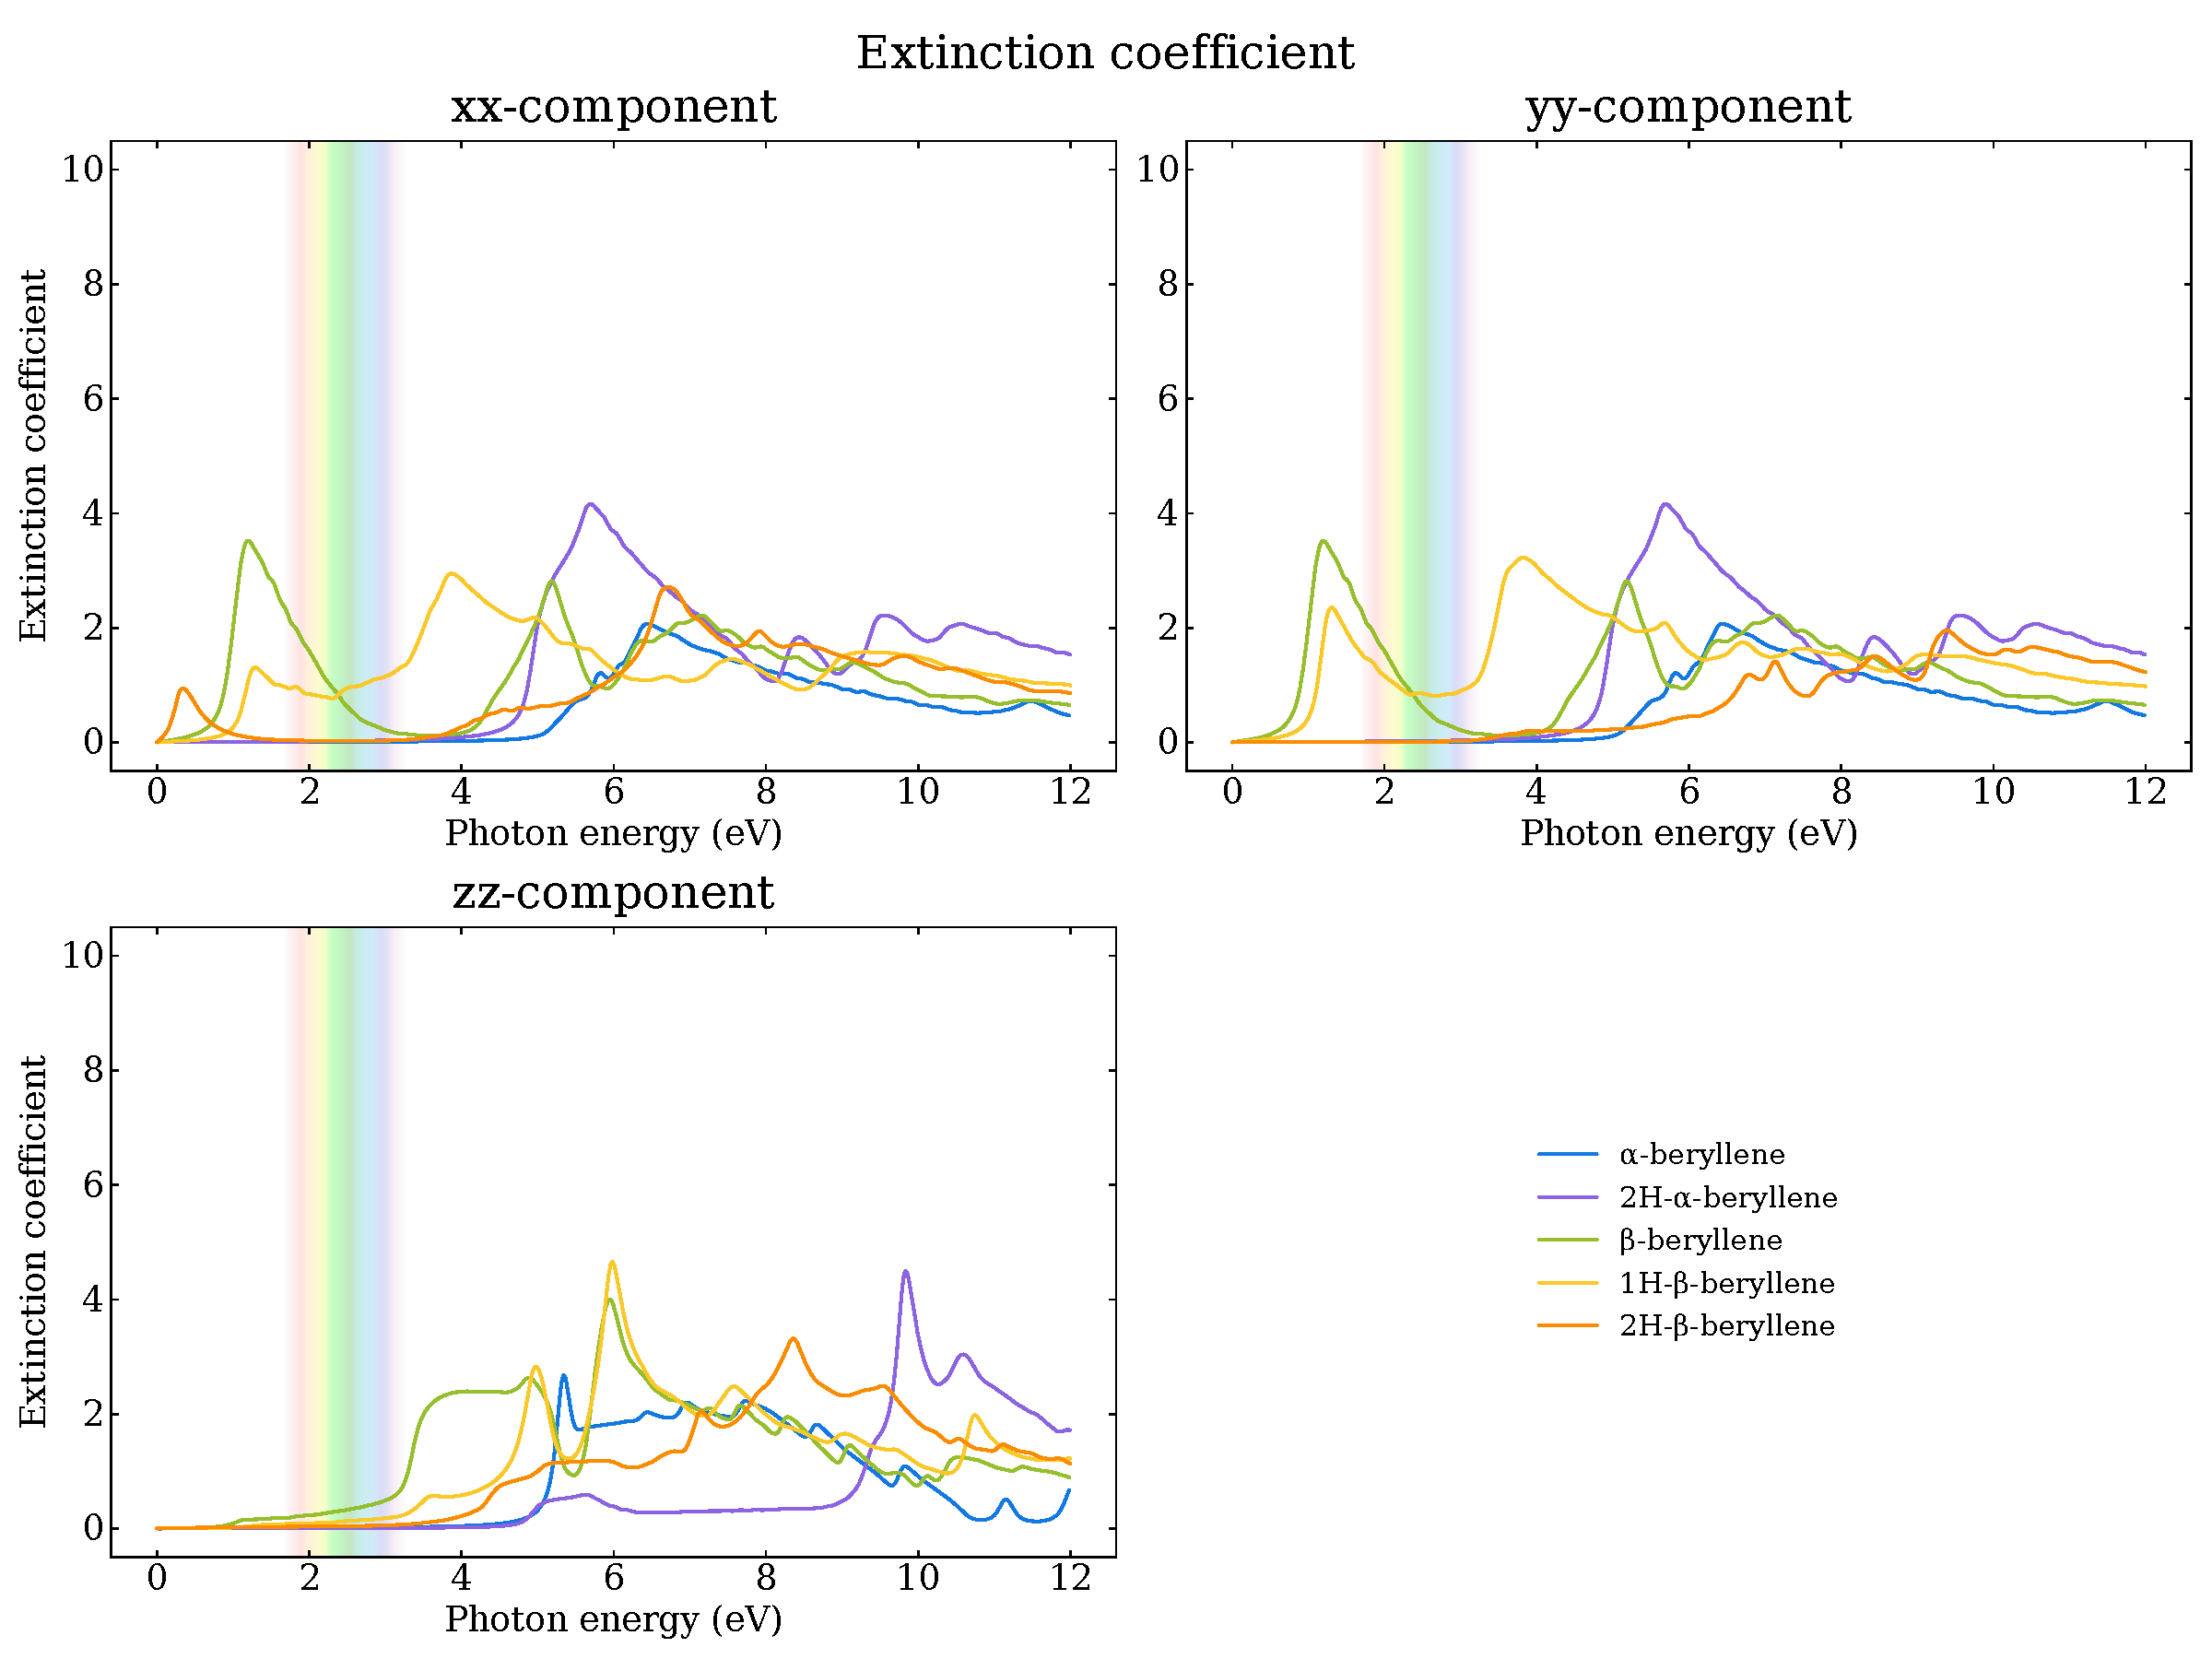
\includegraphics[width=0.80\linewidth]{figures_proj3/optics_hydrogenated_extinction_thesis.pdf}
\caption{Extinction coefficient for pristine and hydrogen-functionalized $\alpha$-beryllene and $\beta$-beryllene structures.
The spectra are shown for the $xx$,
$yy$,
and $zz$ components as functions of photon energy.}
\label{fig:proj3_optical_hydrogenated_extinction}
\end{figure}
